%!TEX program = xelatex
\documentclass[11pt, a4paper]{report}
\usepackage[legalpaper, a4paper, margin=2.5cm]{geometry}
\usepackage{csquotes}
\usepackage[french]{babel}
\usepackage{hyperref}
\usepackage{libs/utbmcovers}
\usepackage{lipsum}
\usepackage{sectsty}
\usepackage{titlesec}
\usepackage{setspace}
\usepackage{indentfirst}
\usepackage{float}
\usepackage{graphicx}
\usepackage{pifont}
\usepackage[style=alphabetic, sorting=nty]{biblatex}
\usepackage{minted}
\usepackage{caption}
\usepackage{soul}
\usepackage{subcaption}

%----------------------------------------
% Use Tahoma as base font
%----------------------------------------

\chapterfont{\tahomafont\fontseries{b}\fontsize{28pt}{36pt}}
\sectionfont{\tahomafont\fontseries{b}\fontsize{24pt}{28pt}}
\subsectionfont{\tahomafont\fontseries{b}\fontsize{20pt}{22pt}}
\subsubsectionfont{\tahomafont\fontseries{b}\fontsize{20pt}{22pt}}


%----------------------------------------
% UTBM covers configuration
%----------------------------------------

\setutbmfrontillustration{assets/img/rapport_premiere_couverture}
\setutbmtitle{Ontologie et base de données pour le projet Techn’hom Time
Machine}
\setutbmsubtitle{Rapport de stage ST42 - A2022}
\setutbmstudent{ECHARD Noé}
\setutbmstudentdepartment{Département Informatique}
\setutbmstudentpathway{}
\setutbmcompany{UTBM}
\setutbmcompanyaddress{4 rue Thierry Mieg\\90 000 Belfort}
\setutbmcompanywebsite{www.utbm.fr}
\setutbmcompanylogo{assets/logo/Logo_TTM}
\setutbmcompanytutor{Marina Gasnier}
\setutbmschooltutor{Franck Gechter}
\setutbmkeywords{
	12 Industrie textile — 07 Informatique — 13 Recherche — 06 Base de données — 04.Logiciel de gestion — Ontologies
}
\setutbmabstract{ Le stage s'est déroulé de Septembre 2022 à Février 2023. Au cours de ce stage, j'ai travaillé sur la création et la gestion d'une ontologie, en utilisant des outils tels que Protégé et RDF. J'ai également acquis une solide compréhension des concepts fondamentaux des vocabulaires ouverts liés. J'ai aussi développé une application sur Unity 3D permettant de modéliser des flux via l'API d'Omeka-S, un logiciel de stockage de données utilisant les ontologies.}

%----------------------------------------
% Document
%----------------------------------------

\titlespacing{\chapter}{0pt}{*0}{*5}
\titleformat{\chapter}[hang]{\bf\huge\tahomafont}{\thechapter}{2pc}{}
\onehalfspacing
\addbibresource{src/bibliographie.bib}
\usemintedstyle{tango}
\newcommand{\Note}[1]{\textbf{Note :} #1}

\begin{document}
	\tahomafont

	\makeutbmfrontcover{}

	% Your report content here
	Ce document décrit le projet Rapport de stage ST40 - A2022.
\newline
\newline
Les noms et marques cités ainsi que les logos correspondants sont la propriété de leurs auteurs ou de leurs ayant-droits. Toute reproduction, même partielle des éléments de ce document donnera systématiquement lieu à des poursuites judiciaires. L’acronyme UTBM est la propriété de l’Université de Technologie de Belfort-Montbéliard, France.
 \newline
 \newline
 \newline
 \newline
Copyright © 2022 Noé Echard.
\newline
\newline
Ce document est publié par l’Université de Technologie de Belfort Montbéliard. Tous droits réservés.
\newline
\newline
Le Code de la propriété intellectuelle n’autorisant, aux termes de l’article L.122-5, 2°et 3°a), d’une part, que les “copies ou reproductions strictement réservées à l’usage privé du copiste et non destinées à une utilisation collective” et, d’autre part, que les analyses et les courtes citations dans un but d’exemple et d’illustration, “toute représentation ou reproduction intégrale ou partielle faite sans le consentement de l’auteur ou de ses ayants droit ou ayants cause est illicite” (art. L.122-4).
\newline
\newline
Cette représentation ou reproduction, par quelque procédé que ce soit, constituerait donc une contrefaçon sanctionnée par les articles L.335-2 et suivants du Code de la propriété intellectuelle.
\newpage
\thispagestyle{empty}
\mbox{}
\newpage
	\section*{Remerciements}
\addcontentsline{toc}{section}{Remerciements}

\vspace{2cm}
Tout d'abord, je tiens à remercier ma tutrice \textbf{Marina Gasnier} pour son aide tout au long de ce stage, ainsi que pour m'avoir donné l'opportunité de partir à l'École Centrale de Nantes rencontrer \textbf{Matthieu Quantin}, \textbf{Florent Laroche} et \textbf{Anne Wartelle}.
\newline
\newline
Je tiens aussi à remercier mon suiveur \textbf{Franck Gechter} pour l'accueil au sein des locaux de l'UTBM et pour ses conseils lorsque j'avais des questions techniques. 
\newline
\newline
Je souhaite également remercier \textbf{Matthieu Quantin}, \textbf{Florent Laroche} et \textbf{Anne Wartelle}, mentionnés ci-avant pour leur accueil chaleureux à l'École Centrale de Nantes ainsi que pour leur aide qui m'a été précieuse et leurs connaissances concernant les ontologies et Unity. Grâce à eux, j'ai eu toutes les clés pour réussir dans mon travail.
\newline
\newline
Ensuite, je souhaite remercier ma camarade de promotion et amie \textbf{Hermance Dréano} pour avoir créé une ambiance de travail agréable au quotidien, et avec qui j'ai apprécié partager le même bureau.
\newline
\newline
Enfin, je remercie toutes les personnes travaillant au pôle informatique de l'UTBM avec qui j'ai pu échanger, particulièrement \textbf{Damien Carrara} et \textbf{Denise Simon} pour leur bienveillance à mon égard.
	\tableofcontents
	\listoffigures
    \newpage
    \chapter*{Introduction}
\addcontentsline{toc}{chapter}{Introduction}

\paragraph{} 
\hspace{10mm} Le projet Techn'hom Time Machine vise à reconstituer en 3D l'histoire du quartier industriel de Techn'hom, situé à Belfort au 19ème siècle. Il s'agit de retracer les évolutions urbanistiques, architecturales, techniques, démographiques et sociales de ce quartier en utilisant des sources telles que les archives, les témoignages oraux et les enquêtes de terrain, ainsi que des technologies informatiques. Ce projet interdisciplinaire, qui réunit des experts en histoire, patrimoine, géomatique, génie mécanique, ergonomie, informatique et graphisme, vise à explorer de nouvelles façons de produire et de transmettre la connaissance grâce aux humanités numériques. Il s'agit d'une occasion de développer de nouvelles formes de recherche et d'apprentissage en mettant en œuvre des approches novatrices pour étudier un objet historique.

\paragraph{}
\hspace{10mm} Au cours de mon stage, qui a eu lieu du 5 septembre 2022 au 10 février 2023, j'ai eu l'opportunité de mettre en pratique mes compétences en développement web. J'ai également pu améliorer mes connaissances dans l'utilisation de l'outil de développement Unity et en gestion d'ontologies. Grâce à cette expérience, j'ai pu développer mes compétences en programmation et en création de bases de données, ainsi qu'en création de contenus interactifs et de simulations en 3D. J'ai appris à travailler de manière efficace et à gérer des projets de manière autonome. En outre, j'ai eu l'occasion de me familiariser avec les enjeux liés aux projets de reconstitution historique en 3D et aux différentes méthodologies employées dans ce domaine. Toutes ces compétences et connaissances acquises au cours de mon stage me seront très utiles dans mon parcours professionnel futur.

\paragraph{}
\hspace{10mm} Ce rapport sera scindé en trois parties, qui couvriront les différentes étapes thématiques de mon stage. Chaque partie sera à son tour divisée en sous-parties logiques afin de présenter de manière claire et structurée les différents aspects de mon travail et de mon expérience.
    \chapter{Environnement de travail}
\section{UTBM}
\paragraph{} \hspace{10mm}
L'UTBM (Université de Technologie de Belfort-Montbéliard) est une université française située dans le département du Territoire de Belfort, dans la région Bourgogne-Franche-Comté. Elle est spécialisée dans les domaines de l'ingénierie et de la technologie, et propose des formations de bachelor, de master et de doctorat dans ces domaines. L'UTBM compte environ 2 800 étudiants et dispose de plusieurs campus à Belfort, Sevenans et Montbéliard.

\begin{figure} [H]
    \centering
    
\includegraphics[width=0.4\textwidth]{assets/logo/utbm_logo.png}
    \caption{Logo de l'UTBM}
    \label{fig:logoUTBM}
\end{figure}

\section{Femto-ST}
\paragraph{} \hspace{10mm}
Le laboratoire FEMTO-ST (Franche-Comté Électronique Mécanique Thermique et Optique - Sciences et Technologies) est un laboratoire de recherche en sciences et technologies situé à Besançon, en France. Il est affilié à l'université de Technologie de Belfort-Montbéliard (UTBM) et à l'université de Franche-Comté (UFC). Le laboratoire FEMTO-ST a pour objectif de mener des recherches dans les domaines de l'électronique, de la mécanique, de la thermique et de l'optique, et de développer des technologies innovantes dans ces domaines. Il dispose de plusieurs équipes de recherche spécialisées dans différents domaines, comme la micro-nanotechnologie, les systèmes embarqués, l'informatique et les réseaux, ou encore la mécanique et la thermique. Le laboratoire FEMTO-ST travaille en collaboration avec de nombreux partenaires industriels et universitaires, et est reconnu pour la qualité de ses recherches et de ses contributions scientifiques dans ces domaines.
\begin{figure} [H]
    \centering
    
\includegraphics[width=0.4\textwidth]{assets/logo/femto-st.png}
    \caption{Logo du laboratoire FEMTO-ST}
    \label{fig:logoFemto}
\end{figure}

\section{RECITS}
\paragraph{} \hspace{10mm}
Le projet RECITS (Recherche et étude sur le changement industriel, technologique et sociétal) est un projet fondé en 2000 à \textbf{l'Université de technologie de Belfort-Montbéliard} et faisant partie du laboratoire \textbf{FEMTO-ST}. Il se distingue par trois spécificités dans le paysage de la recherche en sciences humaines et sociales en France : un objet de recherche original visant à comprendre la relation entre l'homme et la technologie, une composition pluridisciplinaire pour une meilleure compréhension de cet objet complexe, et une insertion dans un environnement de recherche en sciences pour l'ingénieur. La philosophie générale de l'équipe est de favoriser un approfondissement disciplinaire préalable à l'élargissement interdisciplinaire, avec une expertise commune originale sur les techniques, la conception et le changement technique. 


\section{Service d'accueil}
\paragraph{} \hspace{10mm}
J'ai réalisé ces 6 mois de stage dans le bâtiment H de l'UTBM, où est installée la direction du Département Informatique. Cela m'a permis d'avoir accès à tout le matériel nécessaire tel que des logiciels, des ordinateurs à la puissance adaptée, ainsi que deux serveurs de développement pour y héberger une base de données relationnelle et une base de données ontologique.

Cette proximité avec l'UTBM m'a également donné la possibilité de facilement rester en contact avec mon enseignant suiveur M.Gechter.
    \chapter{Organisation du travail}

\section{Rapports hebdomadaires}

\paragraph{} \hspace{10mm}
A chaque fin de semaine, j'ai réalisé un compte rendu hebdomadaire qui a permis de synthétiser le travail accompli pendant la semaine et de planifier les tâches à venir pour la semaine suivante. Cela m'a aidé à suivre mon avancement et de m'assurer que je restais en ligne avec les objectifs fixés. De plus, ces rapports ont permis à mon tuteur et à mon suiveur de connaître l'avancée de mon travail et de me fournir des conseils et des orientations pour la suite de mon stage.
\paragraph{} \hspace{10mm}
Ces comptes rendus ont également donné lieu à des réunions à des moments où un simple échange par mail ne pouvait pas suffire. Ces réunions ont permis de discuter en détail du travail à venir sur le moyen terme et des directions à prendre, ainsi que de faire des mises aux points concernant des questions plus approfondies. 
En somme, la réalisation de ces comptes rendus hebdomadaires et la participation à des réunions ont été des éléments clés de mon stage, me permettant de m'assurer que j'atteignais les objectifs fixés.

\section{Planning prévisionnel}

\paragraph{} \hspace{10mm}
Afin de mieux pouvoir imaginer le déroulement du stage, voici le planning prévisionnel montrant comment le développement du projet avait été pensé. Après discussions avec M. Gechter, nous nous étions fixés jusqu'à fin novembre pour terminer le travail sur le projet déjà existant avant de commencer les ontologies. On peut remarquer que la répartition du travail sur la fin du stage est assez floue car ne connaissant pas les ontologies, je ne savais pas à quoi m'attendre avant d'aborder ce sujet.
\begin{figure} [H]
    \centering
    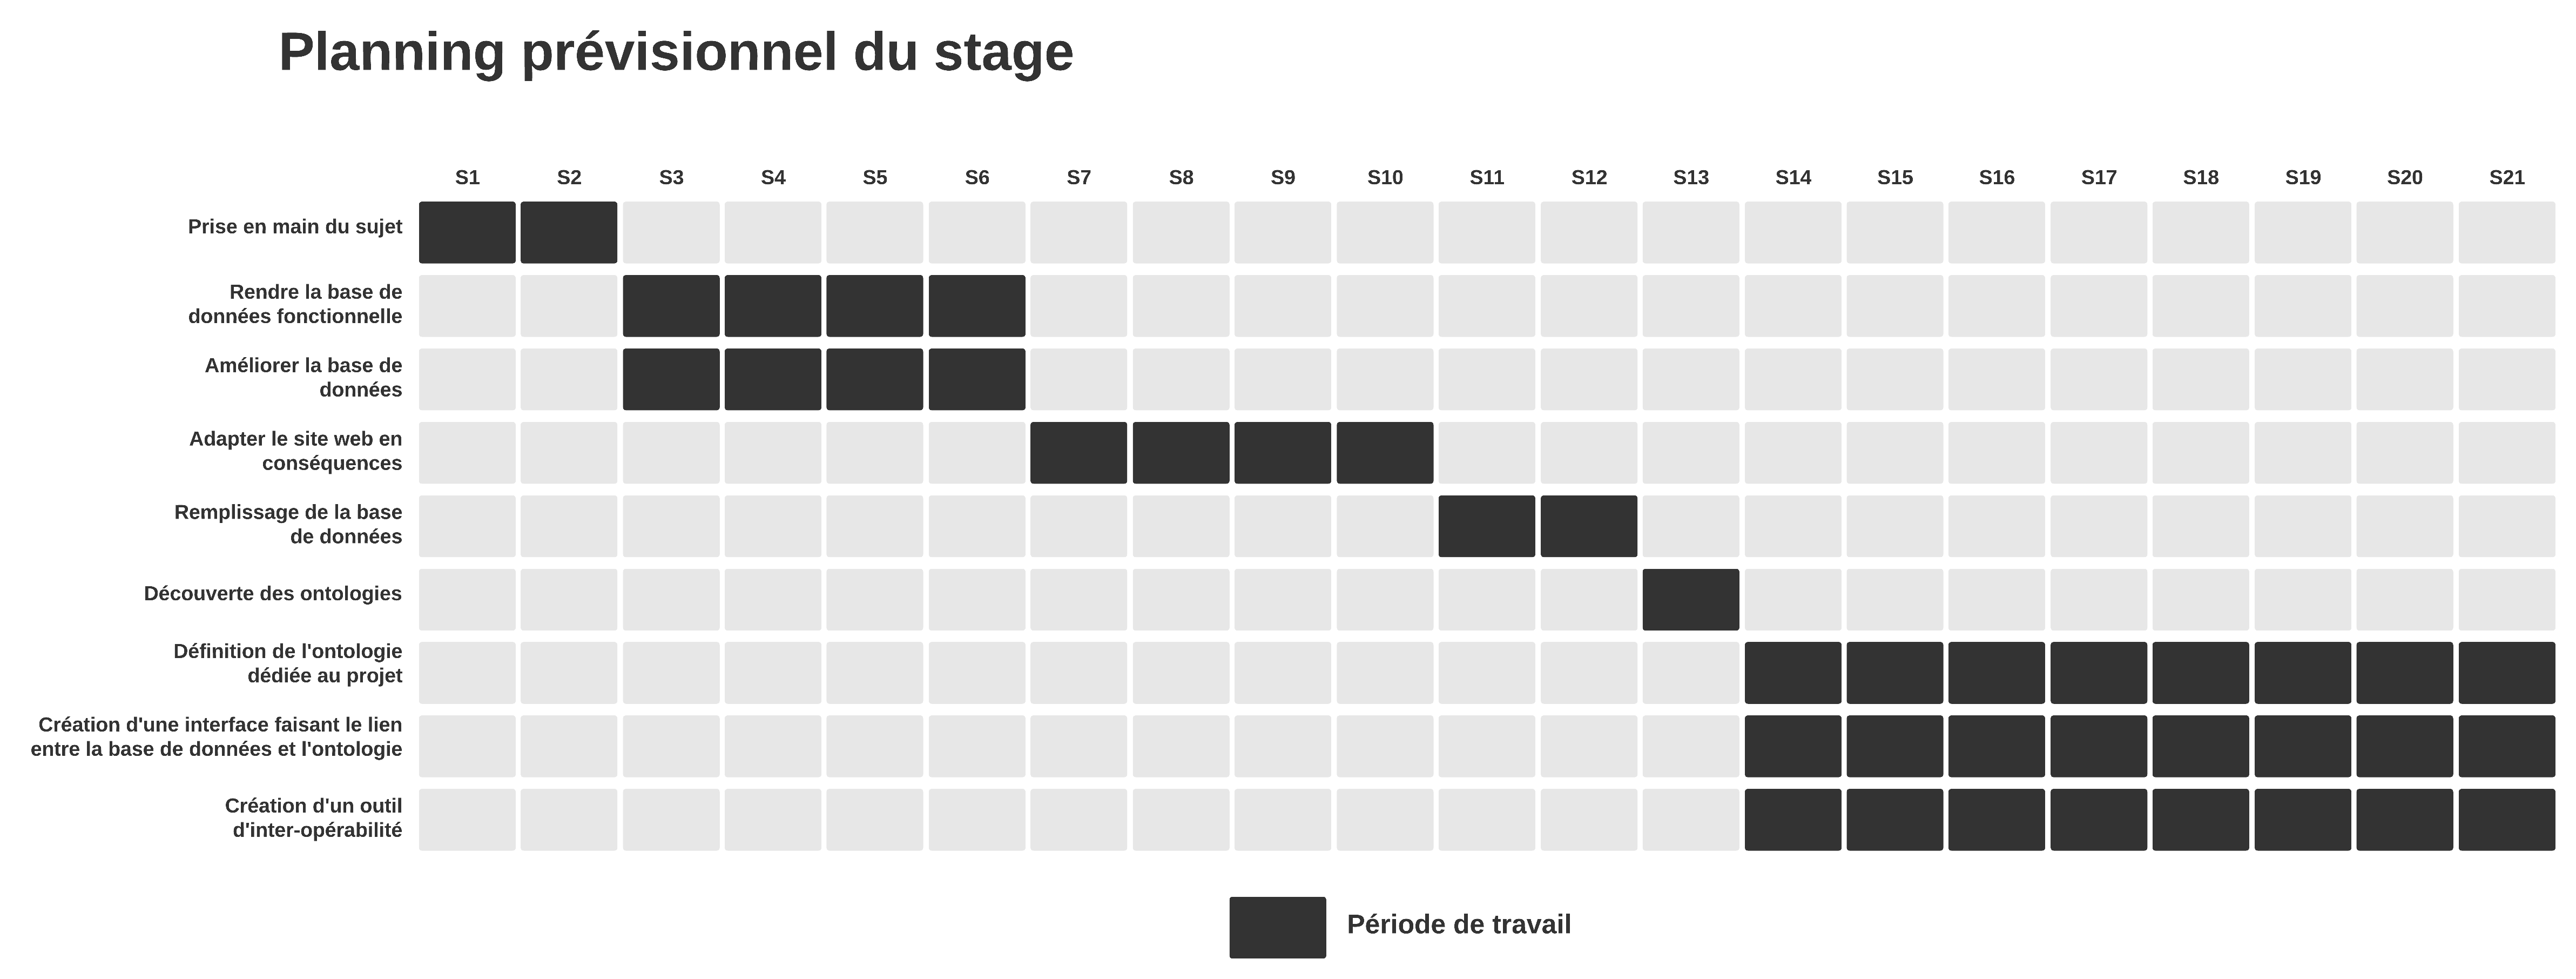
\includegraphics[width=1\textwidth]{assets/planning/planning_previsionnel.png}
    \caption{Planning prévisionnel}
    \label{fig:planningPrevisionnel}
\end{figure}

\section{Planning réel}

\paragraph{} \hspace{10mm}
En comparaison avec ce qui était prévu et ce que j'ai réellement pu faire, voici les plannings réels à la période de Noël et à la fin du stage. Après mon séjour à Nantes pour rencontrer Matthieu Quantin et Florent Laroche, nous avons réalisé que le projet existant posait de nombreux problèmes et qu'il était nécessaire de changer de voie. Nous avons dû corriger notre approche pour gérer le stockage des données liées au projet et cela a entraîné des modifications importantes dans le planning initial.

\begin{figure} [H]
    \centering
    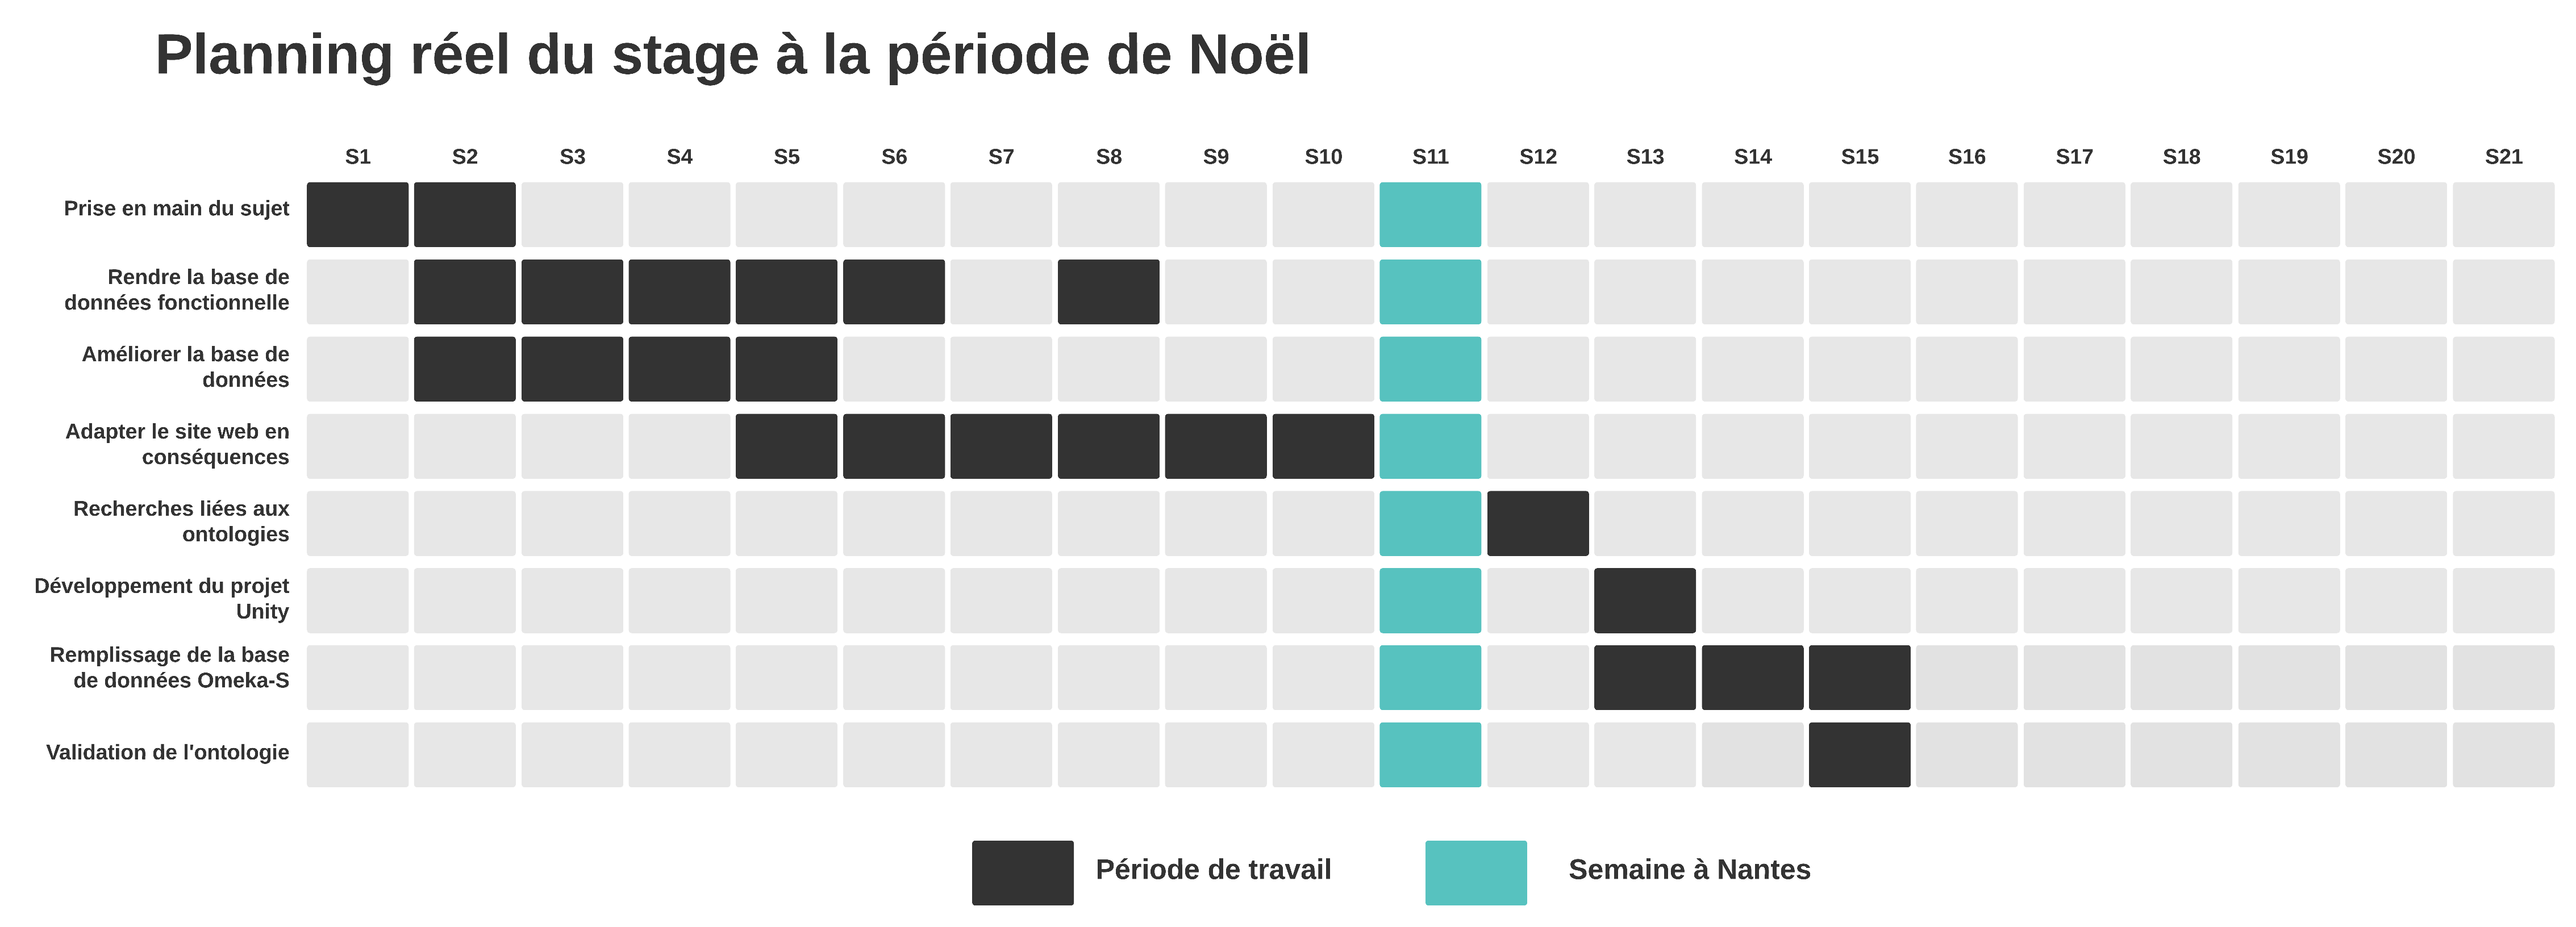
\includegraphics[width=1\textwidth]{assets/planning/planning_reel_noel.png}
    \caption{Planning réel à la période de Noël}
    \label{fig:planningReelNoel}
\end{figure}

\begin{figure} [H]
    \centering
    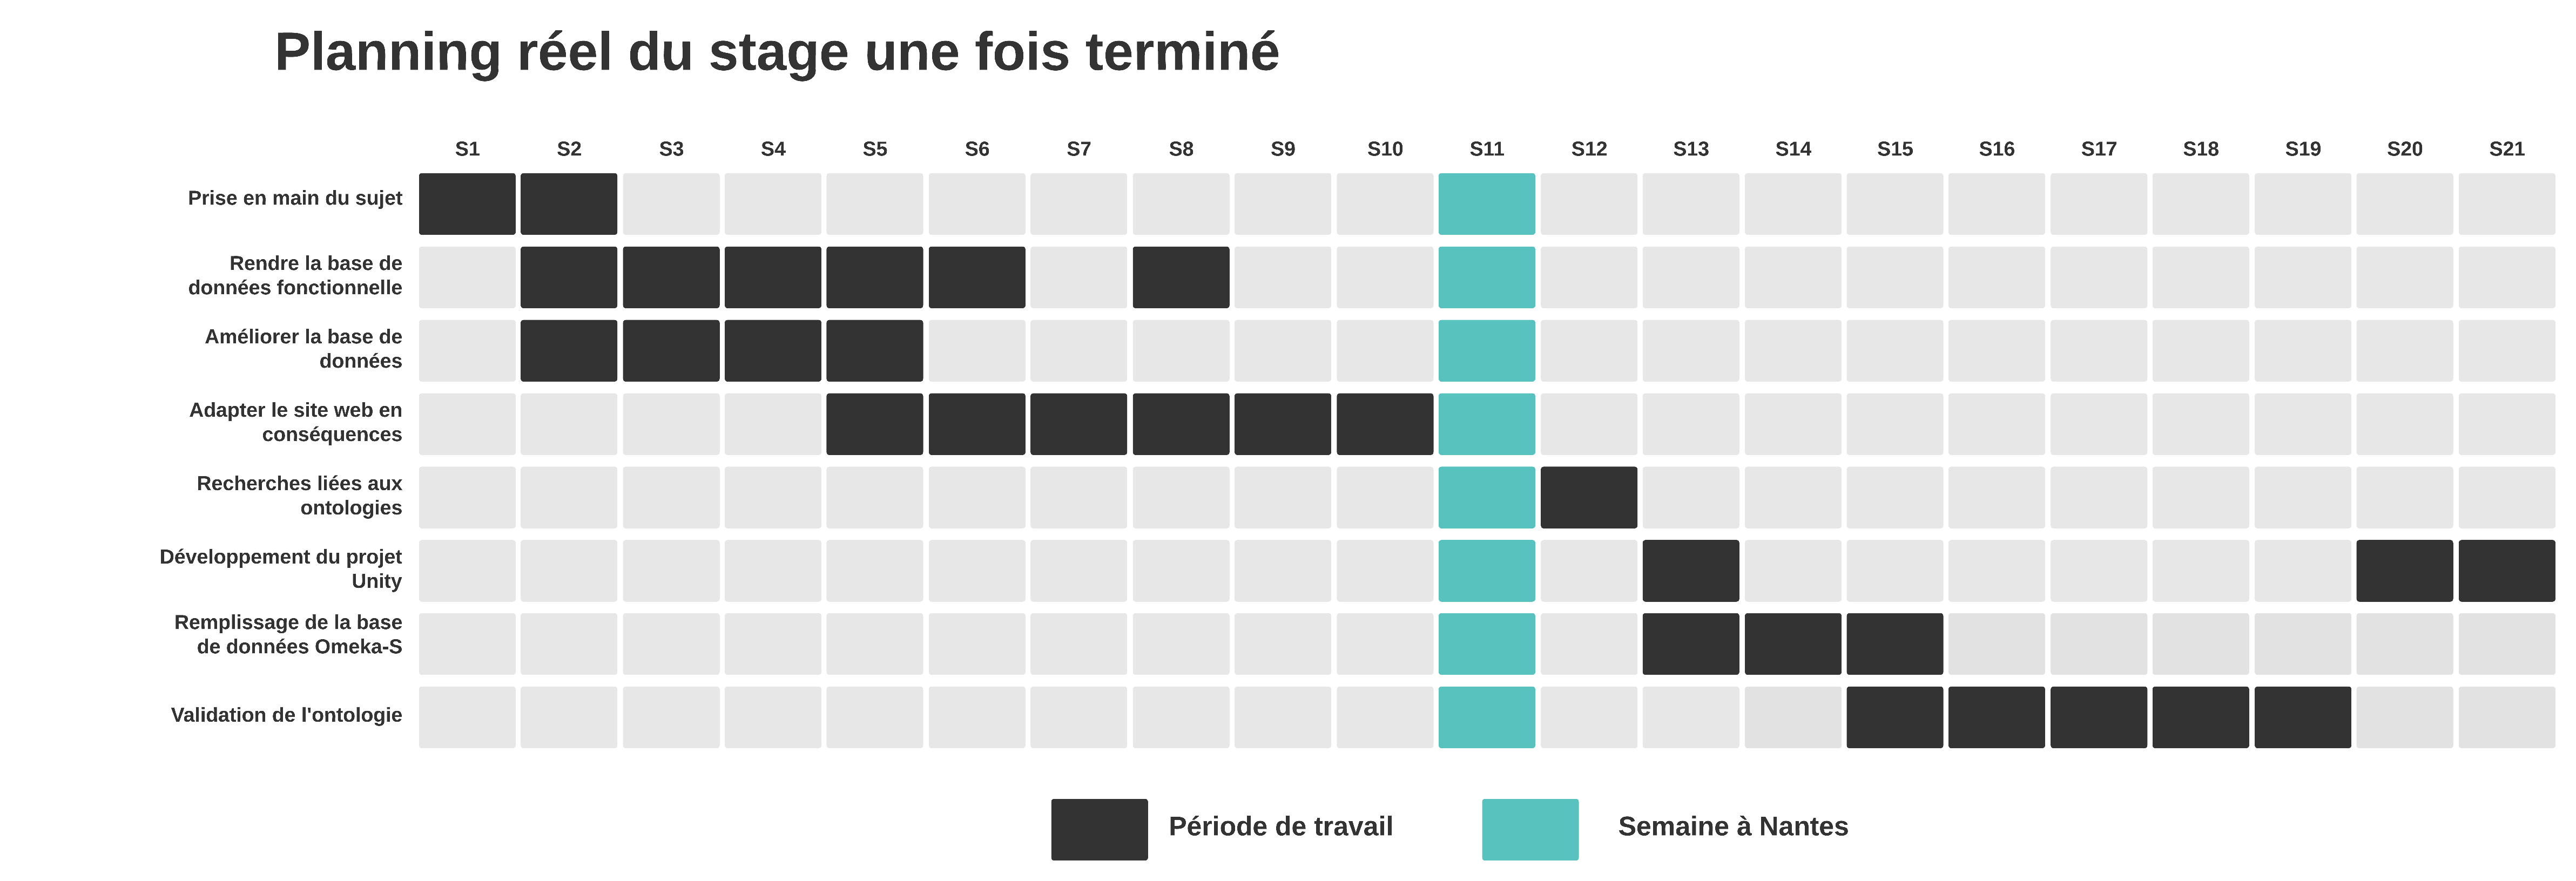
\includegraphics[width=1\textwidth]{assets/planning/planning_fin.png}
    \caption{Planning réel du stage une fois terminé}
    \label{fig:planningFin}
\end{figure}


    \chapter{Techn'hom Time Machine}

\section{Sujet de stage}
\subsection{Sujet initial}
\paragraph{} \hspace{10mm}
Le sujet de stage proposé consistait à enrichir et mettre en place des outils de manipulation de \textbf{la base de données TTM}. Cela incluait l'ajout de nouvelles données et la création de requêtes spécifiques.

Ensuite, nous devions définir les ontologies sous \textbf{OntoMe} et les stocker sous \textbf{Omeka-S}. Cela impliquait la création de modèles de données structurés pour représenter les concepts et les relations entre eux.

Une partie importante de ce stage était la mise en place d'une interface permettant de faire le lien entre la TTM BDD existante et les ontologies. Cela nécessitait une formalisation précise des données et des relations entre elles.

Enfin, nous devions mis en place un protocole d'échanges entre les outils TTM et Omeka-S afin de rendre ces outils inter-opérables. Cela aurait permis de faciliter l'intégration des données et de rendre les outils plus efficaces dans leur utilisation.
\subsection{Sujet réel}
\paragraph{} \hspace{10mm}
Le sujet réel a porté dans un premier temps sur l'amélioration de la base de données existante et du site web. Cela a impliqué l'optimisation des formulaires et l'ajout de fonctionnalités pour faciliter l'utilisation du site ainsi que l'amélioration du modèle relationnel du projet.

En outre, j'ai également travaillé sur la définition d'une ontologie personnalisée basée sur celle du CIDOC-CRM. Cela a été réalisé suite à mon séjour à Nantes, où j'ai pu en apprendre davantage sur les différents concepts et terminologies utilisés dans l'ontologie.

J'ai ensuite validé ce modèle ontologique à l'aide de Protégé et de la spécification SHACL et effectué la première saisie de données.

Enfin, j'ai réalisé une représentation en 3D sous Unity d'un flux à l'aide des données saisies via l'API d'Omeka-S.
\pagebreak
\section{Le projet déjà existant}
\paragraph{} \hspace{10mm}
A mon arrivée en Septembre, le projet avait déjà été amorcé par deux étudiants, \textbf{Gabriel Garcia} et \textbf{Guillaume Ruff}. Le premier à avoir travaillé sur le projet est Gabriel lors de son stage ST40, et est à l'origine de la base de donnée déjà existante ainsi que d'une interface web réalisée avec le framework Vue.js. Guillaume quant à lui, a recréé le site web dans le cadre d'une UV HEDT avec le framework Angular, afin d'avoir un site plus robuste et facile à maintenir.
La première phase du stage a donc consisté à finaliser ces deux projets en vue d'avoir une application web fonctionnelle et avec des interfaces abouties.

\subsection{Le backend : Django}

\setcounter{secnumdepth}{3}
\subsubsection{Présentation et avancement au début du stage}
\paragraph{} \hspace{10mm}
Lors de son stage, Gabriel a travaillé sur le développement d'un modèle relationnel sur le framework Django. Le modèle est divisé en deux sous-modèles : \textbf{Community} et \textbf{Database}. Le premier permet de gérer les utilisateurs, leurs droits et leurs identifiants et le deuxième permet de gérer tout ce qui est lié aux données. 

Le sous-modèle "Community" était déjà fonctionnel et achevé au début du stage : il permet d'avoir toutes les informations nécessaires sur les utilisateurs.

\begin{figure} [H]
    \centering
    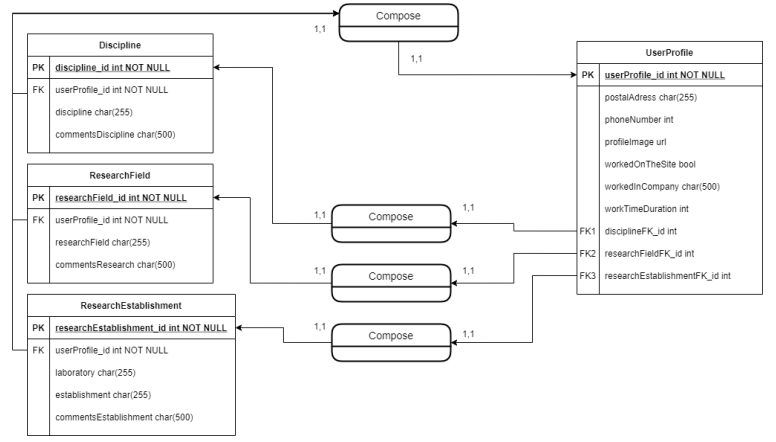
\includegraphics[width=1\textwidth]{assets/web/diagramme_modele_community.png}
    \caption{Diagramme de classe du sous-modèle relationnel "Community"}
    \caption*{\textbf{Source :} Gabriel Garcia}
    \label{fig:diagrammeClasseCommunity}
\end{figure}

\paragraph{} \hspace{10mm}
En revanche, en ce qui concerne la partie \textbf{Database}, tout n'était pas fonctionnel et terminé. Tout d'abord, nous avons très vite remarqué des problèmes de normalisations, qu'elles soient relationnelles ou syntaxiques. En témoigne la capture d'écran suivante, il y avait par exemple la table \textbf{Date} qui avait certains de ses champs dupliqués :

\begin{figure} [H]
    \centering
    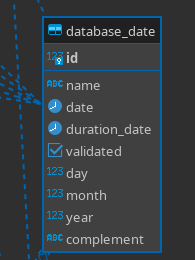
\includegraphics[width=0.175\textwidth]{assets/web/table_date.png}
    \caption{Capture d'écran de la table date du diagramme de classe du sous-modèle "Database"}
    \label{fig:tableDateDatabase}
\end{figure}

Comme on peut le voir, la table se compose d'un champ "date" de type Date ainsi que de trois champs "day", "month" et "year" de type Nombre. Les trois champs de type Nombre sont complètement inutiles et par conséquent la base de données ne respecte pas la forme normale 1FN.

Outre l'absence de forme normale du modèle, le code n'était lui non plus pas normalisé : certains champs des tables étaient déclarés en \textbf{Lower camel case}, et d'autres en \textbf{Upper camel case} ou en \textbf{Snake case}.

Enfin, les tests écrits par Gabriel relevaient 27 erreurs dont 22 liées à la table "source" ou à la table "source type".

\paragraph{} \hspace{10mm}
Dans l'ensemble l'essentiel du travail avait déjà été réalisé, comme on peut le voir ci-après même si tout n'est pas parfait. Dans un premier temps, notre tâche a été de tout normaliser et de "lisser" le code afin de le rendre plus clair. Ensuite, l'absence d'historien pour aider Gabriel s'est aussi faite sentir lorsque Cyril Lachèze est arrivé : dès les premières réunions nous avons vu que l'état dans lequel était le modèle ne permettrait pas d'enregistrer des données avec une granularité (i.e. le niveau de précision) convenable. Il fallait donc que l'on trouve une solution pour cela.

\begin{figure} [H]
    \centering
    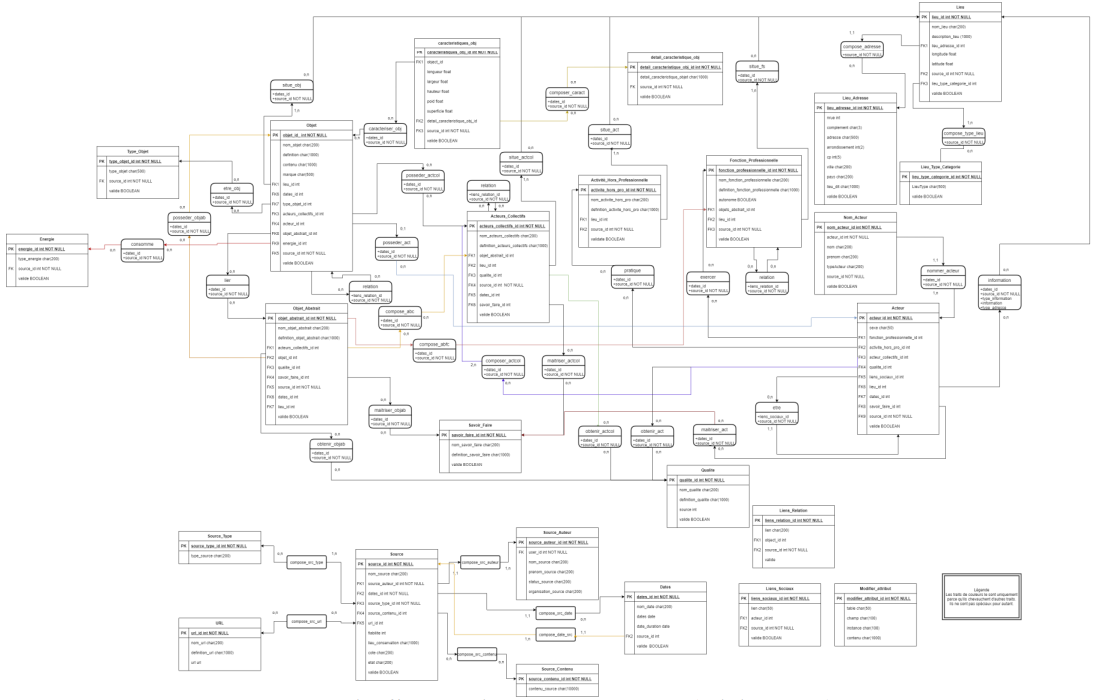
\includegraphics[width=1\textwidth]{assets/web/diagramme_modele_database.png}
    \caption{Diagramme de classe du sous-modèle relationnel "Database"}
    \caption*{\textbf{Source :} Gabriel Garcia}
    \label{fig:diagrammeClasseDatabase}
\end{figure}

\subsubsection{Le travail à effectuer}
\paragraph{} \hspace{10mm}
Pour rendre la base de données fonctionnelle, nous avons effectué plusieurs tâches clés. Tout d'abord, nous avons corrigé les bugs affectant les tables "source" et "source type". Ces bugs nous ont posés beaucoup de difficultés, qui peuvent être expliquées par trois facteurs :
\begin{itemize}
    \item[\ding{103}] premièrement, les migrations effectuées tout au long du développement du modèle étaient "corrompues". Au fil des modifications de ces deux tables, des coquilles se sont insérées dans le code des migrations ce qui les empêchaient de bien s'appliquer, résultant de l'apparition d'erreurs.
    \item[\ding{103}] deuxièmement, le champ liant la table "source type" à la table source était mal déclaré, ce qui a décuplé notre incompréhension vis-à-vis des erreurs si l'on prend en compte le premier point.
    \item[\ding{103}] enfin, ma non-maîtrise de django au début du stage et mon manque d'expérience en tant que développeur m'ont fait perdre beaucoup de temps. Connaissant mal le framework, j'ai par exemple mis plusieurs jours avant de comprendre l'intérêt du fichier \textbf{admin.py} et celui de dé-commenter la ligne qui ajoutait la table "source" au panneau d'administrateur, ce qui m'a par la suite beaucoup aidé à débugger les erreurs.  
\end{itemize}
\paragraph{} \hspace{10mm}
Ensuite, nous avons dû revoir les noms des champs avec Cyril. Ceux-ci n'étaient pas toujours explicites (voire pas du tout) et leur utilité n'était pas systématiquement expliqué dans le rapport de stage de Gabriel, il fallait donc les modifier (la figure 3.2 est un bon exemple : à ce jour, je n'ai toujours pas très bien compris l'intérêt du champ "duration\_date"). Cyril avait commencé à travailler sur ce sujet mais mon séjour à Nantes l'a interrompu suite à l'abandon de la base.
\paragraph{} \hspace{10mm}
En parallèle, nous avons également corrigé les erreurs dans les tests unitaires qui nous ont menés à une compréhension erronée du fonctionnement. Certains fonctionnent de nouveau mais il y a encore 5 tests défaillants : ils retournent une erreur alors qu'en pratique tout fonctionne. Nous n'avons pas réussi à les corriger, par conséquent nous les avons laissé tels quels et nous avons ajouté un commentaire dans le code indiquant qu'il fallait ignorer l'erreur.

\subsection{Le frontend : Angular (et Vue.Js)}

\subsubsection{Présentation et avancement au début du stage}
\paragraph{} \hspace{10mm}
Lorsque mon stage a débuté en septembre, deux interfaces avaient été conçues sous la forme de sites web. La première, implémentée par Gabriel, utilisait le framework \textbf{Vue.Js} et n'était pas totalement achevée : la structure globale du site était fonctionnelle mais les formulaires n'étaient pas exactement terminés et de nombreux petits détails pouvaient être corrigés afin d'améliorer l'expérience utilisateur.

\begin{figure} [H]
    \centering
    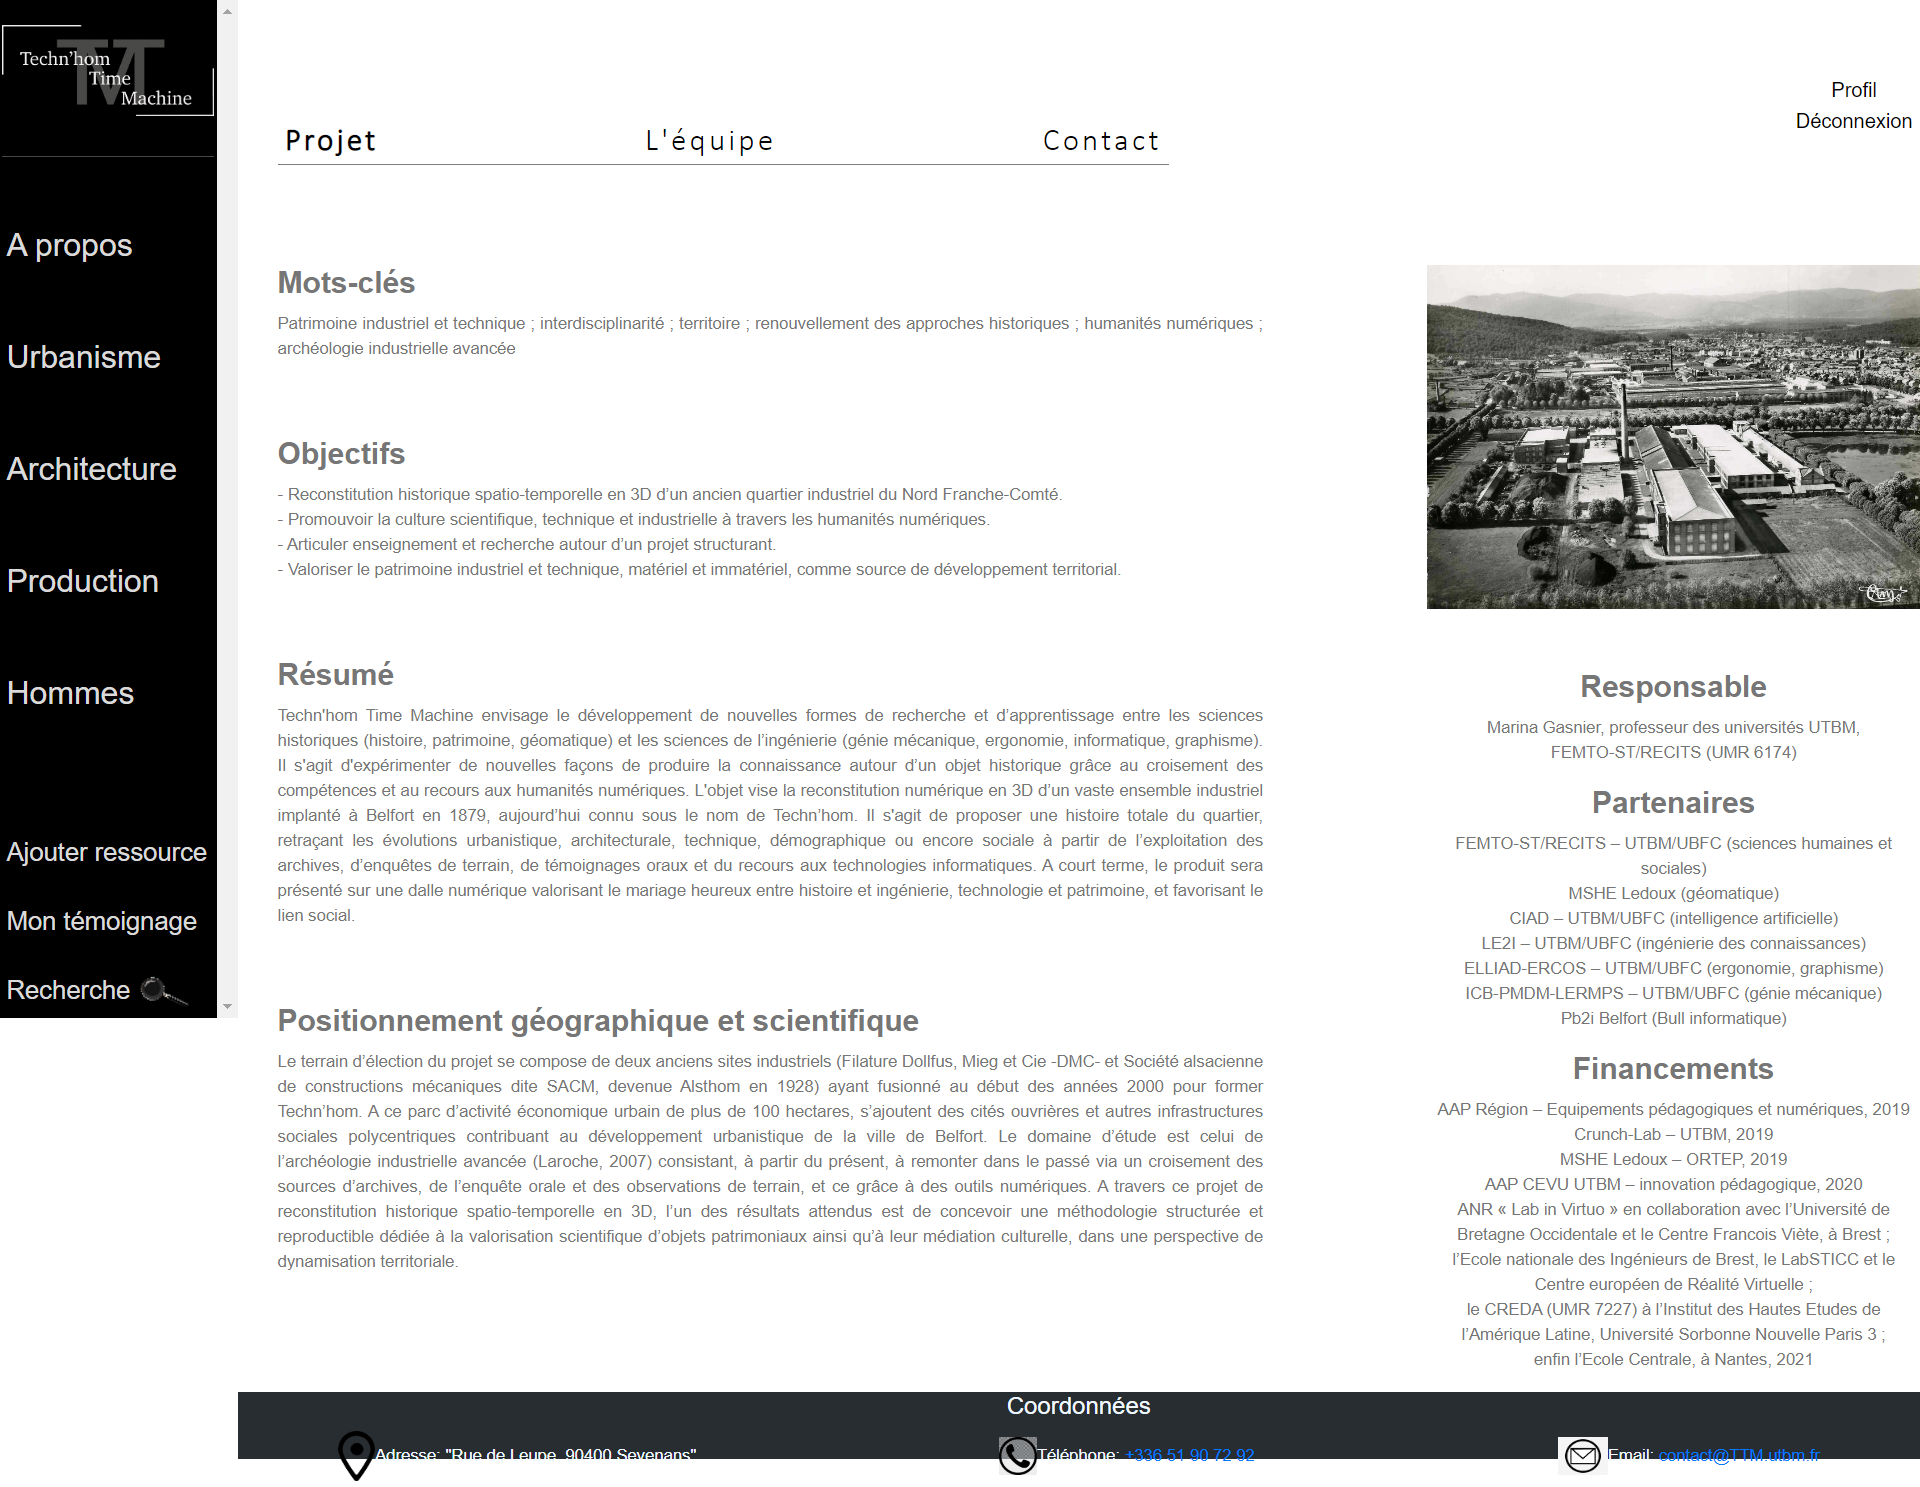
\includegraphics[width=1\textwidth]{assets/web/screen_main_vue.png}
    \caption{Capture d'écran de la page "A Propos" du site réalisé en Vue.Js}
    % \caption*{\textbf{Source :} Gabriel Garcia}
    \label{fig:screenMainVue}
\end{figure}

\Note{Le screenshot étant effectué avec une extension chrome qui "déroule" la page pour tout voir, on ne peut en fait pas tout lire sans défiler et le bandeau de gauche n'est pas trop petit}

\paragraph{} \hspace{10mm}
Nous pouvons voir sur cet exemple que plusieurs aspects peuvent être améliorés, comme les boutons \textbf{Profil} et \textbf{Déconnexion} qui ne sont pas très esthétiques ni très bien disposés. Le pied de page pourrait également être mieux façonné, tant sur la qualité des icônes que sur l'alignement du texte.

\paragraph{} \hspace{10mm}
Suite au stage de Gabriel, c'est ensuite Guillaume qui a poursuivi le projet au travers de l'UV HN2B. Son objectif tout au long du semestre avait été de recréer le site avec le framework \textbf{Angular}, Vue.Js ayant été jugé moins stable et moins maintenable. Ici aussi, Guillaume n'a pas pu achever son travail : aucune interface permettant d'afficher les données ni aucun formulaire n'avait été réalisé, il fallait donc tout designer et implémenter pour que l'ensemble soit opérationnel.

Voici à titre de comparaison la page "A propos" du site de Guillaume : 
\begin{figure} [H]
    \centering
    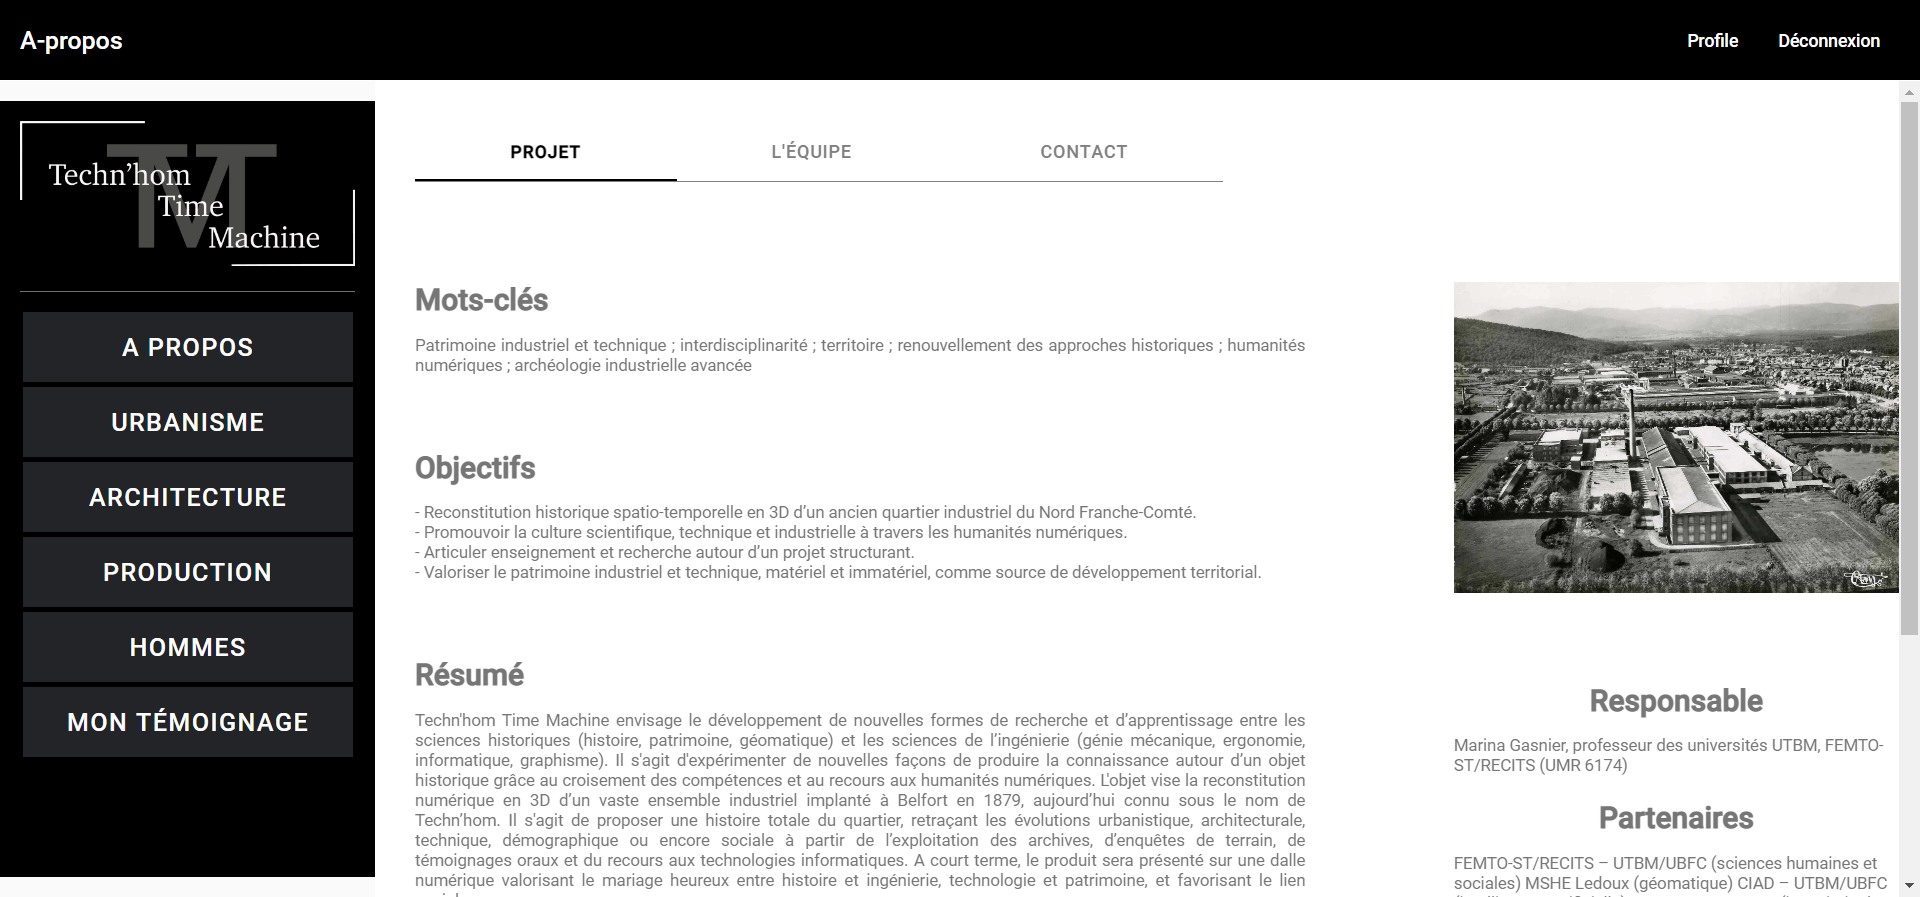
\includegraphics[width=1\textwidth]{assets/web/screen_main_angular.png}
    \caption{Capture d'écran de la page "A Propos" du site réalisé en Angular}
    % \caption*{\textbf{Source :} Gabriel Garcia}
    \label{fig:screenMainAngular}
\end{figure}

\subsubsection{Le travail à effectuer}
\paragraph{} \hspace{10mm}
Afin de finir le site, nous avons dû terminer deux tâches importantes : designer et implémenter les formulaires de saisies de données ainsi que les interfaces pour afficher ces mêmes données. Contrairement à Gabriel, nous n'avons pas souhaité utiliser Figma au vu de ce qu'il a pu en dire dans son rapport : ne sachant pas utiliser le logiciel et Figma ne permettant pas d'extraire du code HTML de bonne qualité, nous avons préféré designer nous-même interfaces et formulaires en se basant sur ce qui avait déjà été fait, c'est-à-dire, reproduire (dans un premier temps au moins) les formulaires de Gabriel tels quels tout en appliquant le nouveau style UI de Guillaume.

Pour plus d'efficacité, nous avons pensé que tout implémenter pour une des trois sections (Architecture, Production, Hommes) avant de passer à la section d'après était une meilleure idée que de créer tous les formulaires puis toutes les interfaces d'affichage, car cela nous éviterait d'avoir à effectuer trois fois les mêmes modifications en cas d'imprévu dans le design de ceux-ci. 

\paragraph{} \hspace{10mm}
La première (et unique) section que nous avons commencé à traiter est la section "Hommes". Dans un premier temps, nous avons pensé l'interface générale d'affichage des données puis l'interface d'affichage des détails. Seule la page affichant la liste des acteurs est terminée, mon séjour à Nantes ayant interrompu le développement du site, comme on peut le voir sur les figures 3.6 et 3.7 ci-après.

Par ailleurs, pour les mêmes raisons, aucun formulaire n'a pu être ébauché.
\begin{figure} [H]
    \centering
    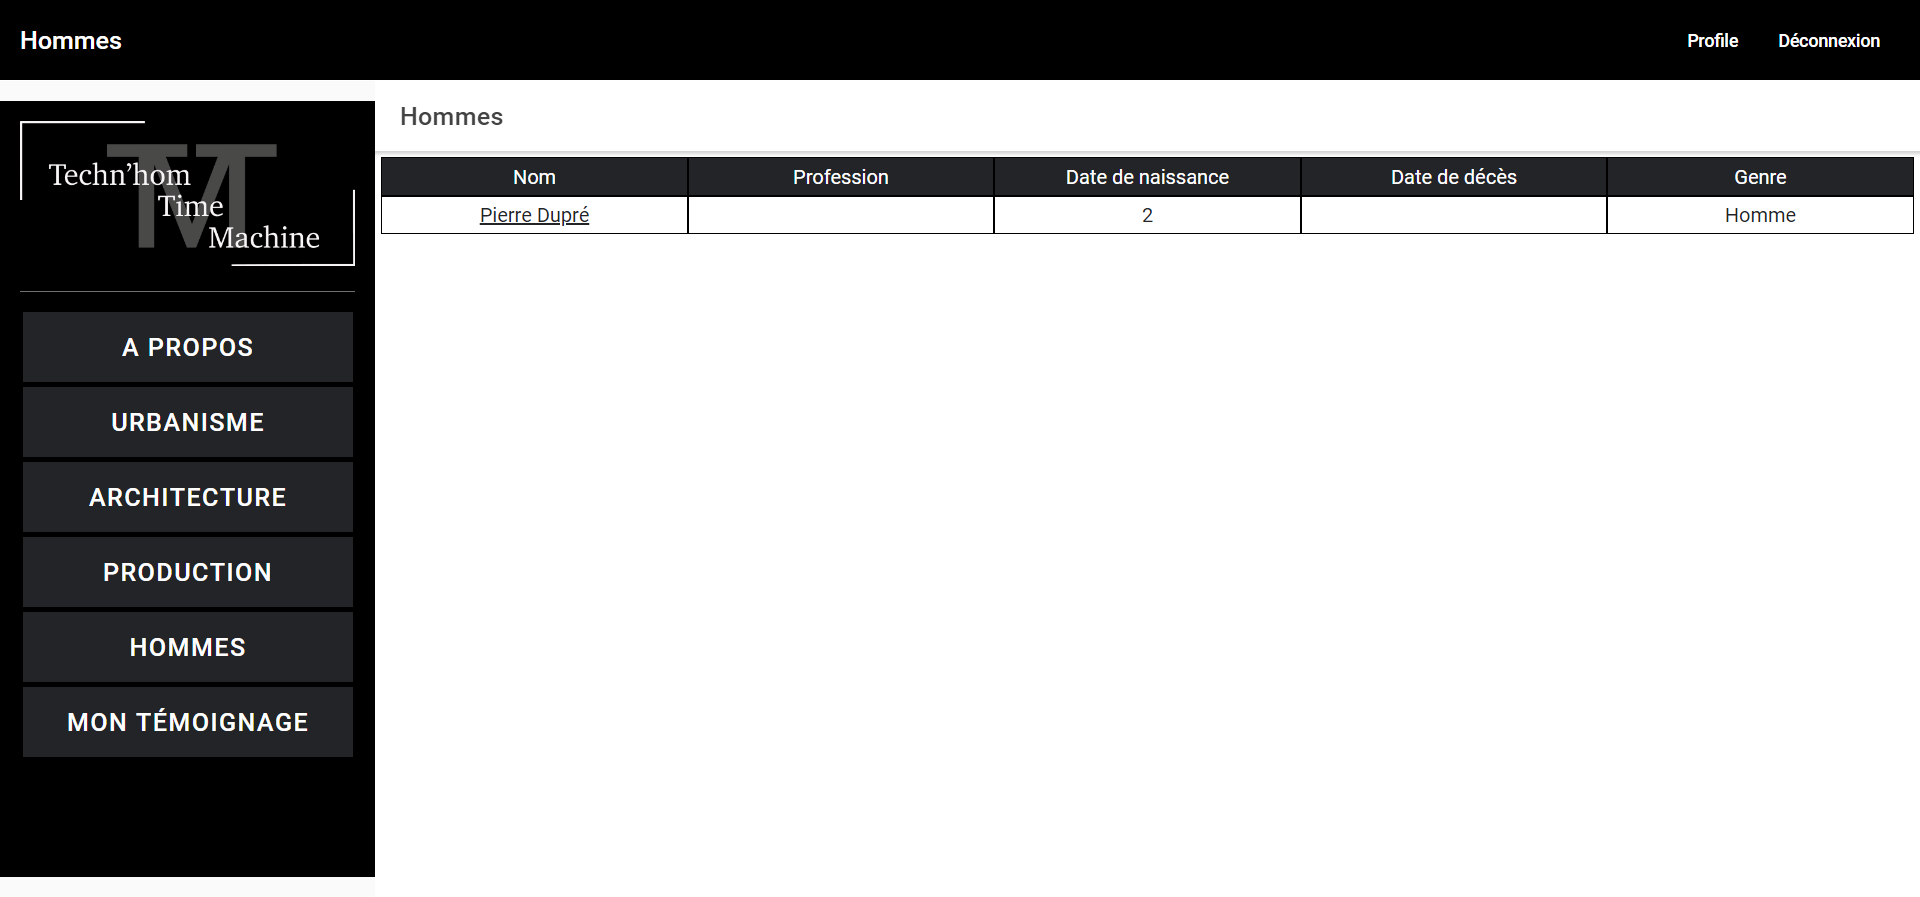
\includegraphics[width=1\textwidth]{assets/web/site/screen_liste_hommes.png}
    \caption{Capture d'écran de la page "Hommes" du site affichant les Acteurs}
    \label{fig:screenPageHommes}
\end{figure}

\begin{figure} [H]
    \centering
    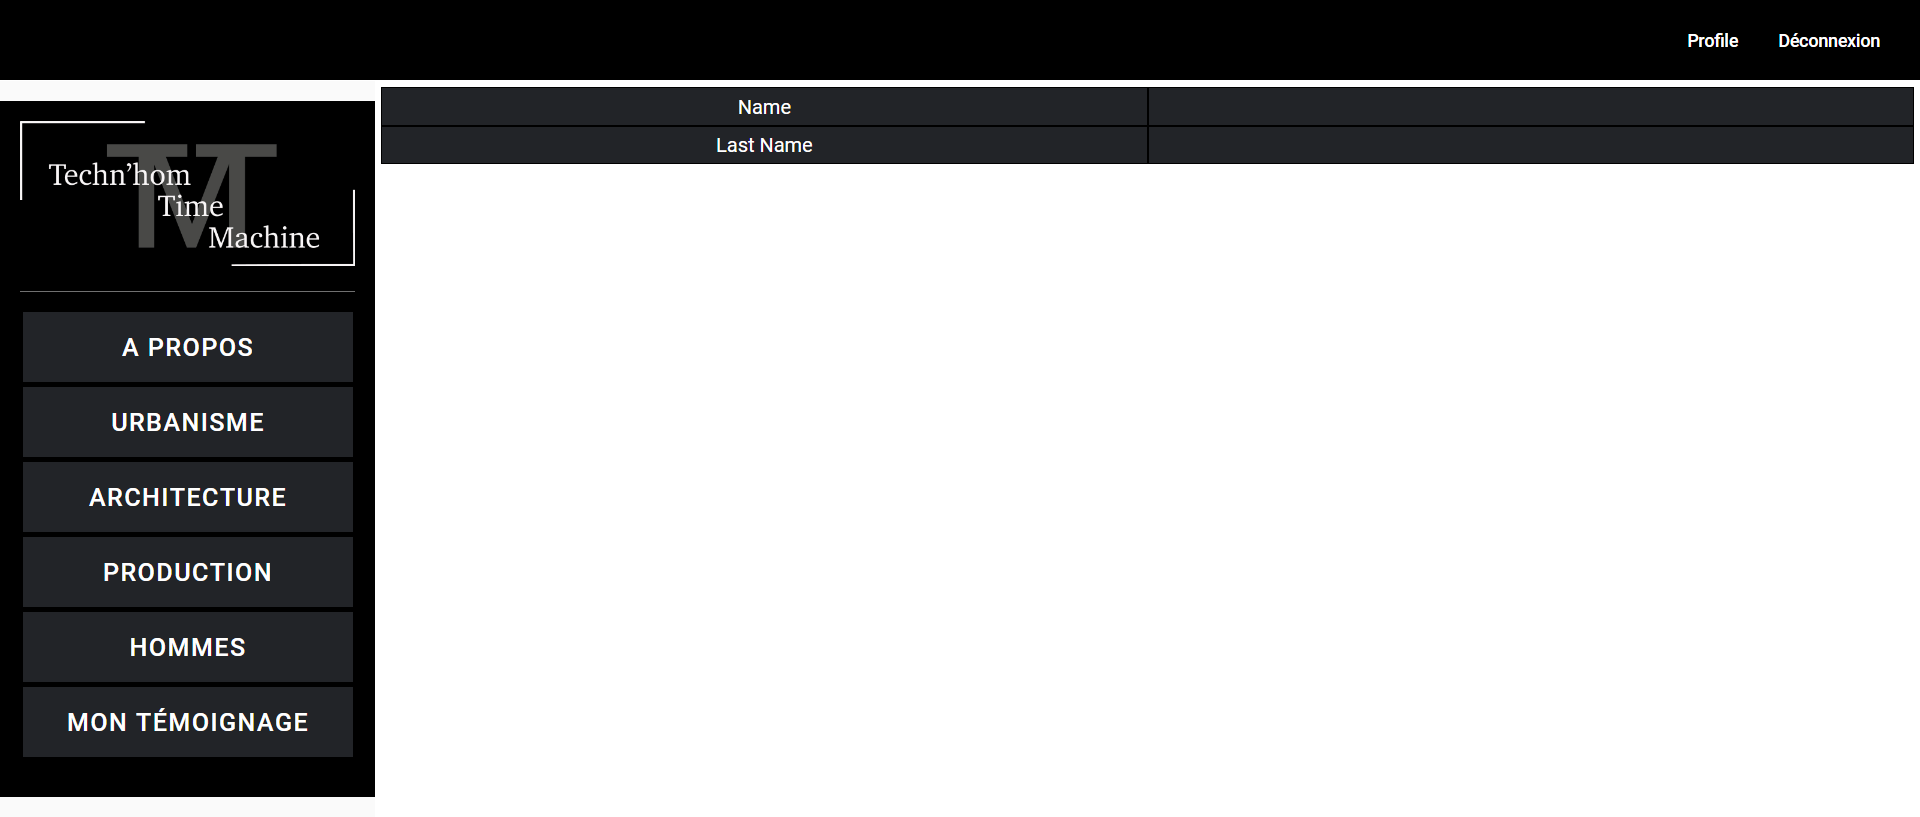
\includegraphics[width=1\textwidth]{assets/web/site/screen_detail_hommes.png}
    \caption{Capture d'écran de la page de détail d'un des acteurs de la page "Hommes"}
    \label{fig:screenPageHommesDetails}
\end{figure}

\pagebreak
\subsection{Problématique rencontrée}

\paragraph{} \hspace{10mm}
Pendant la semaine du 7 novembre, nous avons pris conscience que certains éléments ne convenaient pas dans le projet dans son état actuel. 

Tout d'abord, le modèle de la base de données n'était pas aussi abouti que nous le pensions. L'inconvénient d'un modèle relationnel (comparé à un modèle ontologique que nous aborderons après), est qu'il est beaucoup trop rigide pour le projet. Par conséquent, pour enregistrer par exemple deux objets qui ont des caractéristiques communes et des caractéristiques qui leur sont propres, nous avons deux solutions : soit créer une table commune aux deux avec tous les champs nécessaires, soit créer deux tables distinctes. Le problème de la première est son manque de "propreté" : ce n'est pas pratique d'utiliser une telle méthode car cela créerait des formulaires à rallonge dont la plupart des champs ne serviraient pas à chaque fois. Quant à la seconde, elle est mauvaise également car cela impliquerait de créer un nombre colossal de tables, ce qui n'est pas viable. Au final, aucune solution de convient pour un problème aussi basique.

Ensuite, les formulaires posaient aussi problème. Après avoir analysé le code de Gabriel, nous avons remarqué qu'il nous était impossible par exemple de lier plusieurs objets d'une certaine table à un objet d'une autre table à cause de la séparation du site en trois parties (Hommes, Architecture, Production).

Enfin, contrairement à ce qui était prévu dans le sujet de stage, il n'existe aucun outil d'échange entre une base relationnelle et Omeka-S. Par conséquent, il aurait fallu en créer un ce qui aurait pris beaucoup trop de temps et ne m'aurait pas permis d'atteindre mes objectifs de fin de stage. La seule autre option pertinente aurait été un triple-store, mais cela ne correspondait pas non plus au sujet initial.

Fort heureusement, mon séjour à Nantes a provoqué un tournant et nous avons pu repartir sur de nouvelles bases pour le projet grâce à Matthieu Quantin et l'utilisation des vocabulaires ouverts liés, aussi appelés ontologies.

\pagebreak
\section{Création de la base de données ontologique}
\subsection{L'ontologie du projet}

\subsubsection{Les ontologies : la théorie}
\paragraph{} \hspace{10mm}
Une ontologie informatique est un modèle conceptuel qui décrit les concepts et les relations qui existent dans un domaine d'application spécifique. Elle sert à fournir une structure de données commune pour les systèmes informatiques qui traitent ces données. Les ontologies informatiques sont généralement définies en utilisant un formalisme de description de la connaissance, comme OWL (Web Ontology Language) ou RDF (Resource Description Framework). Elles peuvent être utilisées pour des tâches comme la classification automatique, la recherche d'information, la reconnaissance de la parole, la compréhension de la langue naturelle, et la communication entre systèmes informatiques.
Elles sont utilisées pour fournir un cadre commun pour les systèmes informatiques pour comprendre et partager l'information. Cela permet de faciliter la communication entre les systèmes et d'améliorer l'interopérabilité entre différents systèmes. Elles sont également utilisées pour améliorer la performance des systèmes d'IA en fournissant une description précise et complète des concepts dans un domaine d'application.

\paragraph{} \hspace{10mm}
Cette approche étant plutôt abstraite, on peut la concrétiser en ajoutant que le World Wide Web Consortium a défini un langage appelé OWL (Web Ontology Language) basé sur le standard RDF (Resource Description Framework). RDF est un framework permettant de modéliser des graphes destiné à décrire des ressources web (et leurs métadonnées). Un document suivant la structure RDF est composé de \textbf{triplets} ordonnés de la manière suivante : \textbf{(sujet, prédicat, objet)}.

\begin{itemize}
    \item[\ding{103}] Le \textbf{sujet} est la ressource que l'on souhaite décrire.
    \item[\ding{103}] Le \textbf{prédicat} est la propriété que l'on souhaite appliquer sur le sujet.
    \item[\ding{103}] L'\textbf{objet} est la ressource ou la valeur litérale (nombre, chaine de caractères, URI) que l'on associe au sujet. Autrement dit, c'est la valeur de la propriété.
\end{itemize}

Voici un court exemple résumant l'aspect théorique. Imaginons que l'on veuille représenter des données et métadonnées de la page wikipédia de \href{https://fr.wikipedia.org/wiki/Johann_Joachim_Winckelmann}{Johann Joachim Winckelmann} à l'aide de l'ontologie \textbf{dcterms}, cela pourrait donner les triplets suivants :
            \begin{minted}{turtle}
            @prefix dcterms: <http://purl.org/dc/terms/>
            
            <https://fr.wikipedia.org/wiki/Johann_Joachim_Winckelmann>
                dcterms:title "Johann Joachim Winckelmann ;
                dcterms:publisher <https://fr.wikipedia.org/> ;
                dcterms:issued 2004-10-19 .
            \end{minted}

\subsubsection{Le modèle ontologique}
\paragraph{} \hspace{10mm}
L'ontologie du projet est basée sur plusieurs ontologies différentes afin de couvrir tous les aspects de la description de patrimoine industriel. La principale ontologie utilisée est celle du \textbf{CIDOC-CRM}, car elle est spécifiquement conçue pour décrire des objets et des événements liés au patrimoine industriel. Nous avons également utilisé  \textbf{Bibo} pour représenter les documents, images et autres sources utilisées dans le projet. Pour décrire les liens entre les personnes morales et physiques ainsi que les groupes de personnes, nous avons utilisé les "sous-ontologies" \textbf{rdac} et \textbf{rdaa}, les deux étant intimement liées : la première regroupe les classes de l'ontologie \textbf{RDA} et la seconde les propriétés qui s'appliquent sur ces classes. Nous avons également utilisé \textbf{dcterms} pour décrire les métadonnées des entités bibo. Enfin, nous avons utilisé \textbf{schema} et \textbf{relationship} pour ajouter quelques propriétés supplémentaires qui ne sont pas couvertes par les ontologies cidoc-crm et rdaa. Cette combinaison d'ontologies permet de couvrir l'ensemble des aspects de la description de patrimoine industriel de manière complète et précise. De plus, il est tout à fait possible de greffer de nouvelles ontologies au besoin dans le cas où les ontologies ici décrites ne suffiraient pas à représenter certaines données ou situations.
\paragraph{} \hspace{10mm}
Dans le cadre du projet, nous n'avons pas ajouté de contenu fait par nous-même (classes ou propriétés) ni modifié en profondeur les ontologies existantes. Cela a été fait pour faciliter l'inter-opérabilité avec d'autres systèmes et garder une ontologie la plus proche possible des normes W3C (World Wide Web Consortium). En utilisant des ontologies existantes et en les combinant de manière appropriée, nous avons pu créer une ontologie personnalisée qui répond aux besoins spécifiques de notre projet tout en restant conforme aux normes de l'industrie. Cela a également permis de réduire les risques d'incompatibilité et faciliter la communication et l'intégration future dans d'autres systèmes.

Pour pouvoir faire ceci de la meilleure manière possible, nous avons, avec Cyril Lachèze et Matthieu Quantin, étudié des cas concrets en utilisant des documents fournis par Cyril. Cela nous a aidé à comprendre comment articuler toutes les ontologies et ainsi élaborer une stratégie pour les combiner efficacement en une seule ontologie globale. Cette approche nous a également permis de mieux comprendre les avantages et les limites de chaque ontologie et de prendre des décisions éclairées sur la façon de les utiliser.

\paragraph{} \hspace{10mm}
Afin de pouvoir dresser le schéma de l'\underline{\hyperref[annexe1]{annexe 1}}, nous avons utilisé des images de l'usine SACM de Belfort que Cyril avait à sa disposition. L'intérêt d'utiliser des cas concrets est que l'on peut couvrir et imaginer comment représenter certains cas d'utilisation que l'on n'aurait pas pu imaginer seul.

\begin{figure} [H]
    \centering
    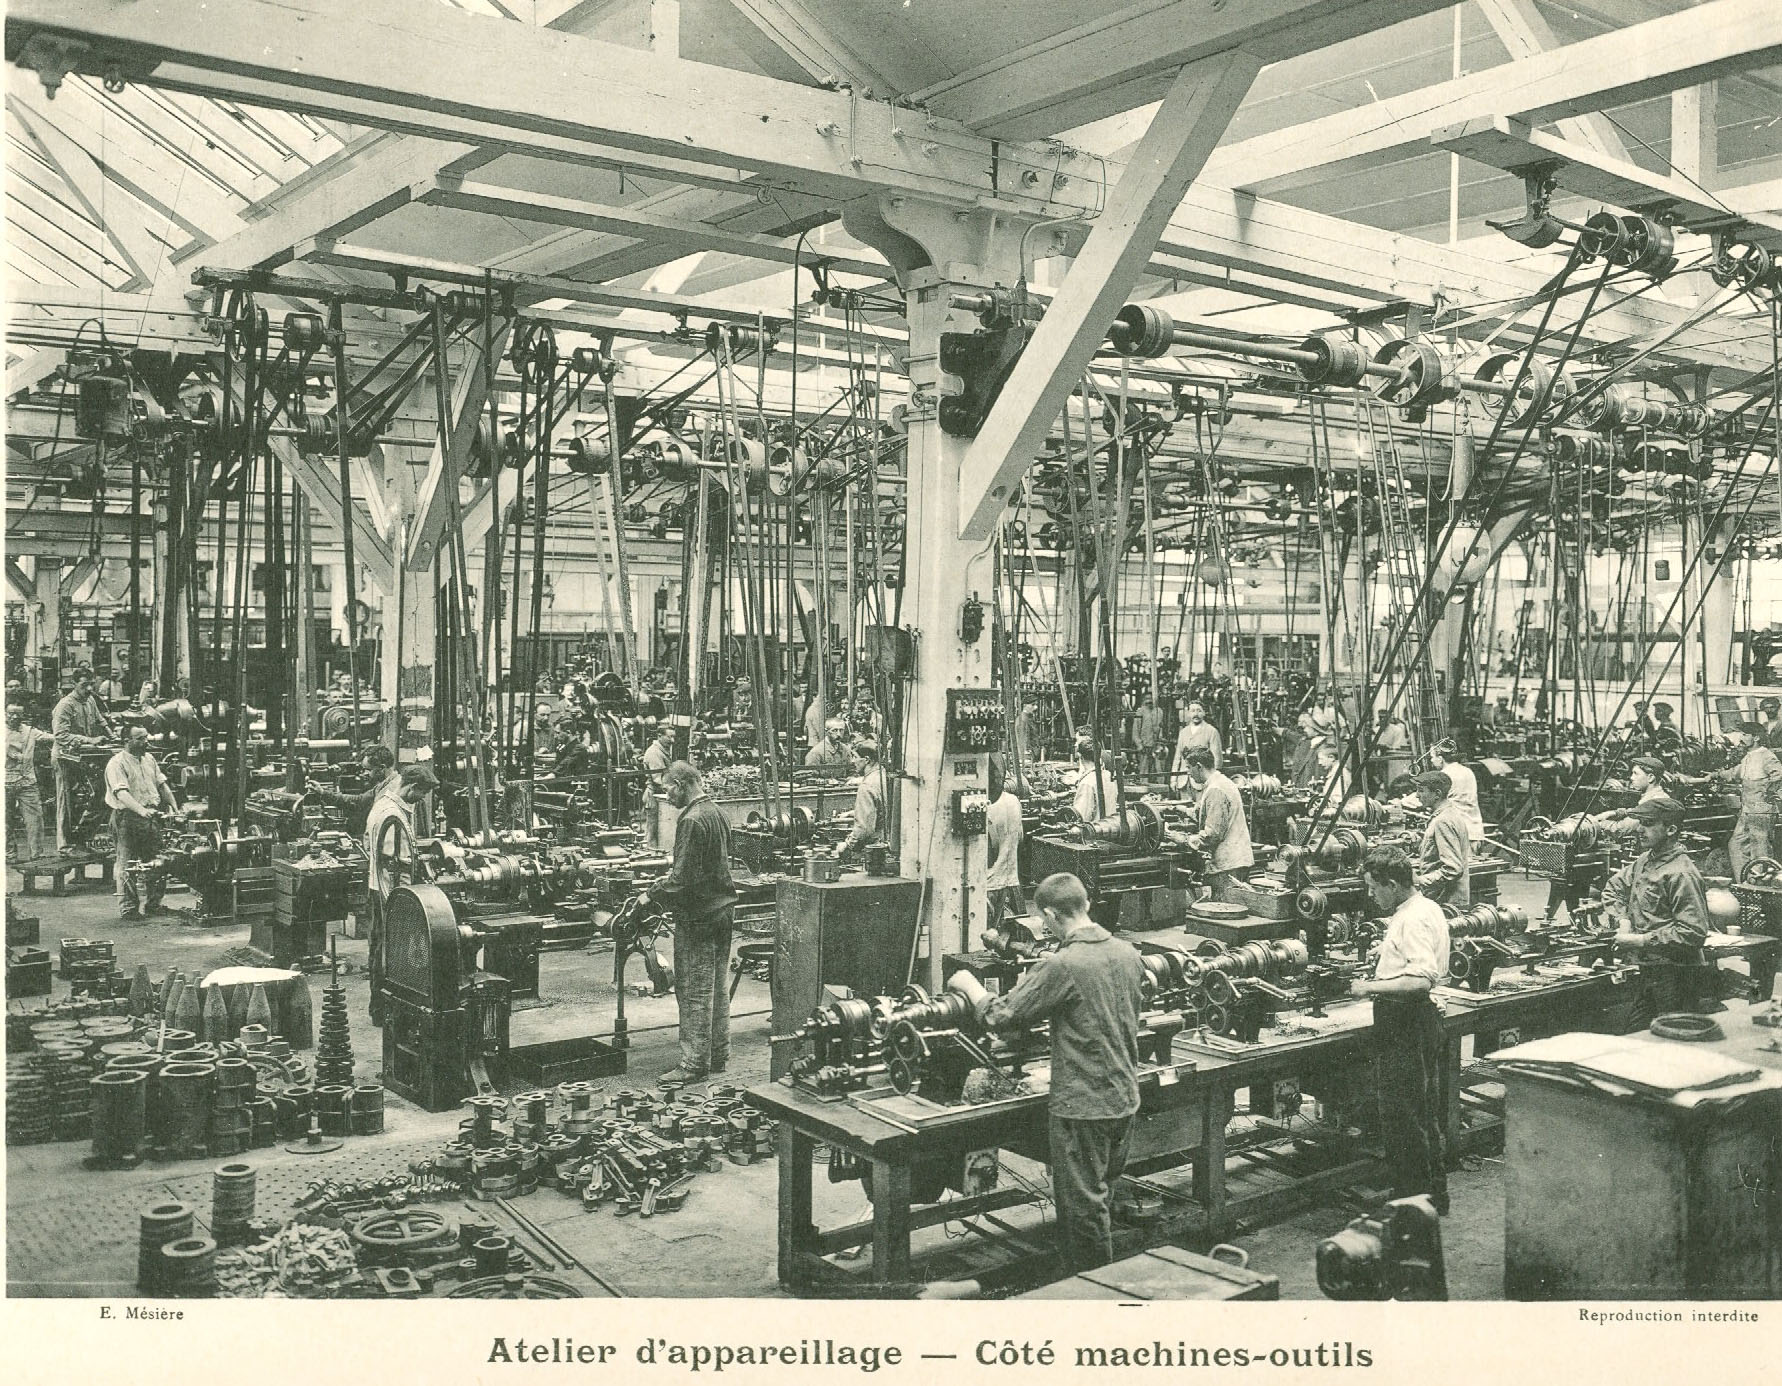
\includegraphics[width=1\textwidth]{assets/ontologie/Atelier d'appareillage - côté machines outils.jpg}
    \caption{Image utilisée afin de dresser le premier schéma expliquant les articulations entre les différentes ontologies}
    \label{fig:photoInspiSchemaBase}
\end{figure}

\paragraph{} \hspace{10mm}
L'ensemble de l'ontologie est centrée sur celle du \textbf{CIDOC-CRM}. Pour pouvoir suivre les normes de l'industrie, nous nous sommes fixés certaines règles à suivre qui permettent deux choses : premièrement, cela facilite l'alignement de notre ontologie avec celles des autres projets de \textbf{LabInVirtuo} et secondement, cela permet de garder une certaine normalisation de notre travail.

Dans l'absolu, CIDOC-CRM permet de faire presque tout ce dont on a besoin. Du moins, même si certaines classes et propriétés ne sont pas celles que l'on utilise le plus (car d'autres ontologies font mieux et sont par conséquent plus utilisées pour ces cas là), elles ont au moins le mérite d'exister et de nous permettre de combiner plusieurs ontologies facilement. Ainsi, voici la liste des règles fixées et modifications que nous avons apportées pour avoir un résultat qui répond à nos besoins :
\begin{itemize}
    \item[\ding{103}] CIDOC-CRM n'ayant pas de classes très précises pour décrire les documents et images que nous utilisons comme source d'information, nous avons utilisé \textbf{bibo} en remplacement. Ainsi, la classe \textbf{crm:E36 Visual Item} est déclarée équivalente à \textbf{bibo:Image} et \textbf{crm:E31 Document} est équivalent à \textbf{bibo:Document}\footnote{La déclaration d'une équivalence de classe se fait via l'ajout d'un triplet RDF dans la déclaration de l'ontologie de la manière suivante : \textit{bibo:Image owl:EquivalentClass crm:E36\_Visual\_Item ;}}. La classe \textbf{bibo:Document} ayant 21 classes filles décrivant des types de documents, cela nous permet d'être plus précis dans la saisie de nos données.
    \item[\ding{103}] Comme pour les images et documents, l'ontologie CIDOC-CRM manque de rigueur pour décrire les acteurs. Les deux classes existantes sont \textbf{crm:E21 Person} et \textbf{crm:E74 Group} mais leurs définitions dans la documentation ne permettent pas de bien faire la différence entre personne physique, personne morale et groupe de personnes physiques. Par conséquent, nous utilisons l'ontologie \textbf{RDA} qui possède plus de classes et de propriétés pour décrire les acteurs qu'ils soient physiques ou moraux et nous avons créé les équivalents suivants : \textbf{rdac:Person} avec \textbf{crm:E21 Person}, \textbf{rdac:Corporate Body} avec \textbf{crm:E74 Group} et \textbf{crm:E39 Actor} avec \textbf{rdac:Collective Agent}. Pour décrire une personne physique, nous utilisons \textbf{rdac:Person}, pour un groupe de personnes, nous utilisons \textbf{rdac:Corporate Body} et pour les personnes morales, nous employons \textbf{rdac:Collective Agent}. Nous utilisons aussi les propriétés de \textbf{RDA} pour décrire les acteurs plutôt que les propriétés \textbf{CIDOC-CRM}.
    \item[\ding{103}] En ce qui concerne \textbf{dcterms}, il a fallu ajouter un \textbf{domain}\footnote{Le "domain" d'une propriété est le type de classe sur lesquelles s'appliquent la-dite propriété. Autrement dit, c'est la classe du sujet du triplet RDF} aux différentes propriétés qui n'en avaient pas. En théorie, le fait qu'une propriété n'ait pas de domain n'est pas vraiment gênant car cela autorise une certaine liberté quant à son utilisation, mais dans notre cas nous n'avons aucun intérêt à le faire puisque l'on sait comment va être exploitée l'ontologie. En conséquence, nous avons choisi \textbf{bibo:Document} comme range (pour les propriétés pour lesquelles c'est pertinent et que nous utilisons) : tous les types de documents sont couverts, images incluses, étant donné que \textbf{bibo:Image} hérite de \textbf{bibo:document}. Pour les propriétés que nous n'utilisons pas, nous avons choisi \textbf{owl:Thing} pour ne pas laisser le domain vide. Pour toutes les propriétés que nous utilisons, le domain choisi reste pertinent.
    \item[\ding{103}] Pour l'ontologie \textbf{schema}, deux choix se sont proposés à nous : nous pouvions soit modifier le domain et la range\footnote{Comme pour le domain, la range est équivalente à l'objet d'un triplet} des propriétés et garder uniquement les propriétés dans notre ontologie, soit garder les mêmes domain et range, et de ce fait garder les classes nécessaires pour ensuite créer des équivalences de classe. Pour des raisons de praticité, nous avons opté pour la deuxième option car dans le cas où nous aurions eu le besoin d'utiliser de nouvelles propriétés de cette ontologie, nous n'aurions pas eu à modifier chaque propriété une par une. Les équivalences de classes sont donc : \textbf{schema:Person} avec \textbf{rdac:Person} et \textbf{schema:Place} avec \textbf{crm:E53 Place}.
    \item[\ding{103}] Enfin, nous avons procédé exactement de la même manière pour \textbf{relationship}. L'ontologie utilisant \textbf{foaf:Person} pour ses domain et range, nous avons déclaré que \textbf{foaf:Person} était équivalente à \textbf{rdac:Person}.
\end{itemize}

\paragraph{} \hspace{10mm}
Cependant, nous n'avons pas gardé toutes les classes et propriétés des ontologies dans la déclaration de la nôtre. En effet, nous avons supprimé une majeure partie de \textbf{schema} car elle ne nous servait pas. La raison qui nous a poussé à faire ce choix est que l'ontologie \textbf{schema} est très dense et contient beaucoup de classes et propriétés, ce qui signifie que sa déclaration est très longue. Nous avons donc préféré supprimer le contenu inutilisé pour que notre déclaration de l'ontologie TTM ne le soit pas elle aussi, d'autant plus que \textbf{schema} a été choisie pour seulement deux propriétés en particulier. En revanche, nous n'avons pas supprimé toutes les propriétés inutiles de \textbf{RDA}. L'ontologie nous étant utile pour un plus grand nombre de propriétés et n'étant probablement pas exploitée à 100\% des besoins que nous pourrions avoir, il aurait fallu vérifier les 1100 propriétés une par une à la main pour savoir lesquelles nous pourrions garder et lesquelles pourraient être supprimées sans soucis.

\paragraph{} \hspace{10mm}
En vue de pouvoir établir la déclaration de notre ontologie, nous nous sommes aidés de deux outils : la bibliothèque python \href{https://rdflib.readthedocs.io/en/stable/}{\textbf{RDFLib}} et le logiciel \textbf{Protégé}. Les deux sont plutôt complémentaires malgré le fait qu'ils n'aient pas été développés dans ce but, le premier permettant de facilement modifier une grande quantité de triplets et le second permettant de rendre plus visuelles les ontologies, facilitant ainsi des petites modifications ciblées. Pour montrer un exemple de l'utilité de \textbf{RDFLib}, on peut citer par exemple la modification de toutes les propriétés de \textbf{RDA} : par défaut, la plupart des propriétés de RDA sont de type \textbf{owl:AnnotationProperty}\footnote{Il existe trois types de propriétés : les \textbf{owl:DatatypeProperty} qui prennent pour valeur des valeurs littérales (nombres, dates, chaînes de caractères, etc), les \textbf{owl:ObjectProperty} qui prennent pour valeur des objets et les \textbf{owl:AnnotationProperty} qui prennent pour valeur soit des valeurs littérales soit des objets.}, ce que nous ne souhaitons pas car ces propriétés sont non-logiques (elles sont ignorées lors de la validation, donc on ne peut pas savoir si elles enfreignent les règles logiques). Par conséquent, en seulement quelques lignes de code nous avons pu remplacer leur type, passant de \textbf{owl:AnnotationProperty} à \textbf{owl:ObjectProperty}, les propriétés d'annotation de l'ontologie s'appliquant de manière pertinente presque toujours sur des objets. Sans la bibliothèque, nous aurions dû vérifier chaque propriété à la main, tâche complètement impossible au vu de leur nombre.

\begin{figure} [H]
    \centering
    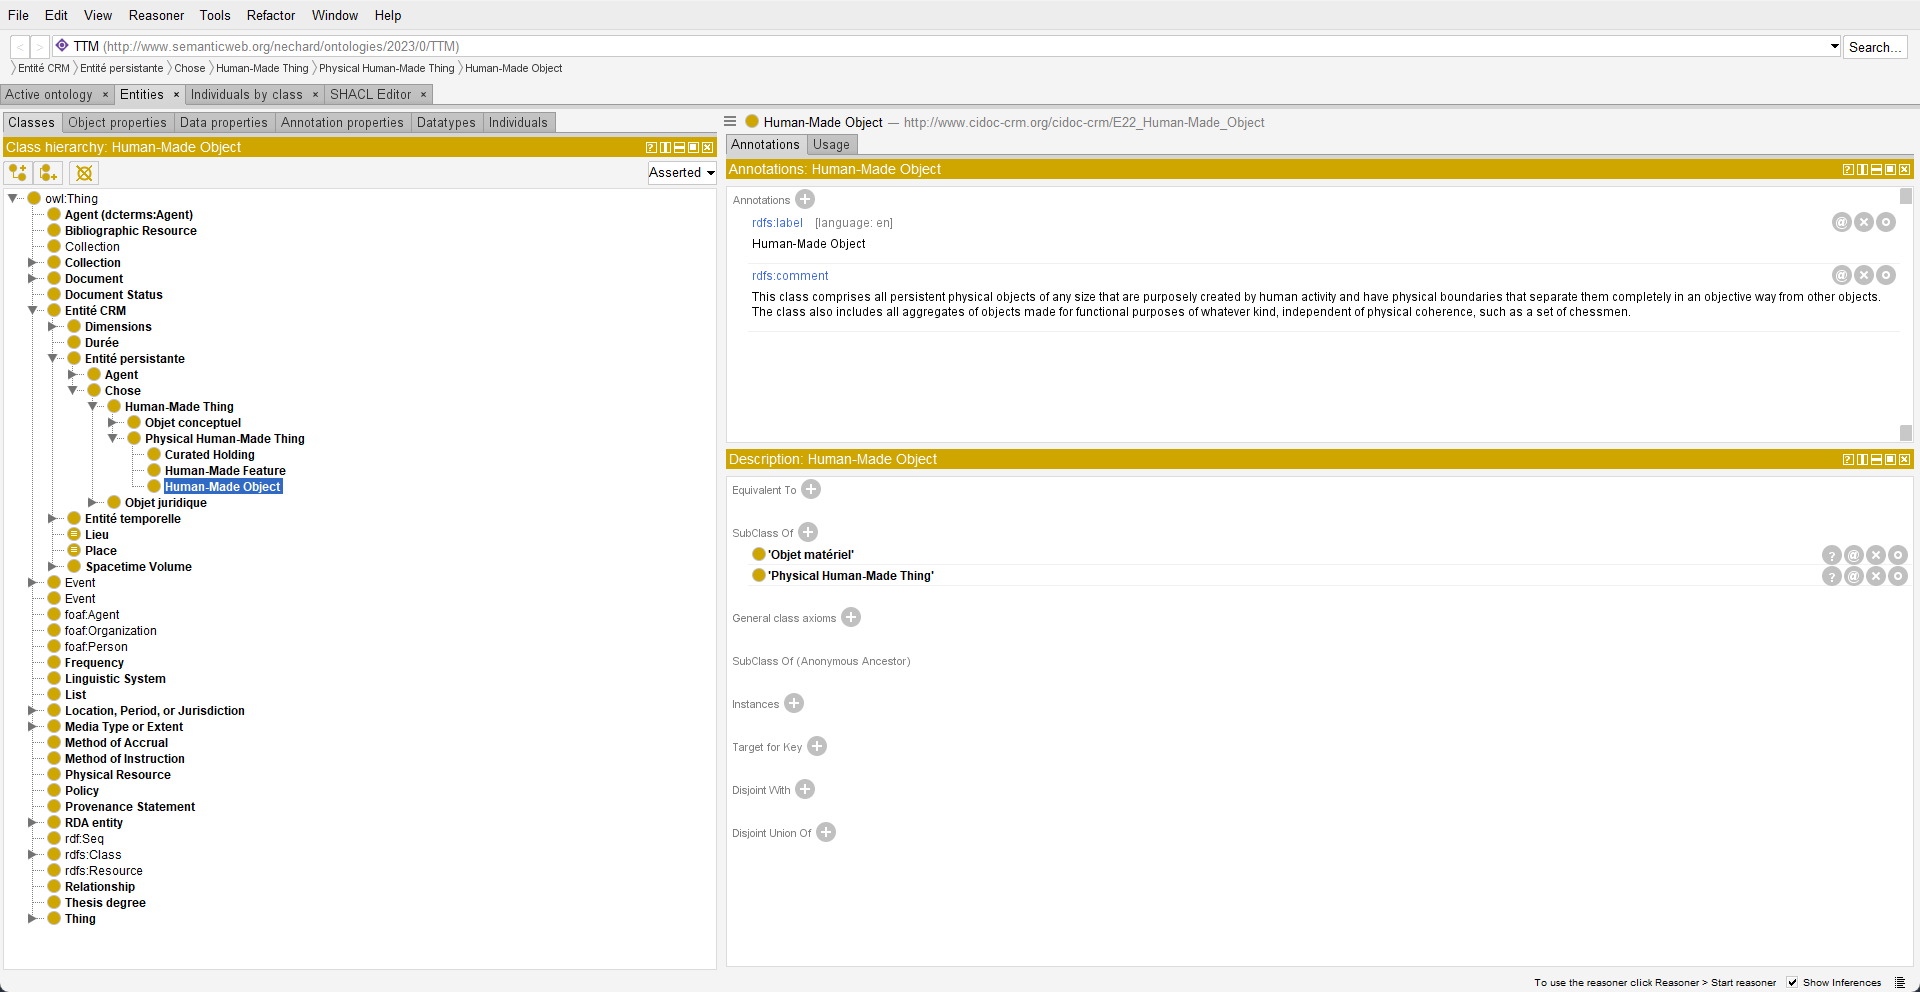
\includegraphics[width=1\textwidth]{assets/ontologie/Protege/screen_exemple_protege.png}
    \caption{Capture d'écran montrant l'interface de Protégé (visualisation de la classe \textbf{crm:E22 Human-Made Object})}
    \label{fig:screenExempleProtege}
\end{figure}

\subsubsection{Le cas spécial des flux}

\paragraph{} \hspace{10mm}
Une des difficultés auxquelles nous avons dû faire face avec Cyril et Matthieu est la modélisation des flux. De base \textbf{CIDOC-CRM} ne dispose pas de classe spécialement dédiée. Nous avons donc eu le choix entre deux options : trouver une nouvelle ontologie à intégrer à la nôtre ou bien tenter d'utiliser la classe \textbf{crm:E9 Move} du CIDOC-CRM malgré le nombre restreint de propriétés existantes dû au fait que CIDOC-CRM n'a pas été pensée pour ça. Pour des raisons de praticité (i.e. limiter au maximum le nombre d'ontologies que nous utilisons), nous avons opté pour la deuxième option. Au moment où nous avons fait ce choix, nous ne savions pas si il pourrait être concluant, Matthieu Quantin n'ayant jamais été confronté à cette situation auparavant.

\paragraph{} \hspace{10mm}
Pour pouvoir modéliser les flux de la manière la plus simple possible, nous avons scindé le problème en sous-problèmes : 
\begin{itemize}
    \item[\ding{103}] comment lier le flux à ce qui a été déplacé ?
    \item[\ding{103}] comment lier le flux à la durée du déplacement ?
    \item[\ding{103}] comment lier le flux au lieu de départ et au lieu d'arrivée ?
    \item[\ding{103}] comment faire si le flux peut (ou doit) être divisé en sous-flux ?
\end{itemize}

\paragraph{} \hspace{10mm}
Au final, nous avons réussi assez rapidement à résoudre ces sous-problèmes en fouillant dans la documentation. CIDOC-CRM possède précisément les bonnes propriétés dont nous avons eu besoin, et sont au nombre de 5 pour les plus utiles : 
\begin{itemize}
    \item[\ding{103}] \textbf{crm:P25 Moved} permet de modéliser ce qui a été déplacé. La range de la propriété est un \textbf{crm:P19 Physical Object}.
    \item[\ding{103}] \textbf{crm:P191 had duration} permet d'indiquer le temps de déplacement du point de vue quantitatif (valeur numérique) et dimensionnelle.
    \item[\ding{103}] \textbf{crm:P26 Moved to} et \textbf{crm:P27 Moved from} permettent de modéliser le point de départ et d'arrivée du flux. Ils doivent être des endroits physiques car la range de la propriété est \textbf{crm:P53 Place} (il faut donc utiliser d'autres propriétés pour un transfert d'argent d'un compte bancaire à un autre par exemple).
    \item[\ding{103}] \textbf{crm:P9 Consists of} permet de découper un flux en sous-flux. C'est donc une propriété symétrique dont le domaine et la range sont \textbf{crm:E9 Move}.
\end{itemize}

\begin{figure} [H]
    \centering
    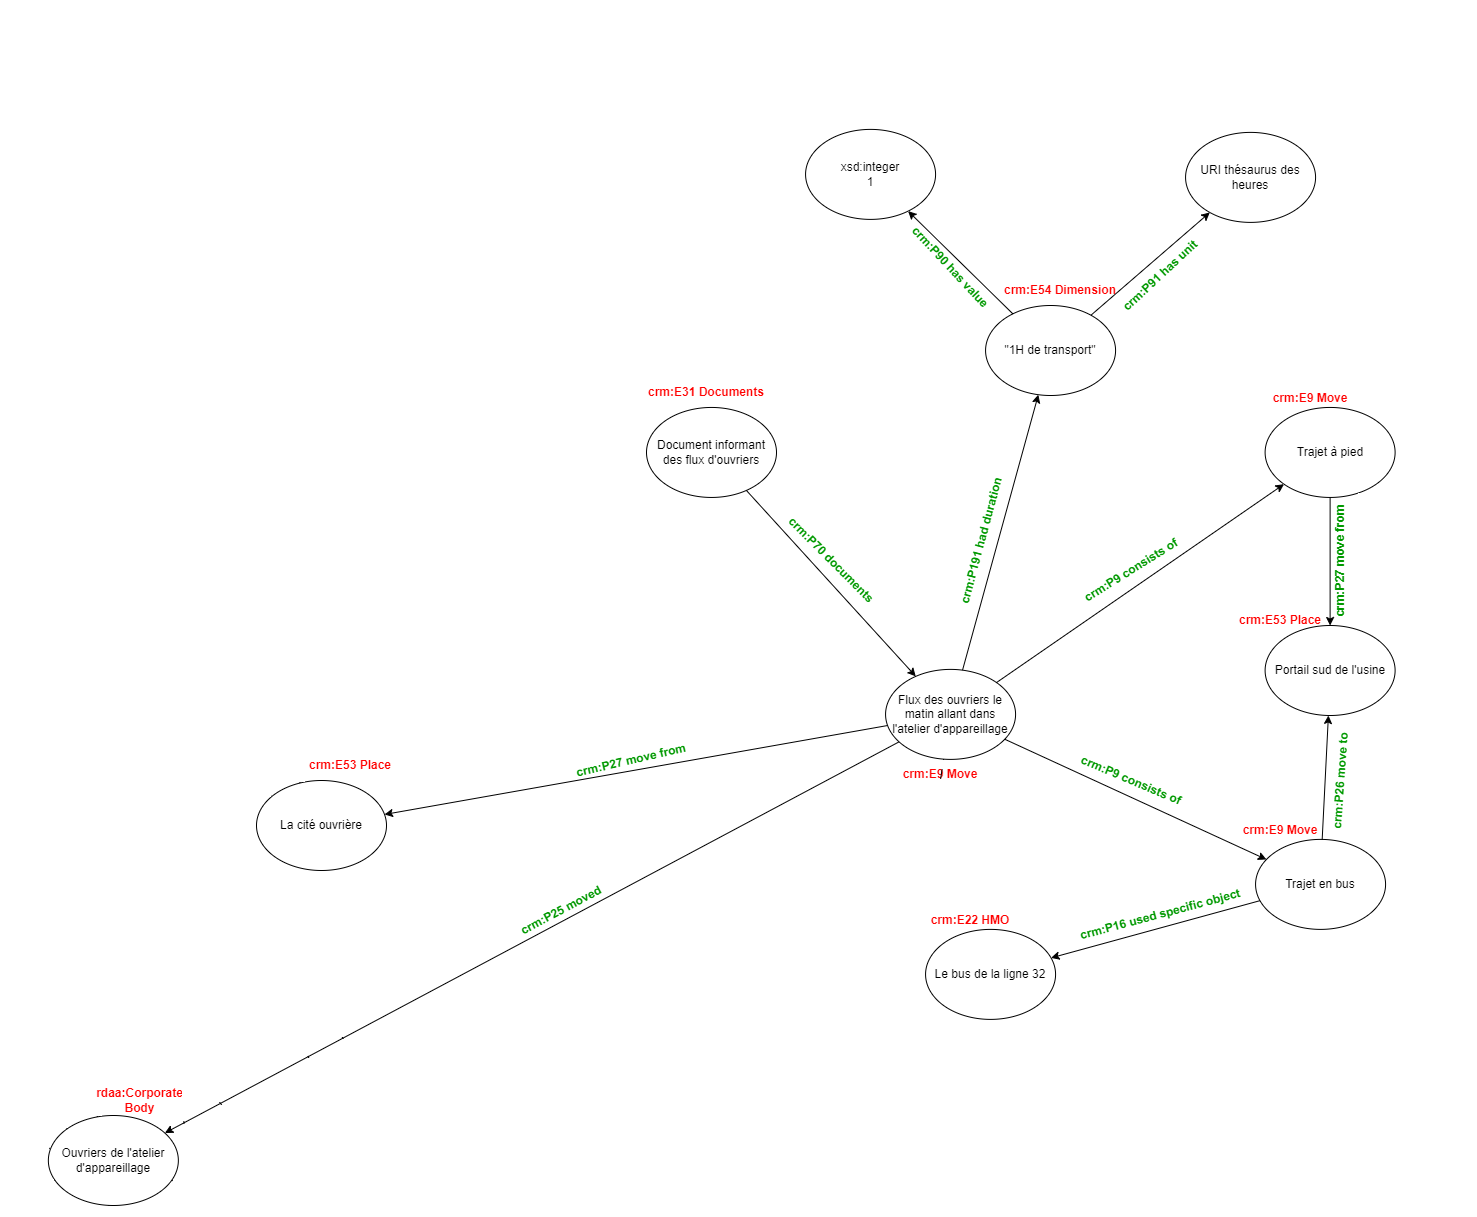
\includegraphics[width=1\textwidth]{assets/ontologie/screen_flux.png}
    \caption{Schéma montrant la modélisation des flux (extrait du schema général)}
    \label{fig:screenFlux}
\end{figure}

\subsection{Omeka-S et saisie des données}

\paragraph{} \hspace{10mm}
Pour créer la nouvelle base de données basée sur un modèle ontologique, deux choix ce sont présentés à nous : \textbf{Omeka-S} ou un système de \textbf{triple-store}. Malgré la capacité du triple-store à stocker une très grande quantité de données, nous avons choisi d'utiliser Omeka-S pour plusieurs raisons : 
\begin{itemize}
    \item[\ding{103}] tout d'abord, Omeka-S est bien plus simple à mettre en place et à utiliser qu'un triple-store.
    \item[\ding{103}] ensuite, le fait que l'ancienne base du projet ne contenait pas de données a beaucoup influencé notre choix. Si l'ancienne base avait déjà été remplie, il aurait fallu "transvaser" les données d'une base à l'autre ce qui aurait nécessité de créer un outil spécial pour convertir le format des données, d'autant plus  qu'il est beaucoup plus simple de transférer ces données vers un triple-store que vers Omeka-S. Par conséquent, dans le cas où l'ancienne base aurait été remplie, il aurait été pertinent d'utiliser un triple-store mais puisque ce n'est pas le cas, Omeka-S reste une bonne option.
    \item[\ding{103}] enfin, les compétences et connaissances de Matthieu Quantin sur Omeka-S, ainsi que le fait qu'il n'ait jamais mis en place de triple-store ont entériné notre choix.
\end{itemize}

\begin{figure} [H]
    \centering
    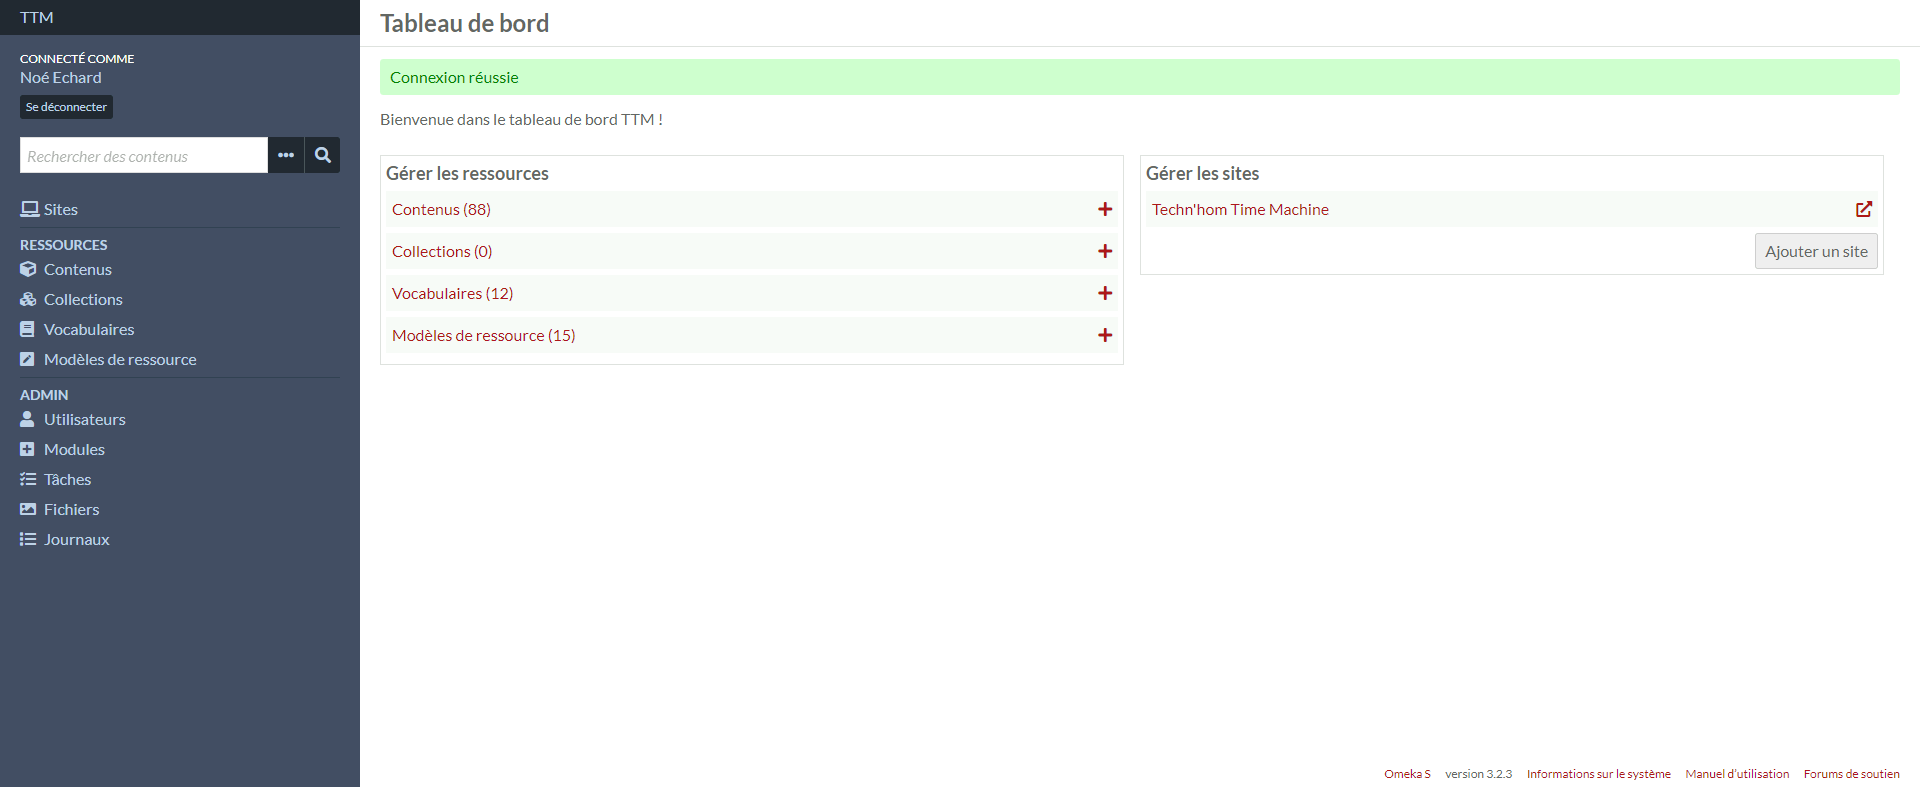
\includegraphics[width=1\textwidth]{assets/omeka/panneau_admin_omekapng.png}
    \caption{Écran d'accueil du panneau administrateur d'Omeka-S}
    \label{fig:panneauAdminOmeka}
\end{figure}

\subsubsection{Mise en place d'Omeka}

\paragraph{} \hspace{10mm}
L'un des principaux avantages d'Omeka-S est son aspect "clé en main". Malgré la rigidité qu'une telle caractéristique impose, Omeka-S reste assez ouvert au niveau de la personnalisation et du paramétrage. C'est donc la première tâche à laquelle nous nous sommes attelés avant de commencer à saisir les données. 

\paragraph{} \hspace{10mm}
Parmi tout ce que nous avons eu à faire, nous avons tout d'abord commencé par créer toutes les pages (autres que celle qui affiche les données) visibles sur le site web. Parmi ce qui avait été fait par Gabriel et Guillaume, nous avons repris les pages présentant le projet et l'équipe de travail et nous avons créé deux pages, nommées assez logiquement "Projet" et "Equipe" (voir Annexe 3, \hyperref[fig:pageProjetOmeka]{figure 3.16} et \hyperref[fig:pageEquipeOmeka]{figure 3.17}).

Ensuite, nous avons installé des thèmes et extensions. Parmi tous les thèmes disponibles, nous en avons pris quelques-uns qui nous semblaient convenir pour le projet afin de les tester. Au final, nous avons selectionné le thème "Center Row". Nous avons également installé des extensions, notamment celle nommé "Log" et qui permet d'avoir tous les logs des erreurs ou warnings directement dans le panneau d'admin via un onglet dédié.

\begin{figure} [H]
    \centering
    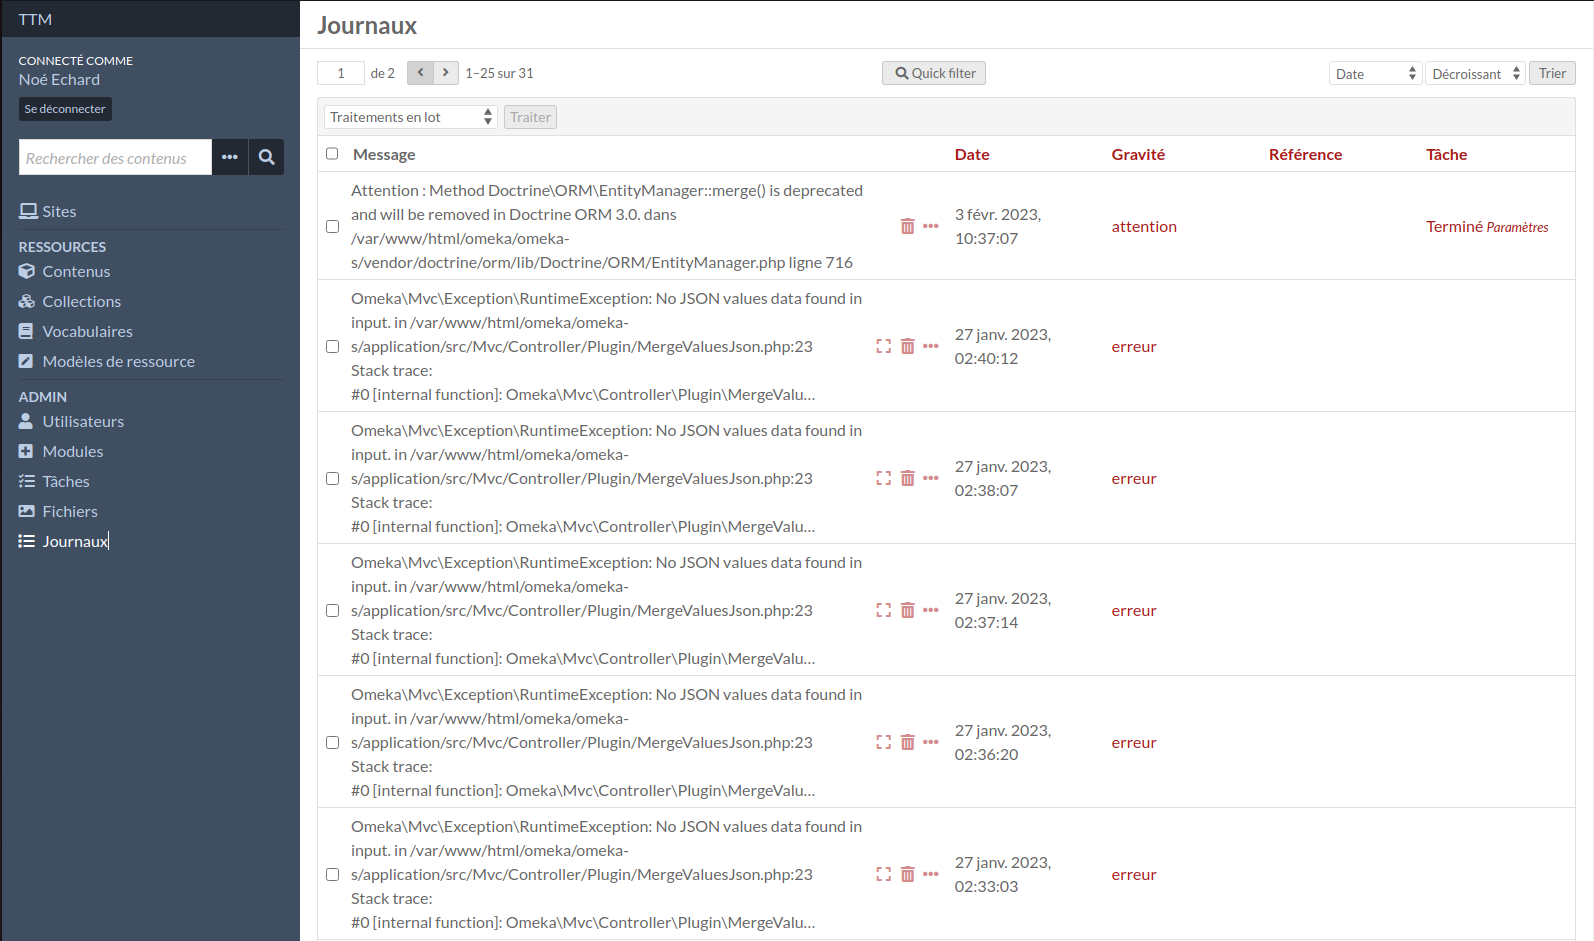
\includegraphics[width=1\textwidth]{assets/omeka/onglet_logs_omeka.png}
    \caption{Onglet des logs d'Omeka-S}
    \label{fig:ongletLogsOmeka}
\end{figure}

\subsubsection{Saisie des données}

\paragraph{} \hspace{10mm}
Une fois la "mise en place globale" terminée, nous nous sommes occupés de celle pour les ontologies et la saisie des données. La première étape a été de charger tous les vocabulaires\footnote{Comprendre ontologie} nécessaires à la saisies des données. Certains sont présents de base (comme \textbf{owl} ou \textbf{rdf} par exemple) mais la plupart doivent être chargés à l'aide du fichier contenant la déclaration de l'ontologie et du namespace\footnote{URL où se trouve le code de la déclaration sur internet}.

\begin{figure} [H]
    \centering
    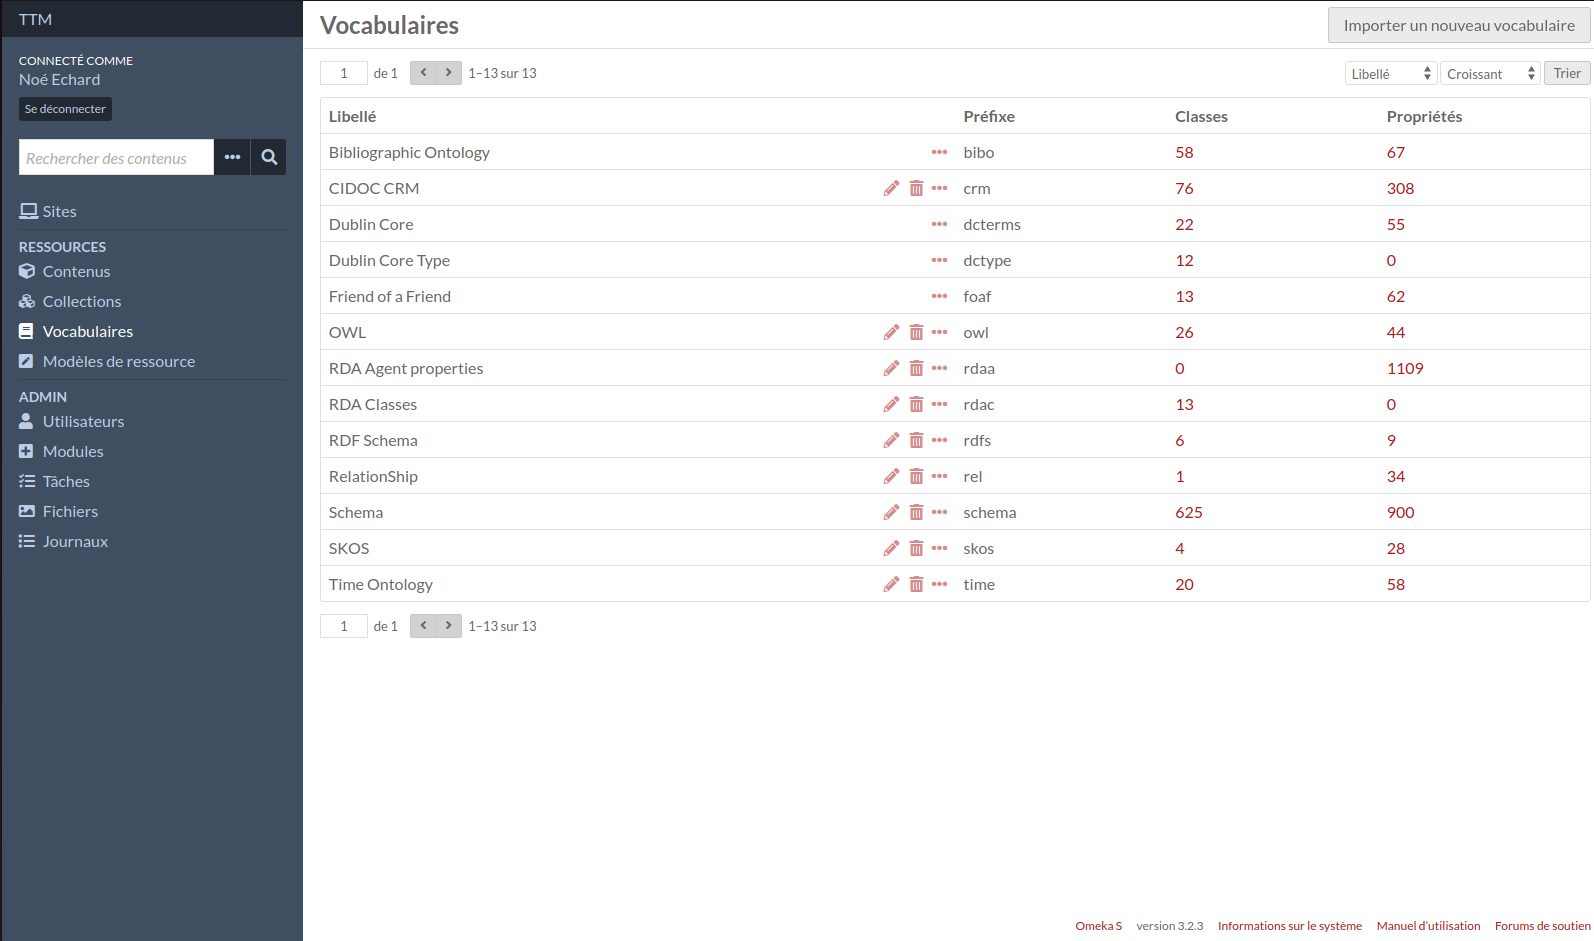
\includegraphics[width=0.82\textwidth]{assets/omeka/onglet_vocabs_omeka.png}
    \caption{Onglet des vocabulaires chargés dans Omeka-S}
    \label{fig:ongletVocabsOmeka}
\end{figure}

\paragraph{} \hspace{10mm}
Une fois les vocabulaires chargés, il ne manque plus qu'une étape avant de pouvoir saisir les données : créer des modèles de ressources. Même s'ils ne sont techniquement pas obligatoires, leur utilisation est presque requise tant le gain de temps est grand lorsque l'on enregistre des données. D'autant plus qu'ils permettent d'imposer certaines règles à ceux qui les utilisent.

De fait, tous les modèles de données que nous avons créés possèdent plusieurs caractéristiques :
\begin{itemize}
    \item[\ding{103}] La ressource créée a toujours un champ \textbf{skos:prefLabel} quelle que soit sa classe, et sa saisie est obligatoire.
    \item[\ding{103}] Le champ \textbf{skos:prefLabel} est affiché en tant que titre de ressource (par défaut le titre est de type \textbf{dcterms:title}).
    \item[\ding{103}] Toutes les propriétés ont un nom d'affichage renommé. Cela permet d'avoir un nom français, propre et lisible sur le site (par exemple, "hasDateOfBirth" devient "Date de naissance"). De surcroît, toutes les propriétés utilisées pour enregistrer un item qui ne sont pas dans le modèle de ressource ne peuvent pas être renommées pour l'affichage du site.
\end{itemize}

\begin{figure} [H]
    \centering
    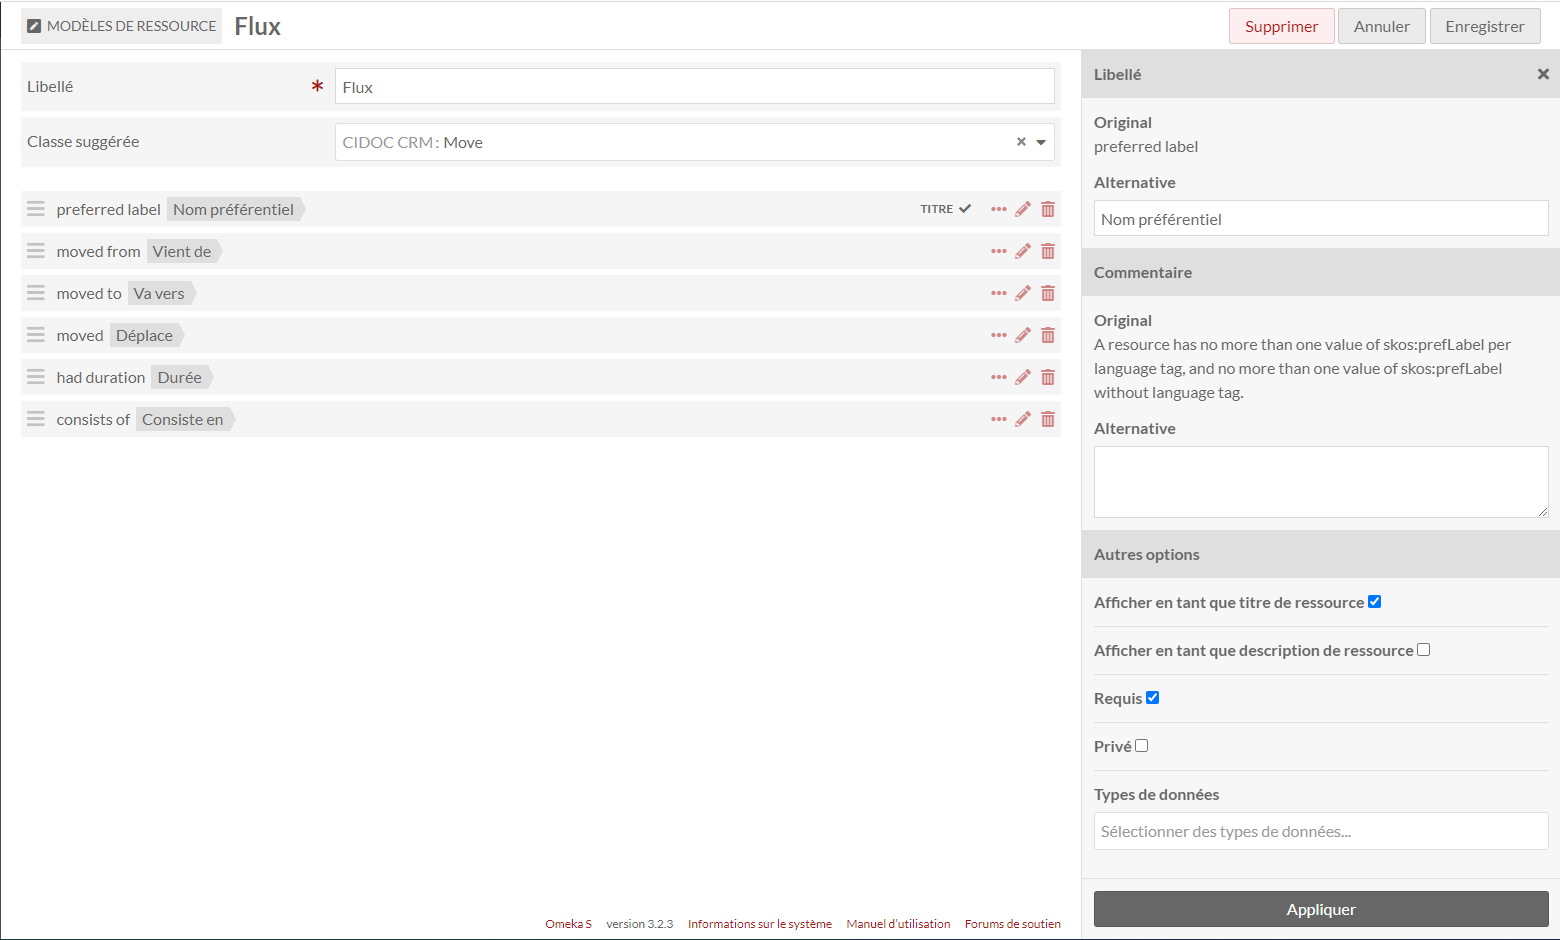
\includegraphics[width=1\textwidth]{assets/omeka/screen_omeka_modele_ressource.png}
    \caption{Exemple de modèle de ressource en cours d'édition}
    \label{fig:modeleRessourceOmeka}
\end{figure}

\paragraph{} \hspace{10mm}
Après avoir terminé la préparation, nous avons enfin pu commencer à saisir des données. Les premiers items que nous avons documentés sont tous tirés du manuel Roret intitulé "Nouveau manuel complet du filateur". Cyril s'est chargé de son analyse, puis a synthétisé toutes les informations utiles dans un document Word à l'aide de tableaux et de petits textes explicatifs. A partir de son document d'analyse, nous avons pu dresser dans un premier temps le schéma décrivant la production de coton (\hyperref[fig:schemaRoretTTM]{figure 3.17}), et c'est seulement dans un second temps que nous avons saisi les données.

\begin{figure} [H]
    \centering
    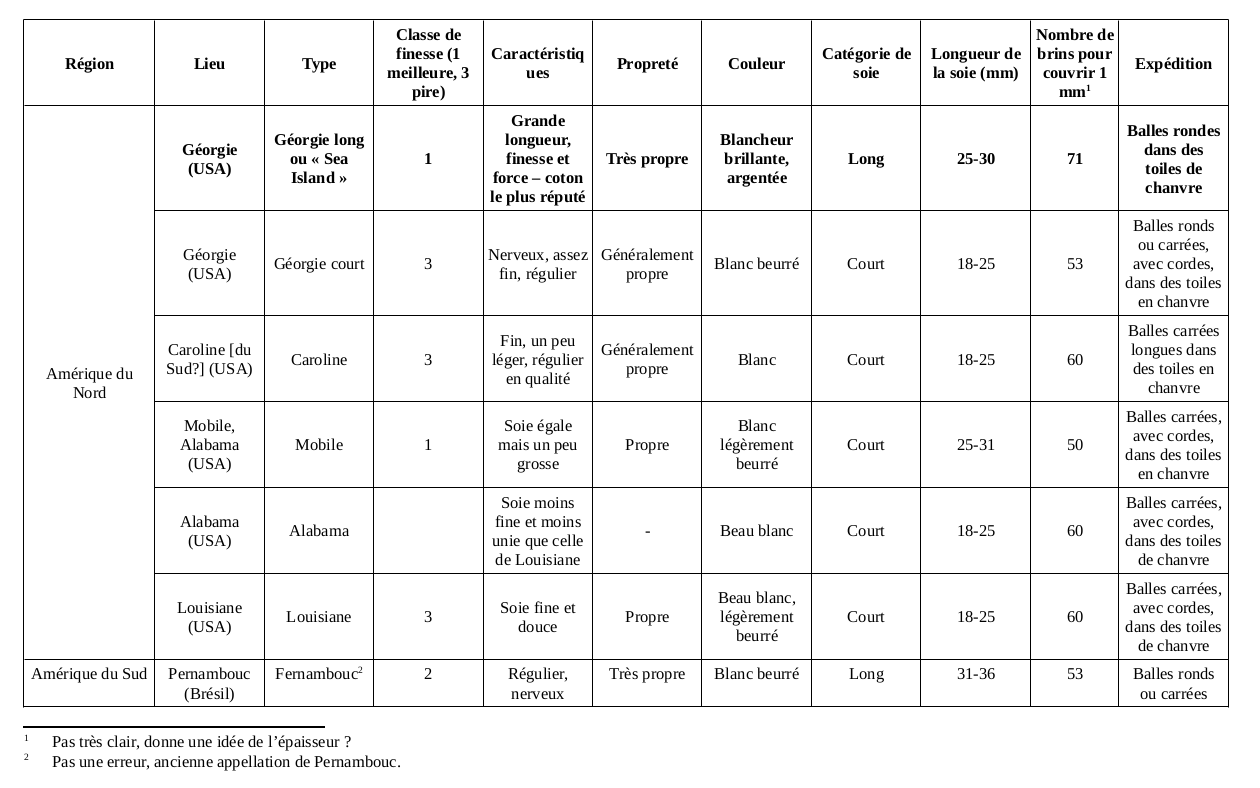
\includegraphics[width=1\textwidth]{assets/divers/screen_cotons.png}
    \caption{Exemple de tableau récapitulant les informations à enregistrer pour certains types de cotons}
    \label{fig:screenTableauCoton}
\end{figure}

\subsection{Thésaurus}

\paragraph{} \hspace{10mm}
L'un des aspects essentiels de l'utilisation d'ontologies sont les thésaurus documentaires. Ils permettent de lier des items non normalisés et non contrôlés à des listes de termes qui eux, le sont. L'utilisation de thésaurus est primordiale, car elle permet de faciliter les alignements entre différentes ontologies, fondement essentiel à leur existence même.

Dans le cadre de notre projet, et dans la volonté de suivre les normes de l'industrie, nous avons utilisé les ontologies suivantes :
\begin{itemize}
    \item[\ding{103}] \href{https://viaf.org/}{VIAF}, pour les personnes (ne fonctionne que si elles sont connues).
    \item[\ding{103}] \href{https://sws.geonames.org/}{GeoNames}\footnote{attention, l'URL est sws.geonames.org et non pas www.geonames.org}, pour les lieux
    \item[\ding{103}] \href{https://www.getty.edu/research/tools/vocabularies/aat}{Art and Architecture Thésaurus du Getty Museum}, pour toute notion autre qu'une personne ou un lieu
    \item[\ding{103}] \href{http://data.culture.fr/thesaurus/}{Les vocabulaires du Ministère de la Culture et de la Communication}, ici aussi pour toute notion autre qu'une personne ou un lieu (à la condition bien sûr, que le thésaurus détienne cette notion)
\end{itemize}

\paragraph{} \hspace{10mm}
Pour qu'un item soit lié à un thésaurus, nous devons utiliser la propriété \textbf{owl:sameAs}. De plus, bien que ces thésaurus possèdent l'essentiel des notions dont nous pourrions avoir besoin, nous avons aussi à disposition l'Opentheso\footnote{Opentheso est un logiciel de stockage de thésaurus en ligne} du projet "Huma-Num". Celui-ci regroupe toutes sortes de thésaurus portant sur des notions de Sciences Humaines et Sociales, le patrimoine industriel étant l'une d'entre elles. De plus, il regroupe tous les vocabulaires du Ministère de la Culture (nommé ci-avant) et permet de les parcourir via un arbre conceptuel, ce qui est plus rapide que de parcourir une par une les pages du site du ministère (sans parler du fait que le site du ministère est terriblement lent).  

\begin{figure} [H]
    \centering
    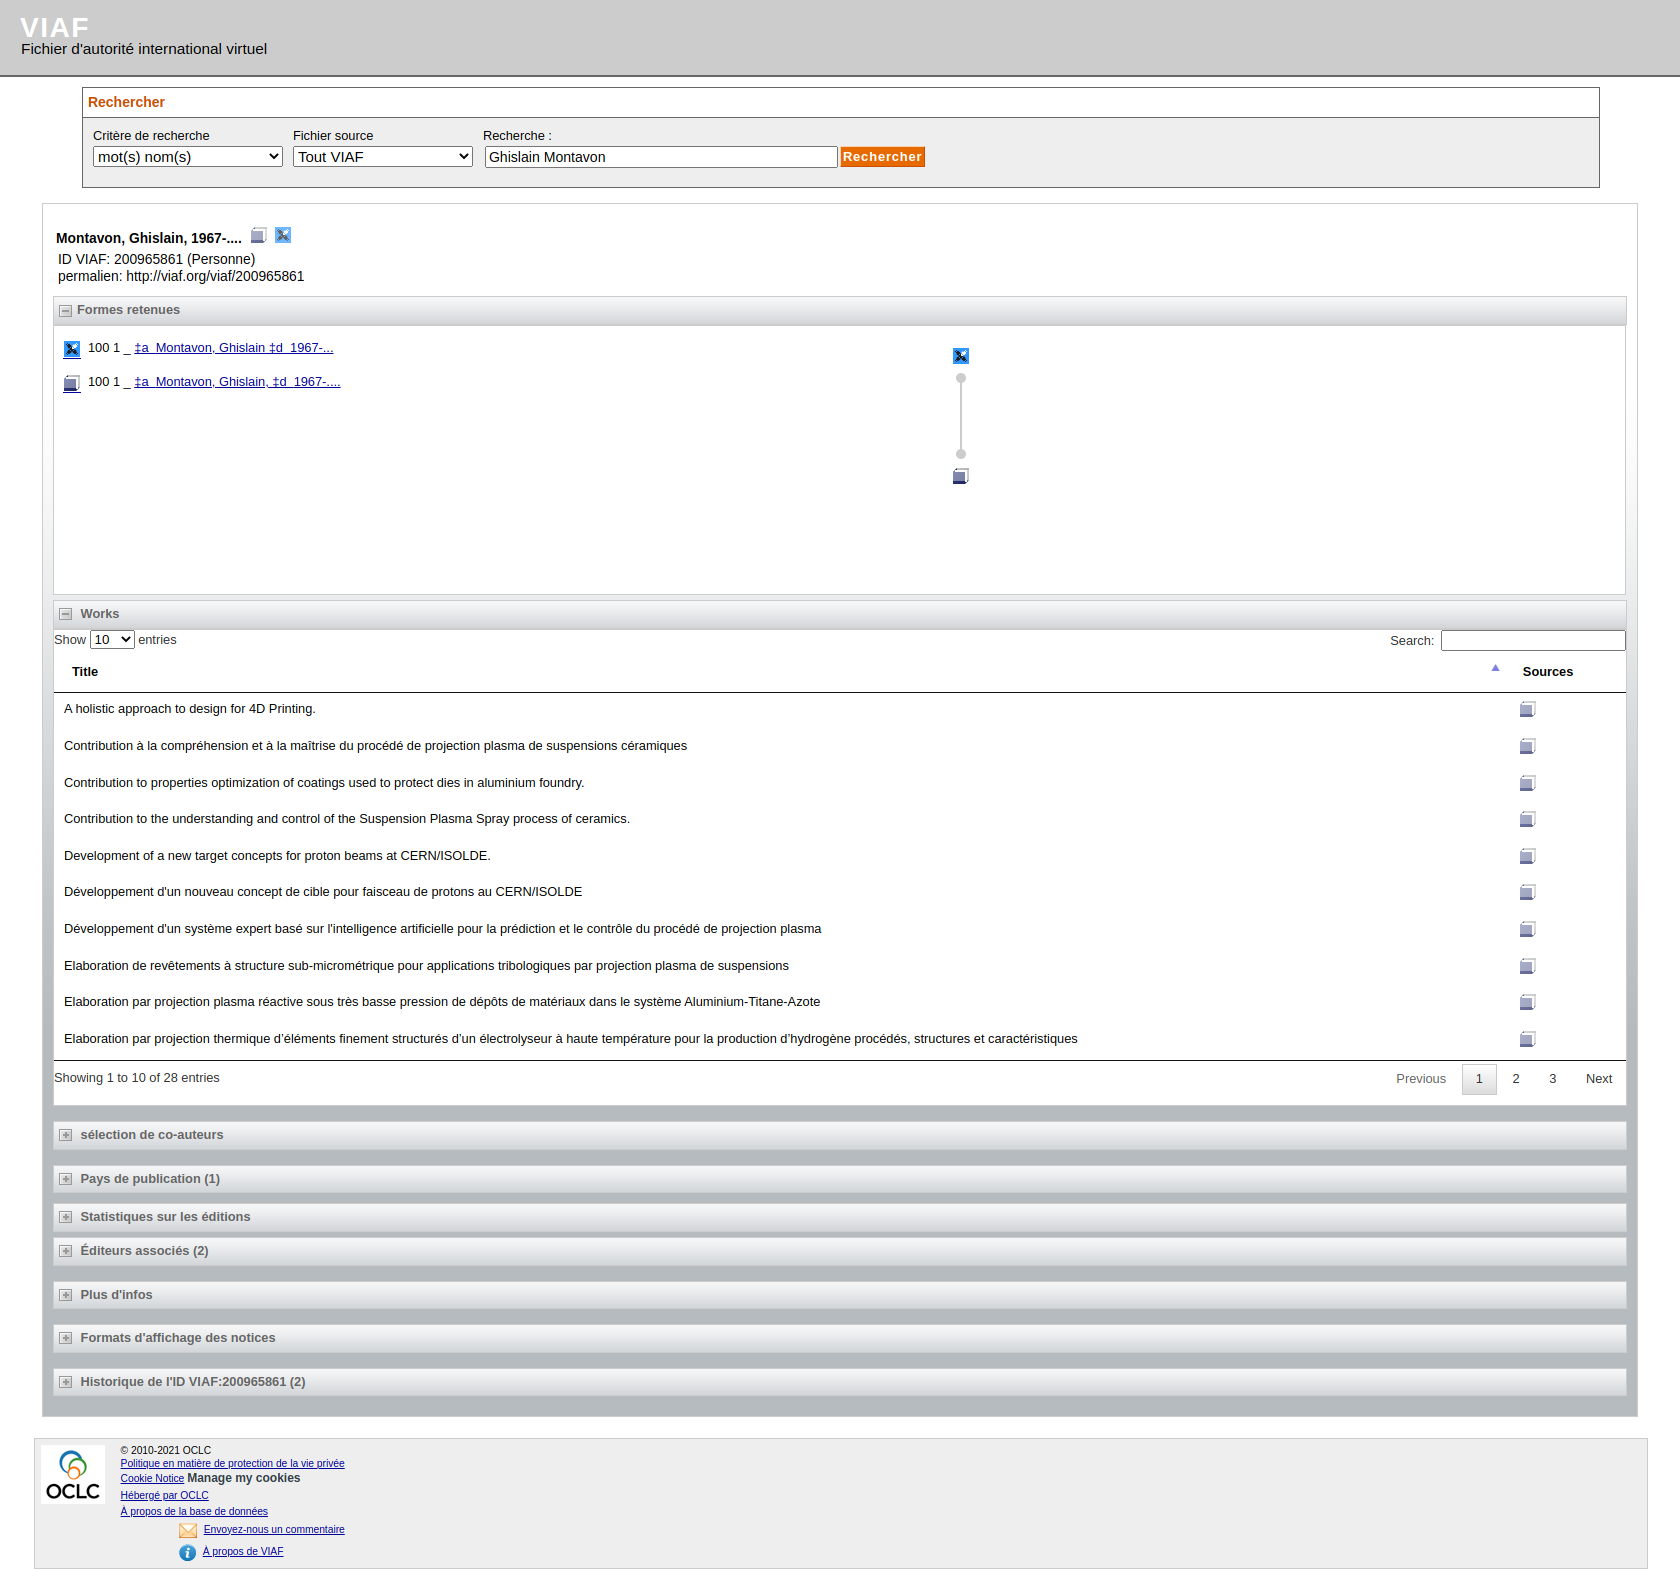
\includegraphics[width=1\textwidth]{assets/thesaurus/screen_viaf_ghis.png}
    \caption{Fiche VIAF de M. Ghislain Montavon}
    \label{fig:viafGhis}
\end{figure}

\subsection{Validation et SHACL}

\paragraph{} \hspace{10mm}
Avant que tout ce qui concerne la déclaration de notre ontologie et la saisie des données ne soit réellement terminé, il reste une étape cruciale à réaliser : la validation via la spécification SHACL (Shapes Constraints Language). Cette validation a deux intérêts majeurs :
\begin{itemize}
    \item[\ding{103}] s'assurer que les données saisies respectent bien les règles de notre ontologie (donc cela permet de corriger les erreurs).
    \item[\ding{103}] vérifier que notre ontologie en elle-même ne brise pas de règles logiques ou qu'il n'y ait pas d'incohérences.
\end{itemize}

\vspace{10mm}
Pour pouvoir mettre en place la validation, nous nous sommes aidés de deux outils :
\begin{itemize}
    \item[\ding{103}] Protégé et son plugin \textbf{SHACL4Protégé}
    \item[\ding{103}] l'outil de conversion de SPARNA : \hyperlink{https://shacl-play.sparna.fr/play/convert}{SHACL Play ! Convert}
\end{itemize}

\paragraph{} \hspace{10mm}
Ces deux outils ne peuvent fonctionner l'un sans l'autre : tout d'abord, à l'aide de "SPARNA Play !" et de notre fichier contenant notre ontologie, on génère un fichier SHACL qui va nous permettre de tester la validité de notre travail. Ensuite, à l'aide de Protégé, on charge le fichier SHACL puis on l'applique sur le fichier OWL contenant nos triplets de données. En sortie nous obtenons les erreurs si il y en a, leur type et leur triplet d'origine. Toutefois, avant d'appliquer le fichier SHACL sur nos triplets, il faut mettre en route le raisonneur de Protégé. Son rôle est de vérifier si il n'y a pas d'incohérence du point de vue de la logique pure (comme par exemple un objet qui a pour types deux classes qui sont déclarées comme ne pouvant pas partager d'instances communes). Si le raisonneur détecte des irrégularités, il nous en informe via un onglet de logs en nous précisant d'où viennent les erreurs (de la même manière qu'un compilateur classique) et nous devons les corriger avant de pouvoir passer à la validation via SHACL.

\pagebreak
\section{Unity 3D : Modélisation des flux}

\paragraph{} \hspace{10mm}
La dernière partie de mon travail sur ce projet porte sur Unity. A terme, un des objectifs du projet Techn'hom Time Machine est d'avoir une application en Réalité Virtuelle permettant de se déplacer dans le Techn'hom. Il semble évident qu'avec le travail que j'ai déjà accompli et la durée de mon stage, je ne suis pas en mesure de pouvoir développer une telle application. C'est pourquoi dans un premier temps, il a été décidé de créer une application en 3D permettant de visualiser les flux que les données saisies nous ont renseignés. Ici aussi, le manque de temps et mon inexpérience sur Unity font que je ne suis pas en mesure de faire une application complète avec une interface permettant de choisir quel flux afficher. Nous avons donc choisi de faire une maquette de cette application qui permettrait de visionner un seul flux.

\subsection{Schématisation de l'usine}

\paragraph{} \hspace{10mm}
La première partie de notre travail a été la modélisation en 3D du Techn'nom, et plus précisément de l'ancienne usine DMC. Le plus important était d'avoir une carte et des bâtiments parfaitement à l'échelle pour plus de réalisme. Pour ce faire, nous nous sommes appuyés sur un plan de l'usine que Cyril nous a fourni et datant de 1930.

\begin{figure} [H]
    \centering
    \includegraphics[width=1\textwidth]{assets/unity/schema_usine_dmc.jpg}
    \caption{Plan de l'usine DMC}
    \label{fig:planDMC}
\end{figure}

\paragraph{} \hspace{10mm}
Une fois le plan à disposition, nous en avons conclu que la manière la plus simple de modéliser les différents bâtiments à la bonne échelle était simplement de créer un sol dans Unity qui aurait pour texture l'image du plan. Les deux seuls points que nous avons eu à vérifier étaient que l'image ne perde pas ni en qualité ni en résolution lorsqu'on l'appliquerait sur la texture du sol et qu'elle ne se déformerait pas sinon quoi tout ceci n'aurait aucun intérêt.

Par la suite, comme l'application n'en est encore qu'au stade de maquette, nous nous sommes contentés de représenter les bâtiments par de simples rectangles blancs, numérotés selon les indications du plan. Ceux ci sont simplement des objets du type primitif \textbf{Cube} intégré à Unity que l'on a positionnés et dimensionnés par tâtonnement par dessus le plan.

\begin{figure} [H]
    \centering
    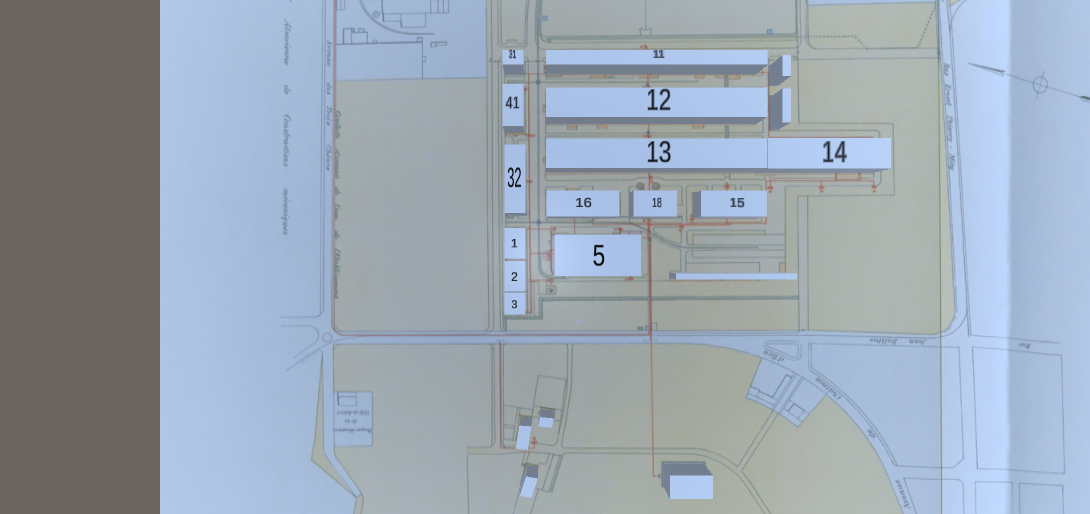
\includegraphics[width=0.79\textwidth]{assets/unity/screen_unity_map.png}
    \caption{Carte de l'application Unity vue du dessus}
    \label{fig:unityMap}
\end{figure}

\subsection{Génération procédurale des flèches}

\paragraph{} \hspace{10mm}
La deuxième partie de notre travail a été de trouver un moyen de faire afficher à l'écran des flèches. Par défaut, Unity ne possède pas ce genre d'objet en type primitif (comme les \textbf{Cube}), il a donc fallu trouver un moyen d'en disposer. La première chose à laquelle nous avons pensé est de trouver un asset sur l'Unity Asset Store. Malheureusement, il n'existe aucun asset gratuit sur le store qui puisse répondre à nos besoins ; seuls certains assets payants étaient intéressants. La deuxième option à laquelle nous avons pensé est le design d'un asset sur Blender. Toutefois, cette option a très vite été écartée car je n'ai aucune connaissance sur Blender, et nous avons donc préféré chercher une autre solution. Enfin, la troisième option à laquelle nous avons réfléchi et que nous avons choisi, est la génération procédurale. La génération procédurale a l'avantage d'être plutôt simple à mettre en oeuvre, et surtout, d'être plus personnalisable qu'un asset pré-fait venant du store.

\begin{figure} [H]
    \centering
    
\includegraphics[width=0.5\textwidth]{assets/unity/screen_fleche2.png}
    \caption{Dessin montrant la flèche générée}
    \label{fig:dessinFleche2}
\end{figure}

\paragraph{} \hspace{10mm}
Pour pouvoir modéliser des flèches, nous avons choisi d'utiliser les \textbf{Mesh} intégrés à Unity. La première étape a été la modélisation de la "queue" : nous avons commencé par générer quatre points pour former un rectangle en partant de l'origine du Mesh, puis nous avons formé deux triangles rectangles dont les hypoténuses se superposent pour former un rectangle. Le positionnement des points dépend de 2 paramètres, ce qui permet de régler la largeur et la longueur de la queue. 

\begin{figure}[H]

\centering

\begin{subfigure}{0.49\textwidth}
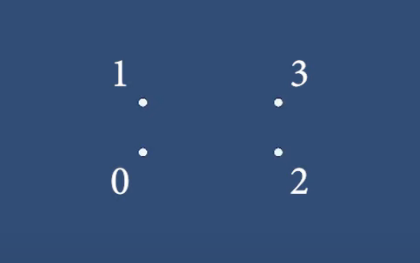
\includegraphics[width=1\linewidth]{assets/unity/screen_point1.png} 
\label{fig:unityPoint1}
\end{subfigure}
\begin{subfigure}{0.49\textwidth}
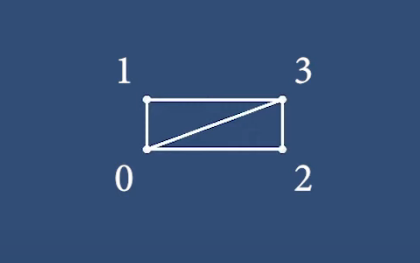
\includegraphics[width=1\linewidth]{assets/unity/screen_point3.png}
\label{fig:unityPoint3}
\end{subfigure}

\caption{Dessins montrant comment est générée la queue de la flèche}
\label{fig:unityPoint1&3}
\end{figure}

\paragraph{} \hspace{10mm}
Enfin, la deuxième partie du travail a été la modélisation de la tête de la flèche. Pour ce faire, nous avons utilisé la même méthode que pour la queue mais en ne plaçant que 3 points pour former un triangle. Ces 3 points sont placés en bout de queue et dépendent eux aussi de deux paramètres afin de pouvoir changer la longueur et la largeur de la tête de la flèche.

\begin{figure}[H]

\centering

\begin{subfigure}{0.49\textwidth}
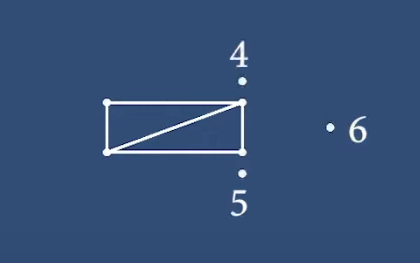
\includegraphics[width=1\linewidth]{assets/unity/screen_point2.png} 
\label{fig:unityPoint2}
\end{subfigure}
\begin{subfigure}{0.49\textwidth}

\includegraphics[width=1\linewidth]{assets/unity/screen_fleche1.png}
\label{fig:dessinFleche1}
\end{subfigure}

\caption{Dessins montrant comment est générée la tête de la flèche}
\label{fig:unityPoint2&Fleche1}
\end{figure}

\subsection{API Omeka-S et Représentation des flux}

\paragraph{} \hspace{10mm}
Après avoir fini de préparer tout ce qui concerne la partie graphique, nous avons commencé à travailler avec l'API d'Omeka-S. Cette dernière est plutôt simple à utiliser car elle n'est pas très complexe et surtout très bien documentée\footnote{Lien vers la documentation : \hyperlink{https://omeka.org/s/docs/developer/}{https://omeka.org/s/docs/developer/}}. 

\paragraph{} \hspace{10mm}
Pour pouvoir avoir des données exploitables, la première étape a été de dé-sérialiser les données au format JSON venant de l'API. Cette étape nous a posé quelques problèmes car la structure JSON des items d'Omeka est très irrégulière (les données sont toutes dans un tableau JSON dont les index ont des structures différentes), et dé-sérialiser à la main devient impossible dès lors que l'on a ne serait-ce que quelques items à gérer. Afin de ne pas rester bloqués, nous nous sommes tournés vers Anne Wartelle que nous avions rencontrée à Nantes et qui avait déjà travaillé avec une combinaison d'ontologie et d'Unity. Cette dernière nous a ainsi proposé d'utiliser \hyperlink{https://quicktype.io/}{Quicktype.io} : le site permet d'obtenir du code dé-sérialisant des données au format JSON dans le langage que l'on souhaite. Nous avons donc copié toutes les données de l'API directement depuis le navigateur et nous avons tout collé dans Quicktype. Le principal avantage de cette méthode est sa rapidité : en seulement 1 minute, nous avons eu à disposition du code tout prêt et parfaitement fonctionnel pour tout dé-sérialiser. En revanche, cette méthode comporte aussi un inconvénient : à chaque ajout d'item dans Omeka, notre script Unity devient incapable de gérer les données et nous sommes obligés de re-générer le code pour remplacer l'ancien.

\paragraph{} \hspace{10mm}
Ensuite, la deuxième étape a été de réfléchir à comment traiter les données et comment les exploiter pour pouvoir faire afficher les flux. Ici aussi, nous avons rencontré des problèmes pour trouver une solution durable, maintenable et extensible à cause de la variabilité de la structure des données.

Comme l'application en est encore au stade de maquette et que nous avons décidé de ne modéliser qu'un seul flux, cela simplifie un petit peu les choses : nous n'avons pas besoin de multiplier les requêtes vers le serveur pour obtenir les données voulues à chaque changement de flux à visualiser et l'exploitation est plutôt rapide. La première action à réaliser est d'isoler le flux que nous voulons afficher : pour cela, chaque classe d'objet est identifiée par un entier unique. Dans notre cas, les objets de type \textbf{crm:E9 Move} ont pour ID 114. Cet ID est très pratique car il peut être utilisé dans une query string en paramètre de l'URL pour effectuer des requêtes plus précises\footnote{La query string est : resource\_class\_id}.Une fois notre flux isolé, deux possibilités s'offrent à nous : soit le flux est composé de sous-flux, soit c'est un flux simple. Dans le cas d'un flux simple, il suffit de regarder quels sont le lieu de départ et le lieu d'arrivée du flux. Dans le cas du flux composé, il faut traiter chaque sous-flux un par en suivant le même procédé que pour les flux simples.

Enfin, une fois que nous avons su comment exploiter les données, nous avons réfléchi à comment gérer l'affichage. La solution que nous avons retenu est la suivante : nous pré-disposons des flèches qui vont de bâtiments en bâtiments (pour tous et dans les deux sens) que nous désactivons par défaut. Ensuite, à l'aide des données que l'on vient d'analyser, on détermine à l'aide de booléens quels sont les points de départs et d'arrivées\footnote{Les deux propriétés situant le flux étant distinctes, on connaît la cardinalité d'un flux}. Enfin, selon les booléens qui ont pour valeur \textbf{true}, on peut réactiver les flèches dont on a besoin.

\begin{figure} [H]
    \centering
    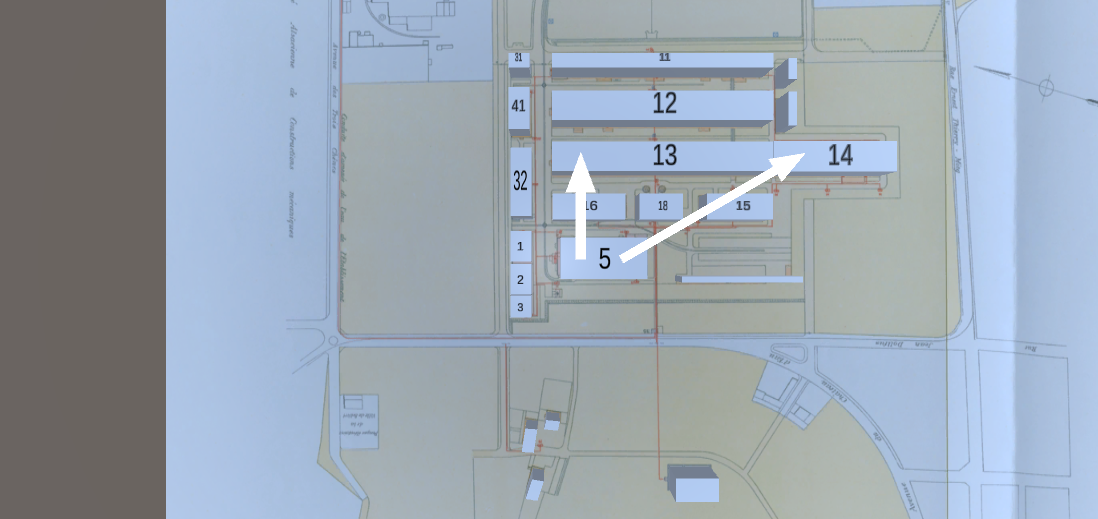
\includegraphics[width=1\textwidth]{assets/unity/screen_unity_flux.png}
    \caption{Modélisation d'un flux vu du dessus}
    \label{fig:unityFlux}
\end{figure}

% Expliquer comment on modélise les flux

    \chapter*{Conclusion}
\addcontentsline{toc}{chapter}{Conclusion}

\section*{Bilan du travail}
Dans l'ensemble, tous mes objectifs de travail ont été réalisés. Évidemment, tout n'est pas achevé (c'est même l'inverse, rien n'est terminé) mais au vu de l'évolution du projet, ce n'était pas le but de ma présence. Beaucoup de labeur reste à fournir que cela soit pour la formalisation de l'ontologie du projet que pour l'application Unity, tous deux étant encore à leurs débuts.

\vspace{5mm}
Je suis satisfait des résultats que j'ai obtenu ; même si mon travail n'est pas parfait, j'ai tout mis en oeuvre pour faire du mieux que j'ai pu, et je pense que mes efforts ont payé.

\section*{Bilan personnel}

Ce stage a été pour moi une grande satisfaction sur tous les plans.

Sur le plan personnel, j'ai découvert un pan de l'histoire de France que je ne connaissais très peu voire pas du tout. J'ai également pu faire la rencontre de personnes passionnées dans ce domaine et qui m'ont encore plus donné l'envie d'accroître ma culture générale et historique.

Sur le plan technique, j'ai découvert des technologies dont je ne connaissais même pas l'existence. Le concept d'ontologie a beaucoup changé ma vision de la science de l'information : la volonté de lier et structurer les données présentes sur internet est quelque chose qui m'avait déjà interpellé avant d'effectuer mon stage, mais seule la solution apportée à cette problématique m'échappait encore. J'ai également progressé dans les technologies Web en explorant les framework Django et Angular que je n'avais jamais utilisés, ainsi que dans le développement d'applications Unity que j'ai pu brièvement utiliser vers la fin du stage.

Enfin, j'ai pu accroître ma capacité à travailler en autonomie et ma persévérance dans le travail. Manipuler des logiciels et technologies encore peu exploités implique une absence d'aide conséquente sur internet, et je n'ai pu compter que sur la documentation et quelques personnes qualifiées pour outrepasser mes difficultés.

En conclusion, j'aimerais remercier encore une fois toutes les personnes que j'ai pu citer dans ce rapport ainsi que l'UTBM pour cette opportunité qui m'a été offerte et que je ne regrette pas d'avoir saisie.
    
    \nocite{*}
    \printbibliography
    \chapter*{Annexes}
\addcontentsline{toc}{chapter}{Annexes}

\section*{1. Schémas d'utilisation de l'ontologie}\label{annexe1}
\addcontentsline{toc}{section}{Schéma de base d'utilisation de l'ontologie}
\begin{figure} [H]
    \centering
    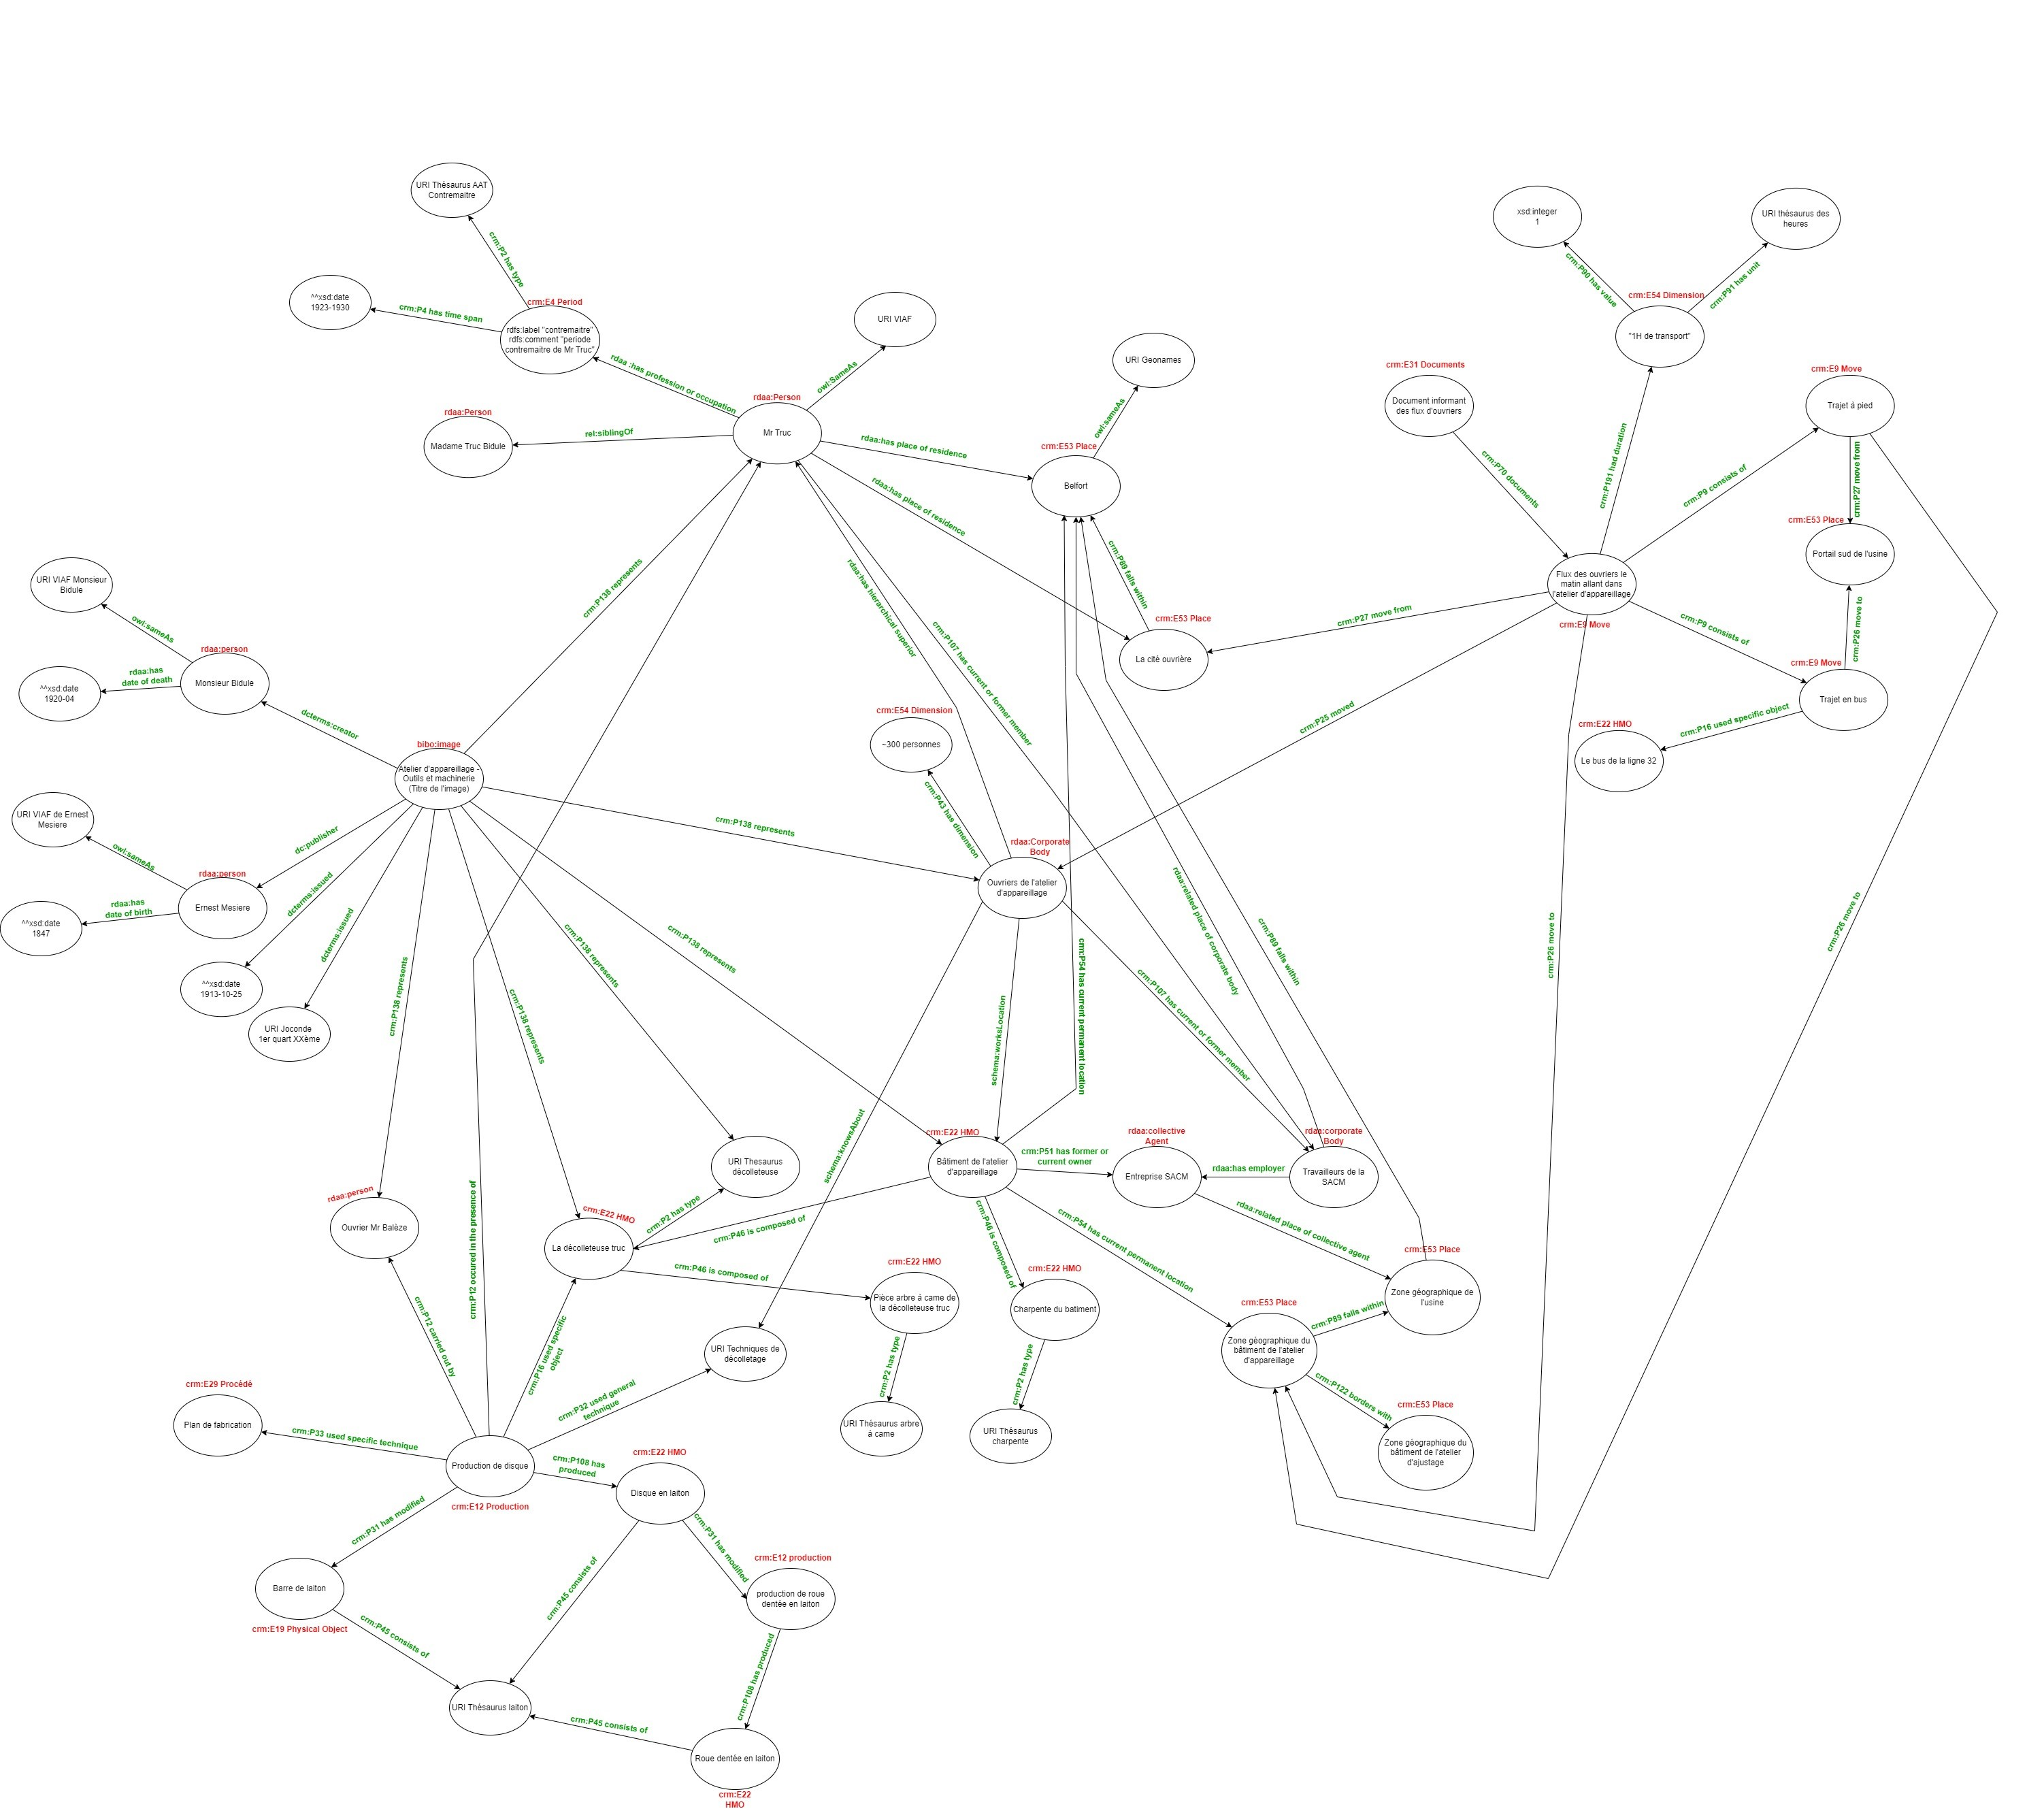
\includegraphics[width=1\textwidth]{assets/annexes/schema_base_ontologie_TTM.jpg}
    \caption{Schéma de base décrivant l'utilisation de l'ontologie dédiée au projet}
    \label{fig:schemaBaseTTM}
\end{figure}

\addcontentsline{toc}{section}{Schéma décrivant la production de fil de coton à l'aide du Manuel Roret}
\begin{figure} [H]
    \centering
    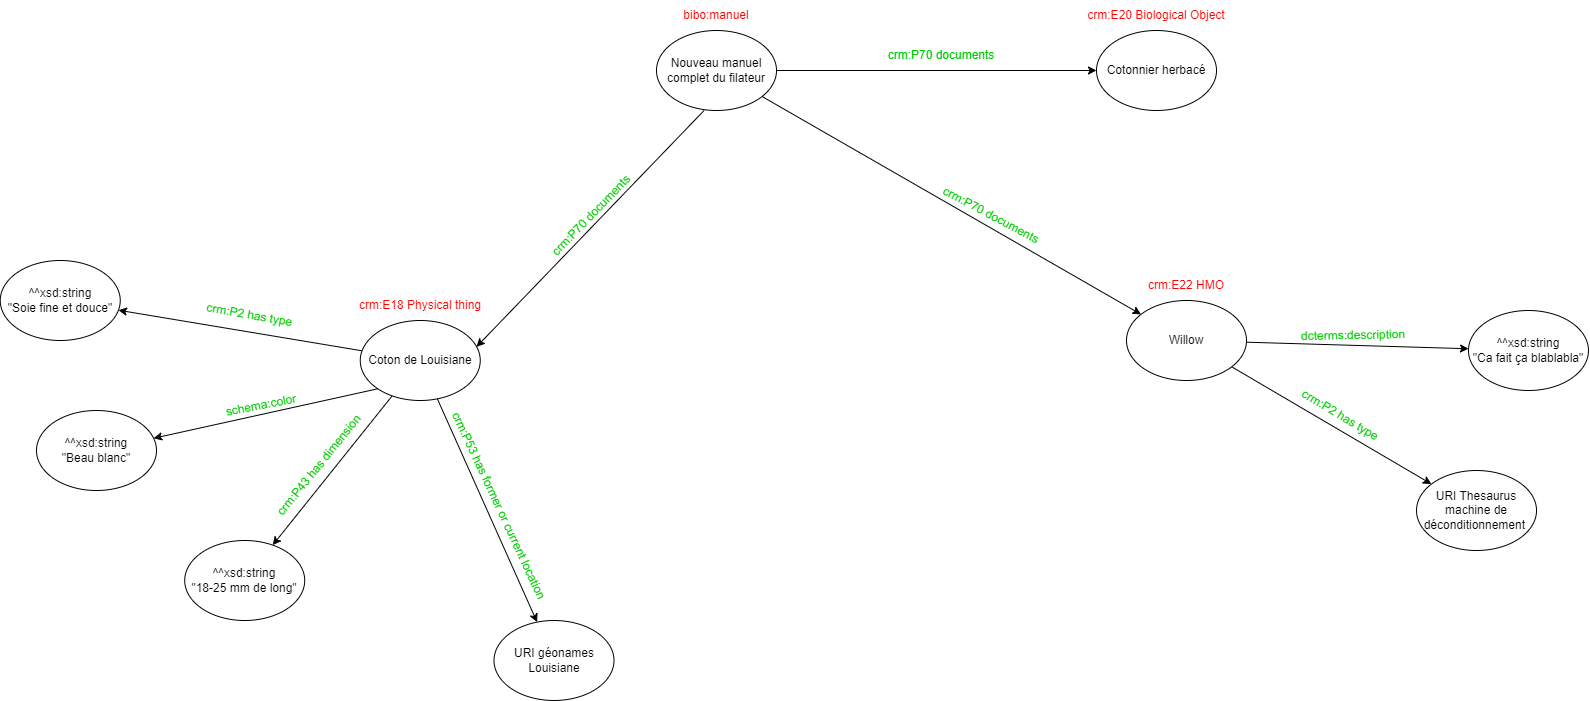
\includegraphics[width=1\textwidth]{assets/annexes/schema_manuel_roret.png}
    \caption{Schéma décrivant la production de fil de coton à l'aide du Manuel Roret}
    \label{fig:schemaRoretTTM}
\end{figure}

\addcontentsline{toc}{section}{Schéma décrivant les murs des bâtiments du Techn'hom}
\begin{figure} [H]
    \centering
    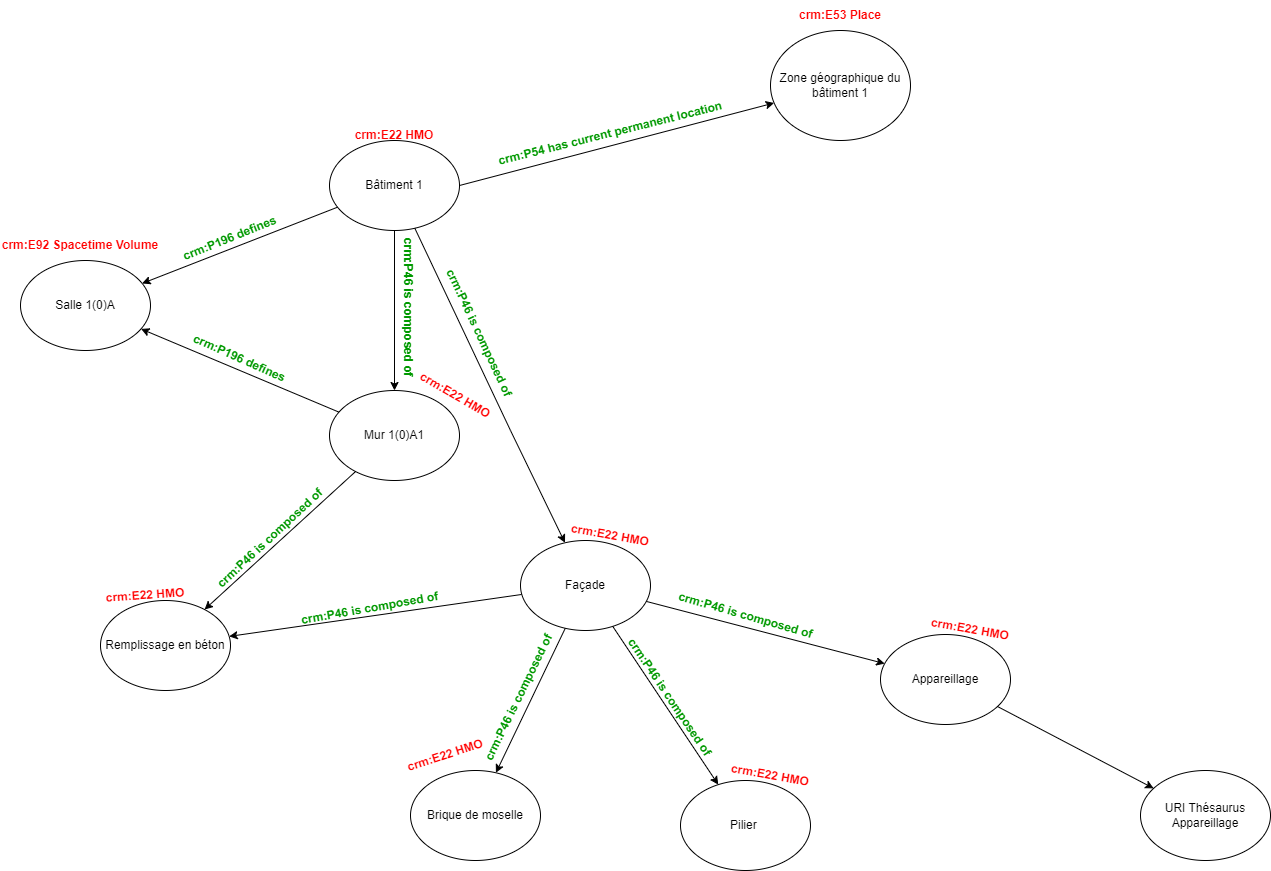
\includegraphics[width=1\textwidth]{assets/annexes/schema_desciption_mur.png}
    \caption{Schéma décrivant les murs des bâtiments du Techn'hom}
    \label{fig:schemaMursTTM}
\end{figure}

\section*{2. Graphe modélisant les relations entre ontologie}\label{annexe2}
\addcontentsline{toc}{section}{Graphe modélisant les relations entre ontologie}
\begin{figure} [H]
    \centering
    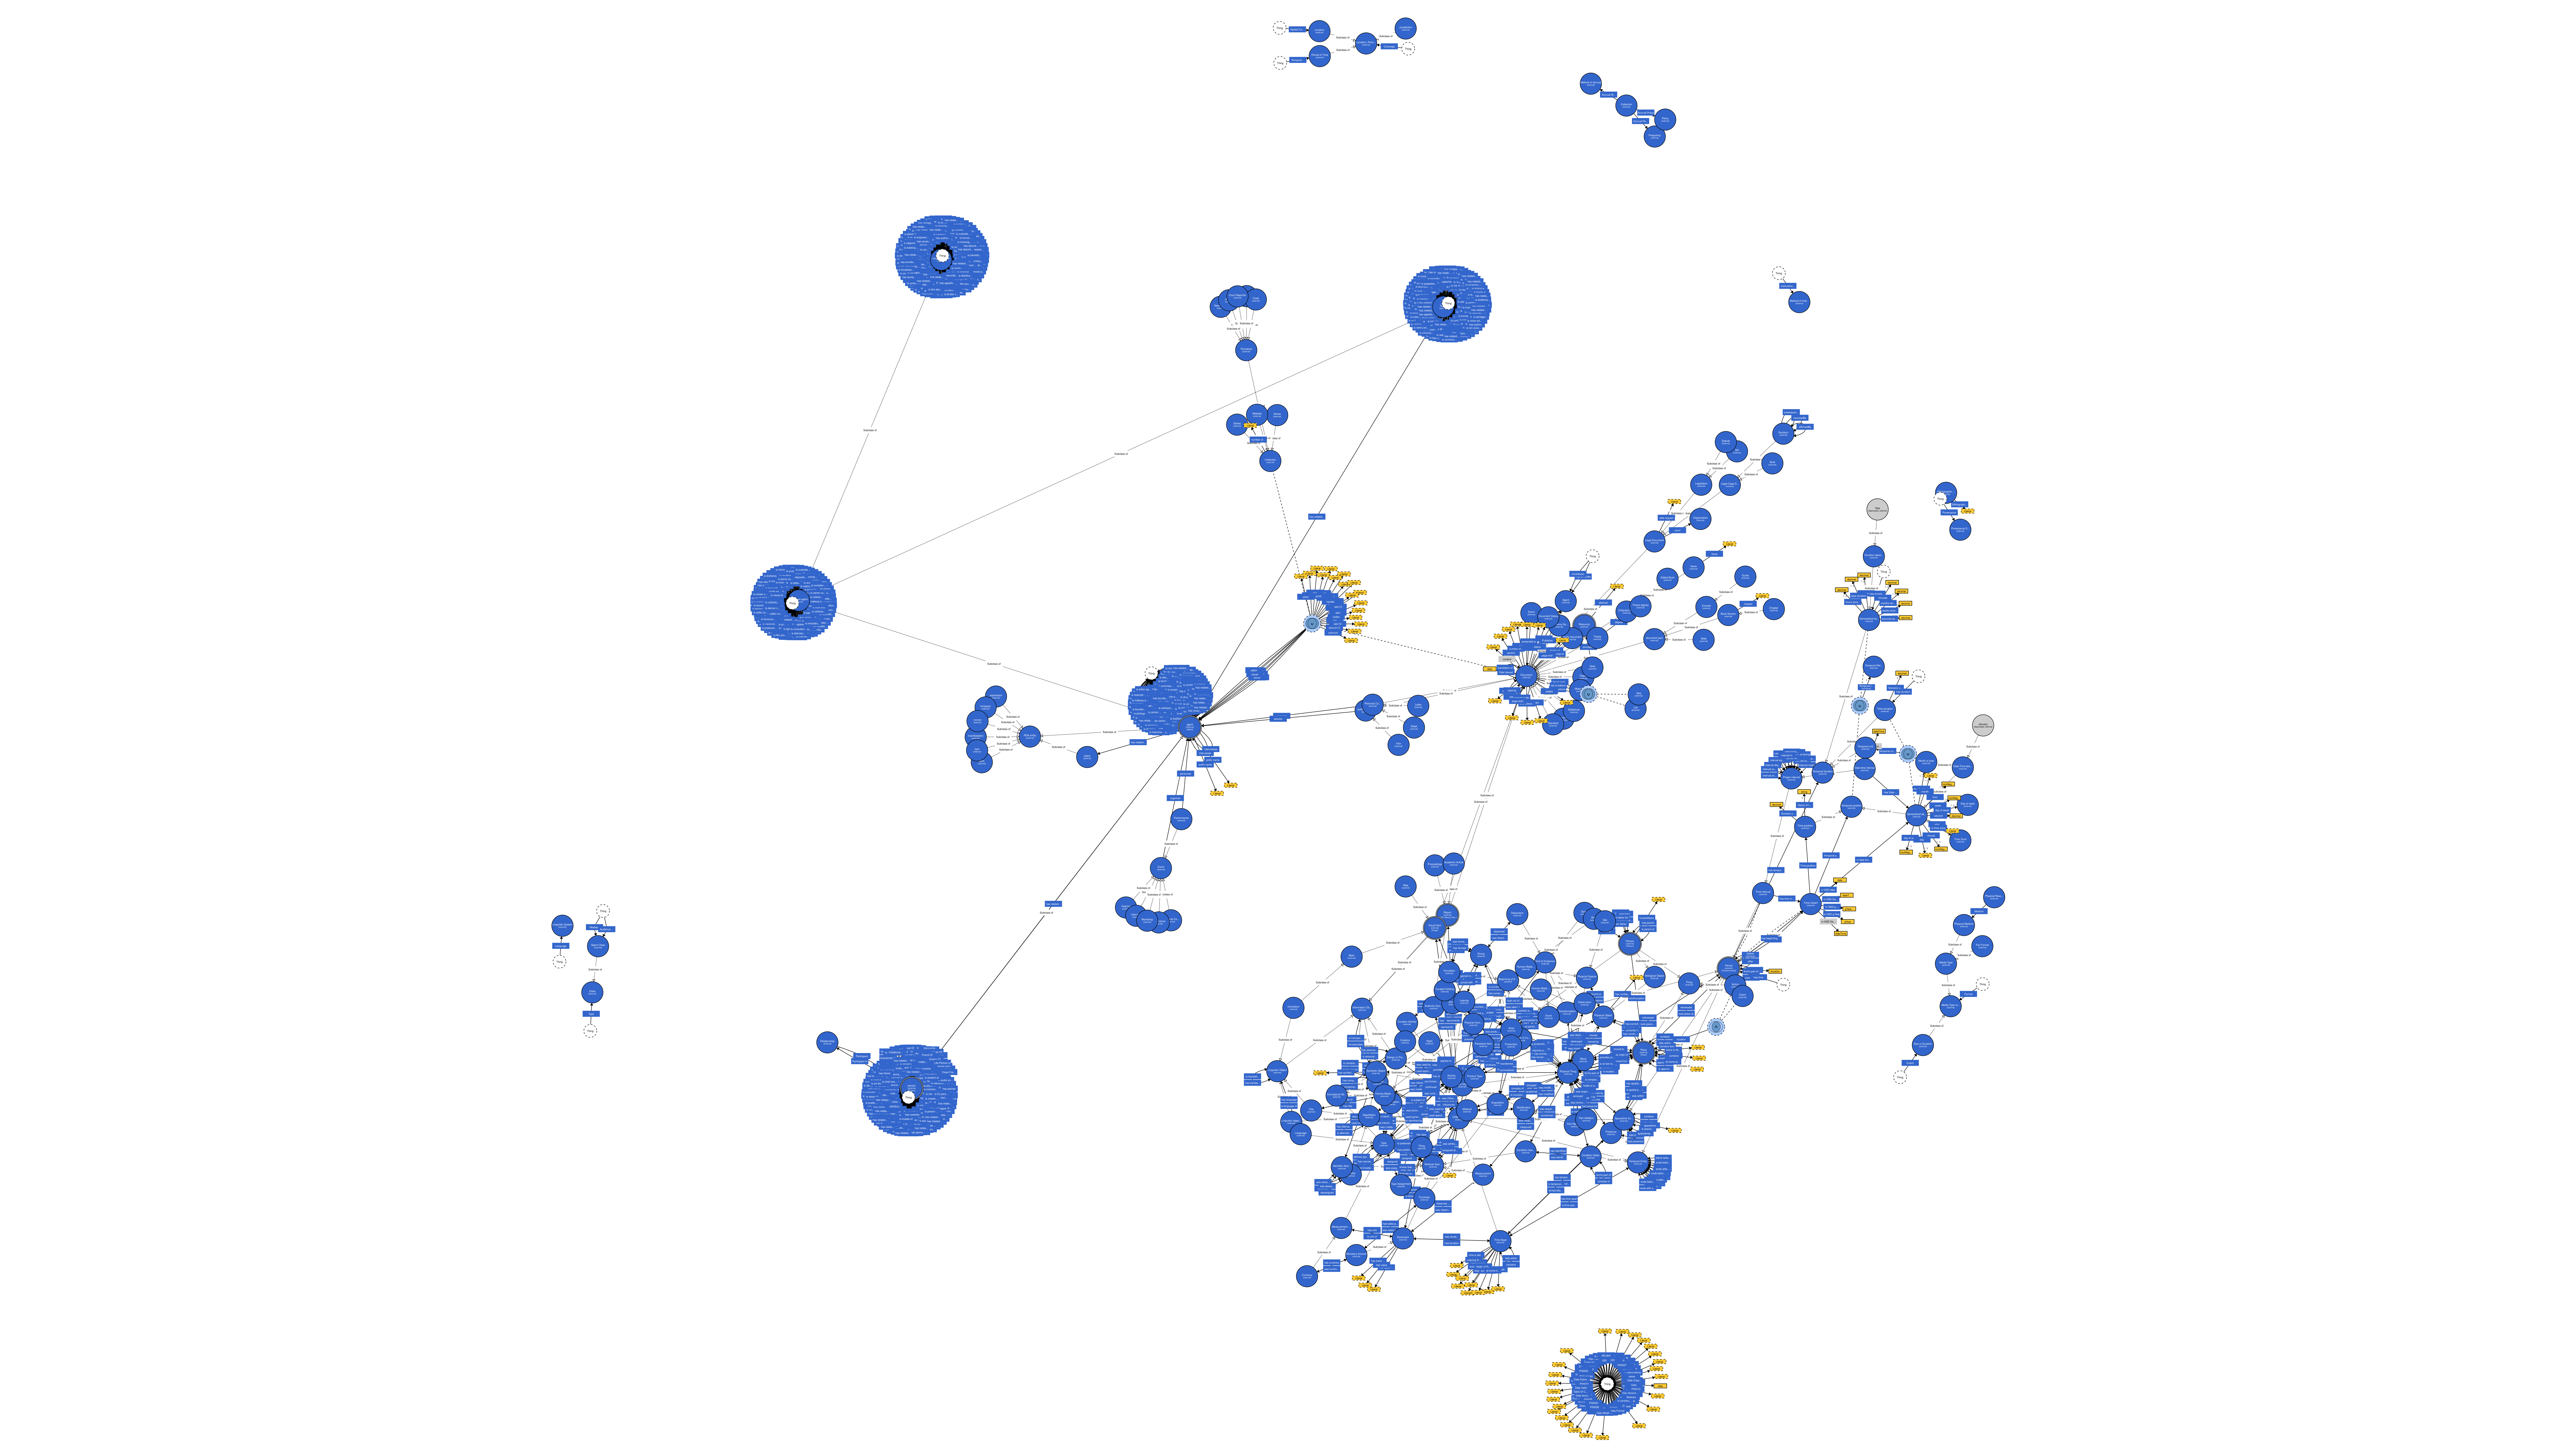
\includegraphics[width=1\textwidth]{assets/annexes/scheam_decla_ontologie.png}
    \caption{Graphe modélisant les relations théoriques entre ontologie}
    \label{fig:schemaGrapheOntologie}
\end{figure}

\section*{3. Application Omeka-S (vue site web)}\label{annexe3}
\addcontentsline{toc}{section}{Application Omeka-s (vue site web) - Page "Projet"}
\begin{figure} [H]
    \centering
    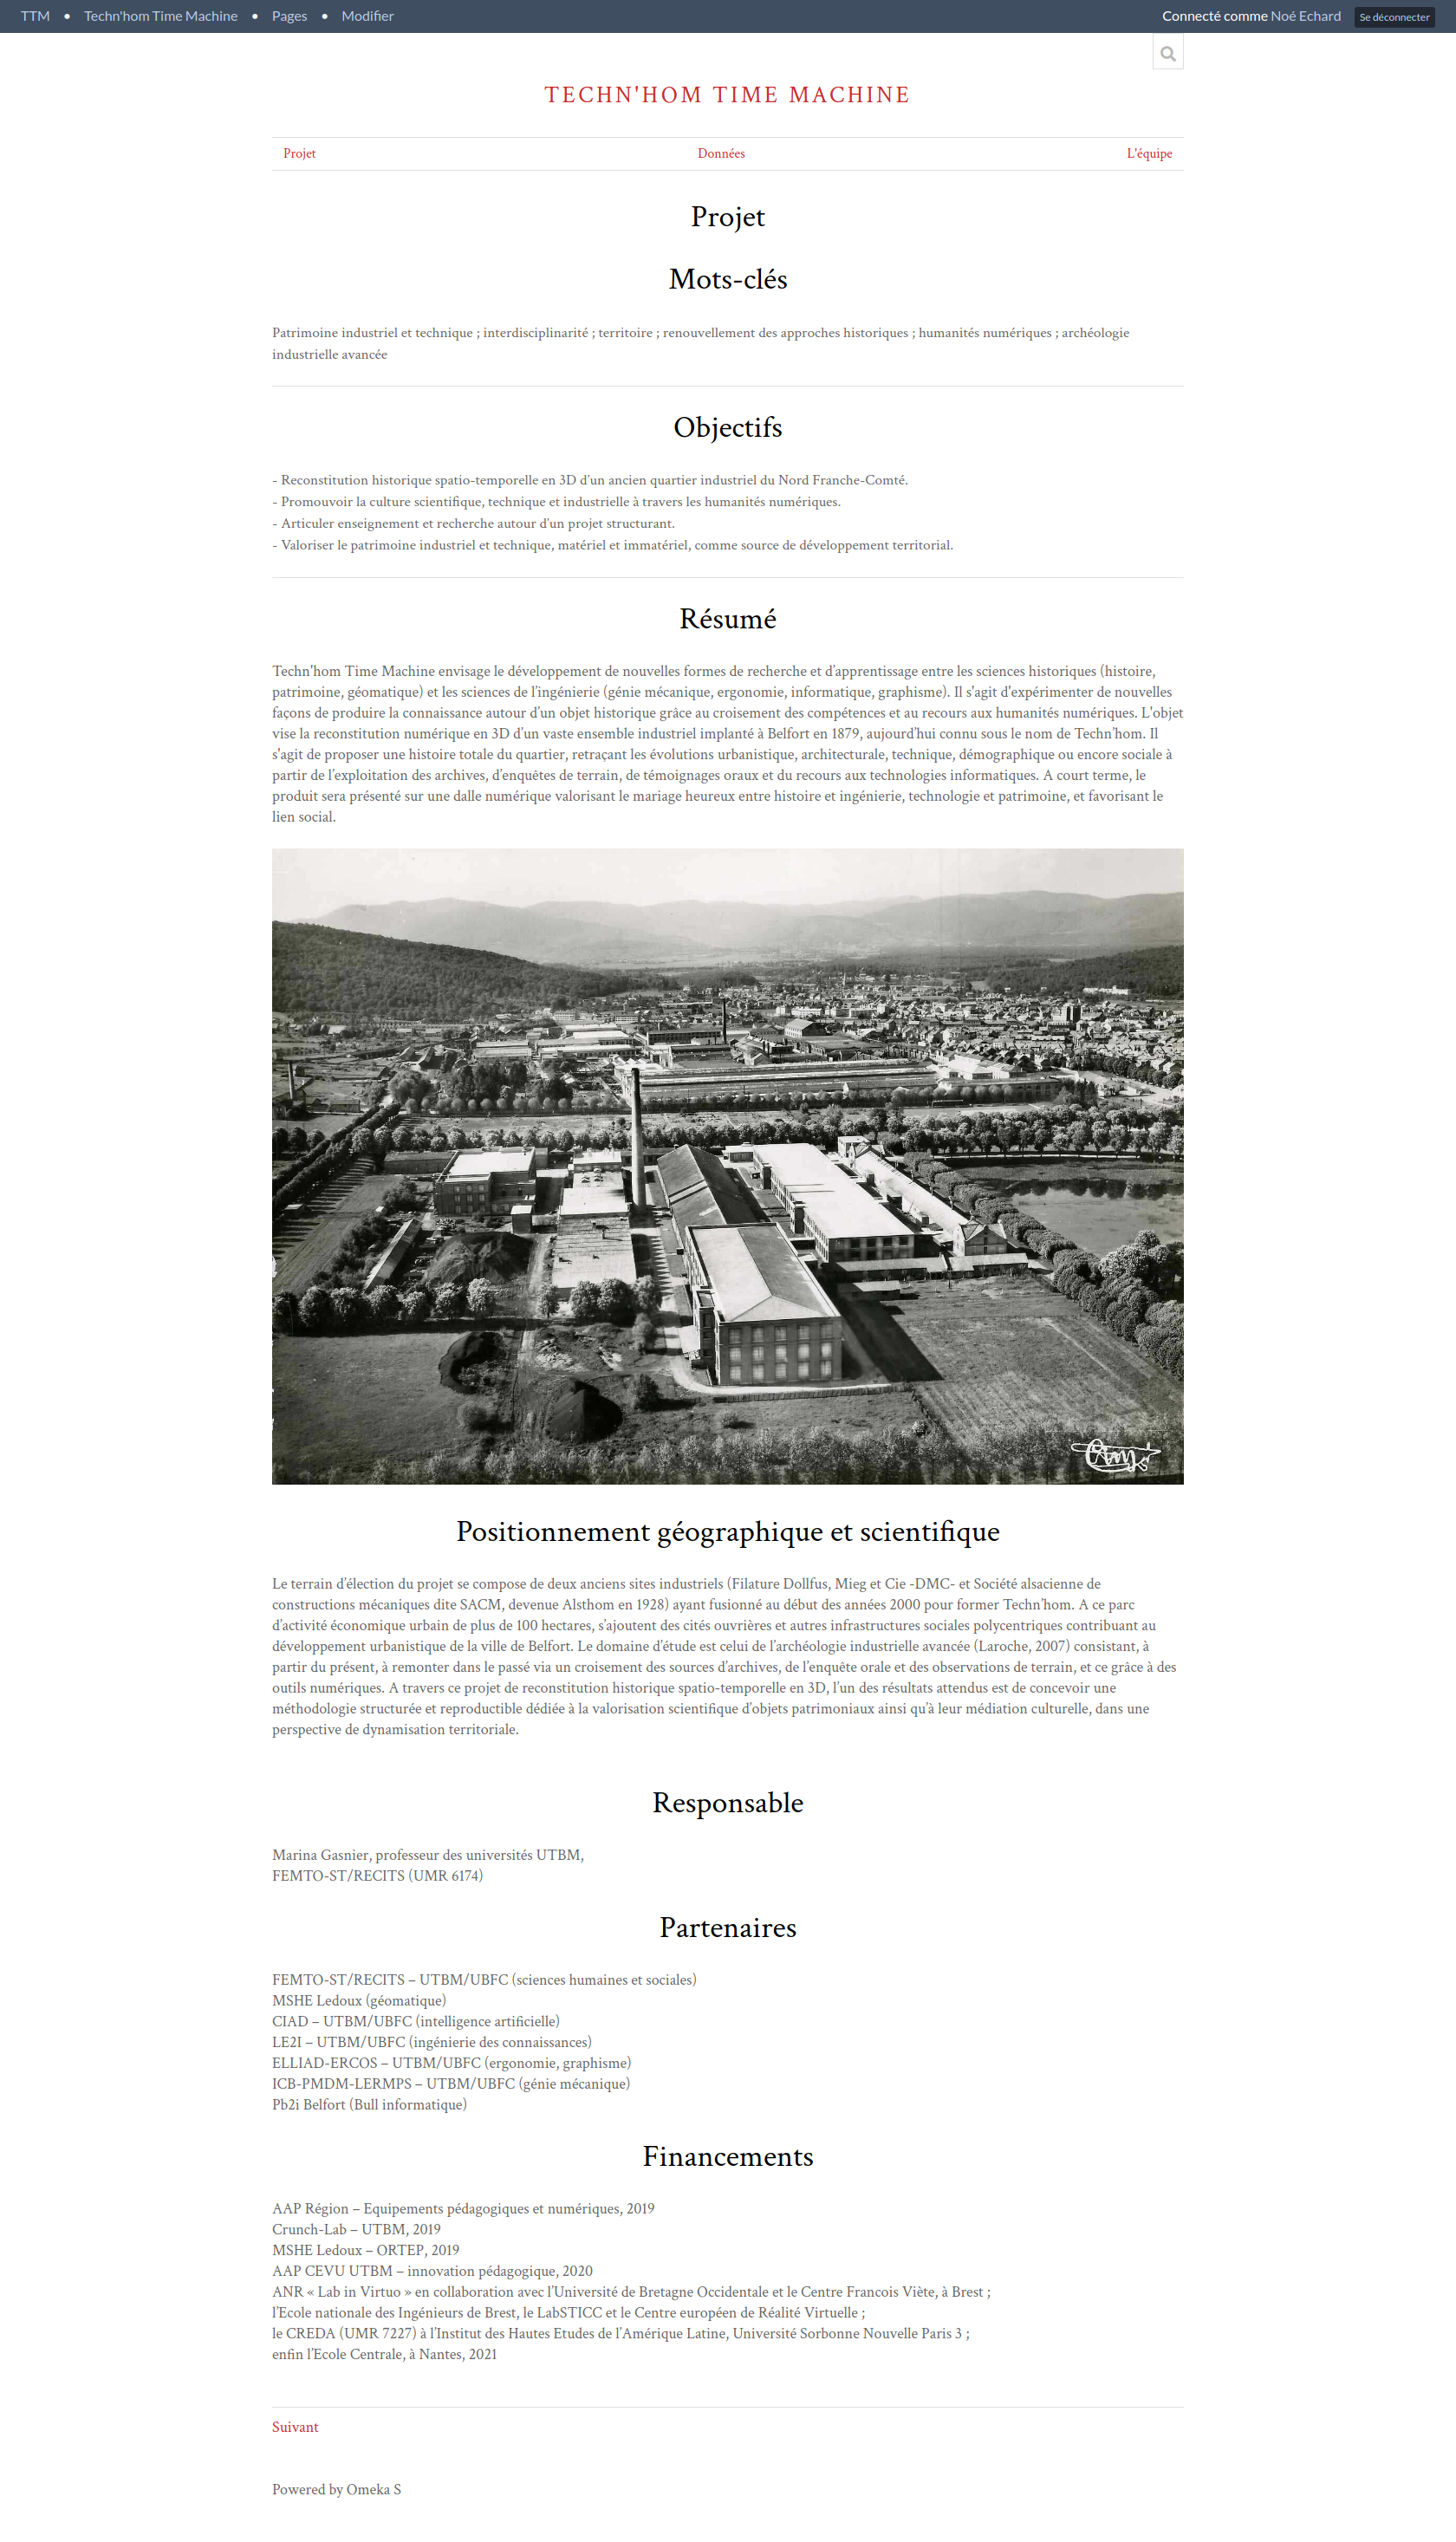
\includegraphics[width=0.8\textwidth]{assets/annexes/omeka_projet.png}
    \caption{Capture d'écran de la page "Projet" du site web du projet}
    \label{fig:pageProjetOmeka}
\end{figure}
\addcontentsline{toc}{section}{Application Omeka-s (vue site web) - Page "Equipe"}
\begin{figure} [H]
    \centering
    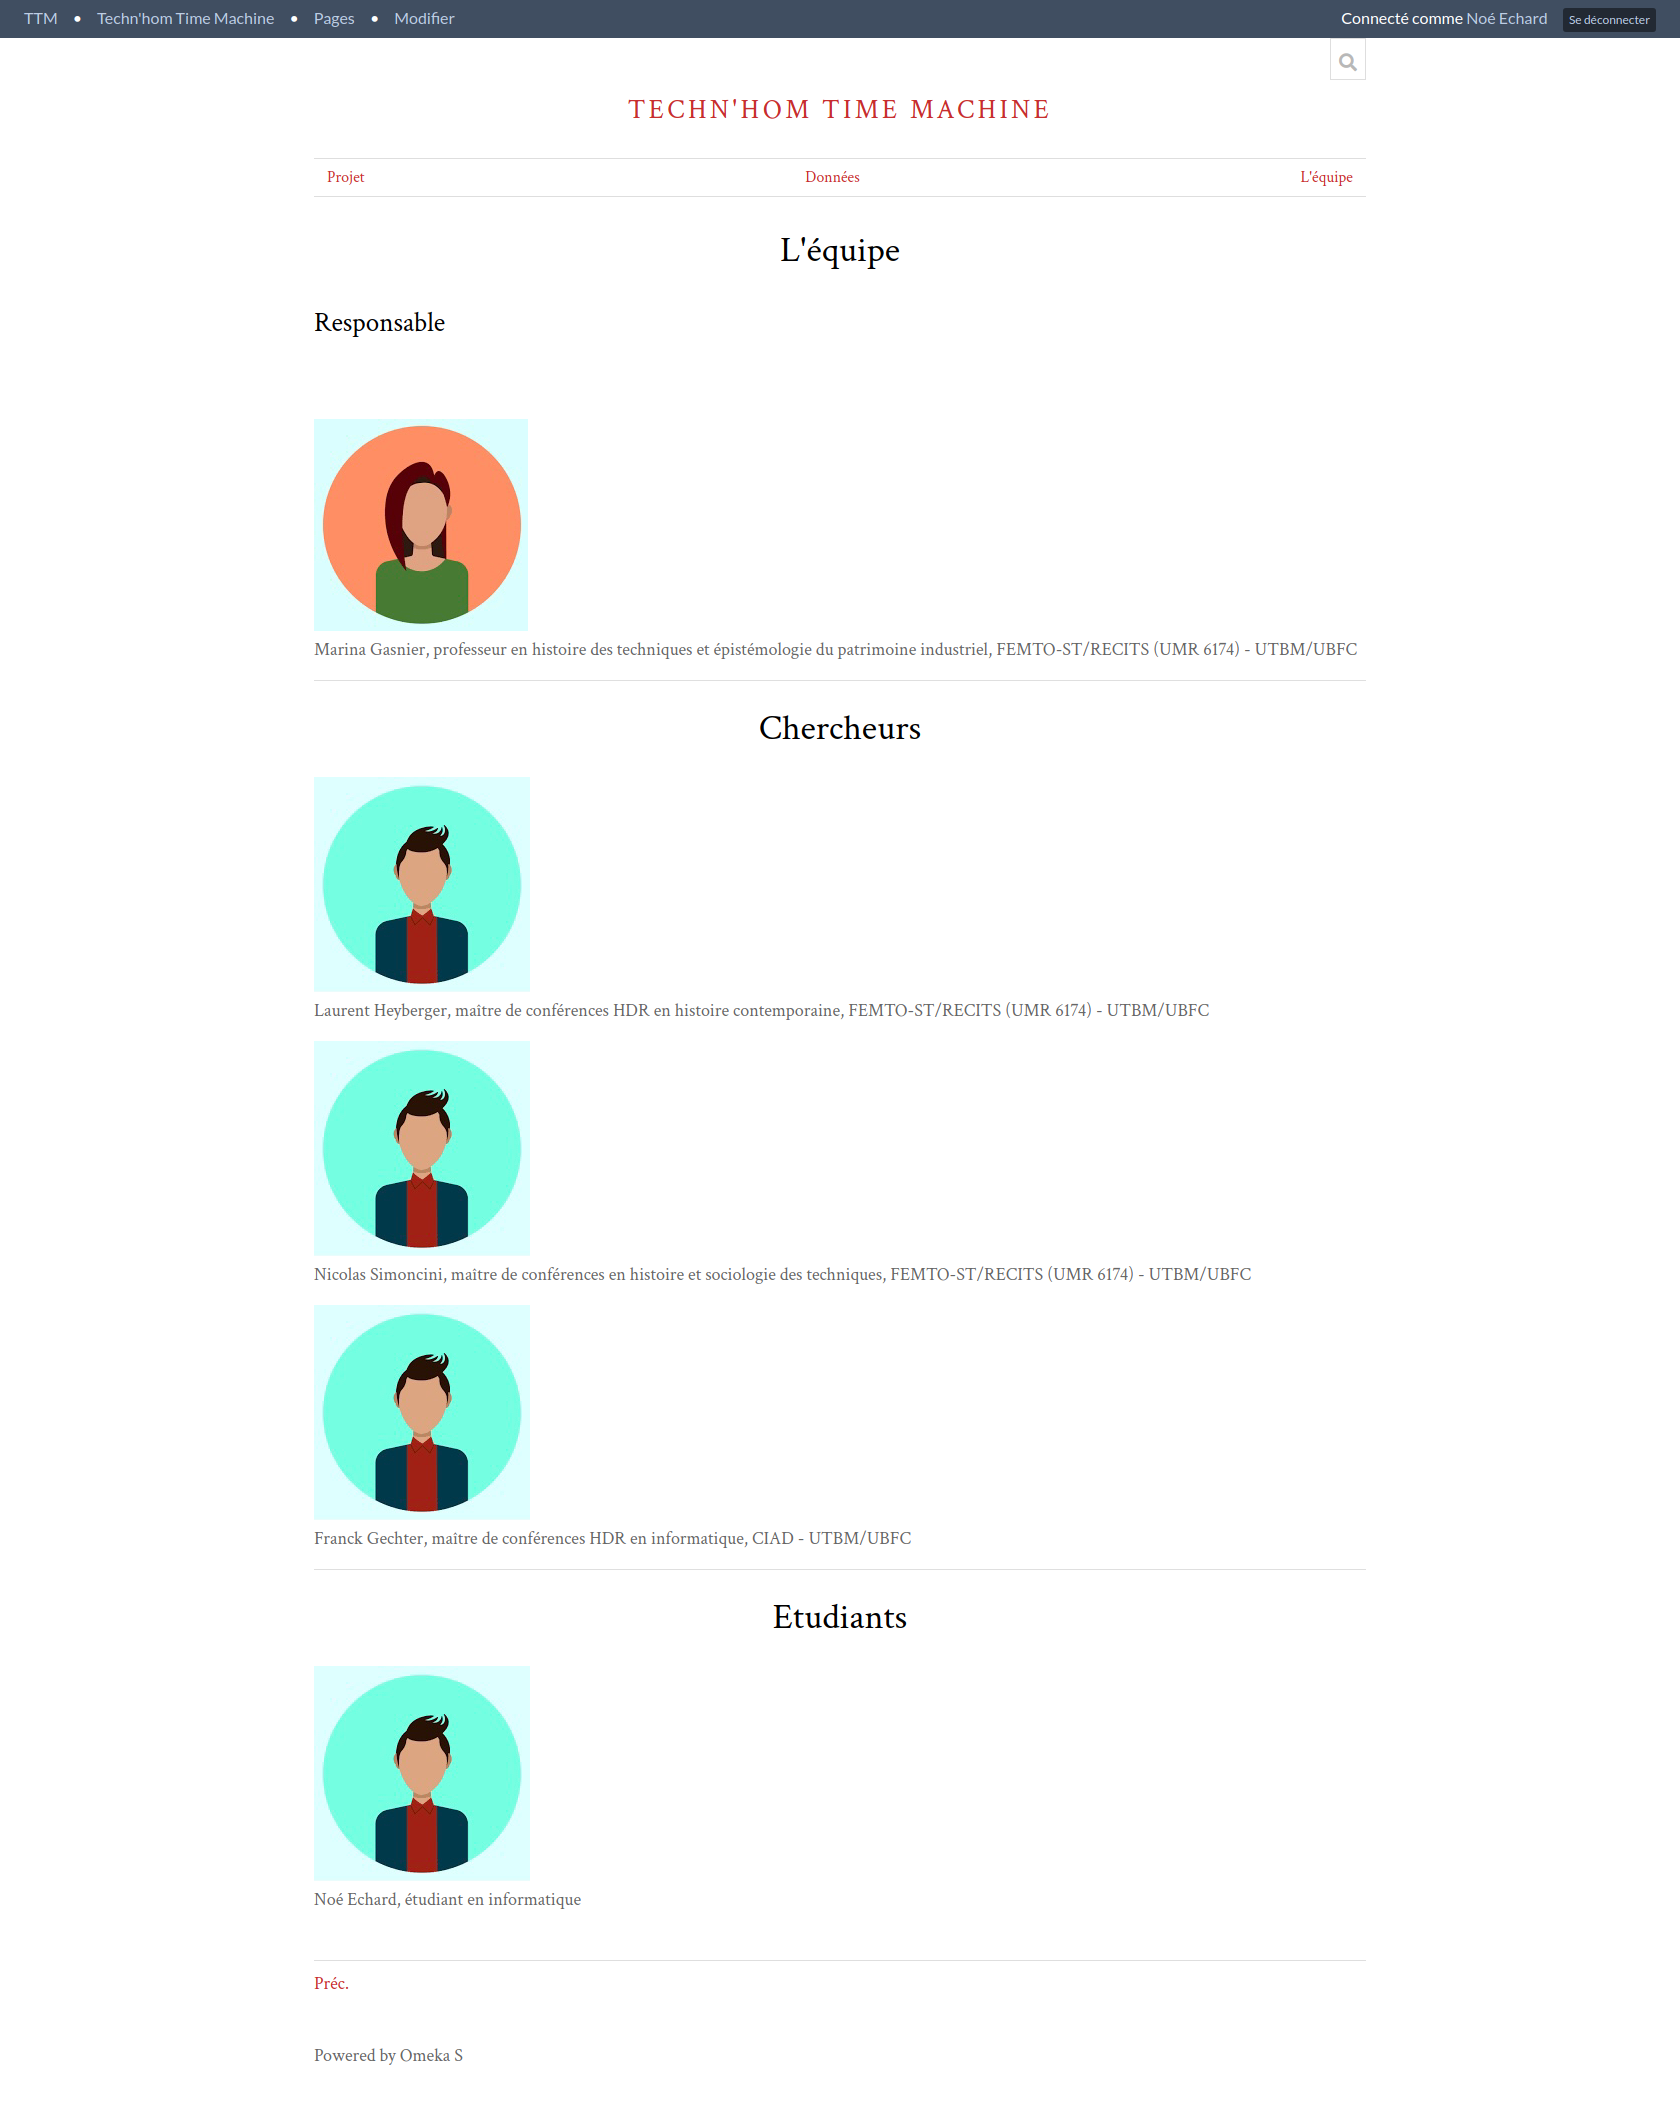
\includegraphics[width=1\textwidth]{assets/annexes/omeka_equipe.png}
    \caption{Capture d'écran de la page "Equipe" du site web du projet}
    \label{fig:pageEquipeOmeka}
\end{figure}
\addcontentsline{toc}{section}{Application Omeka-s (vue site web) - Page "Données"}
\begin{figure} [H]
    \centering
    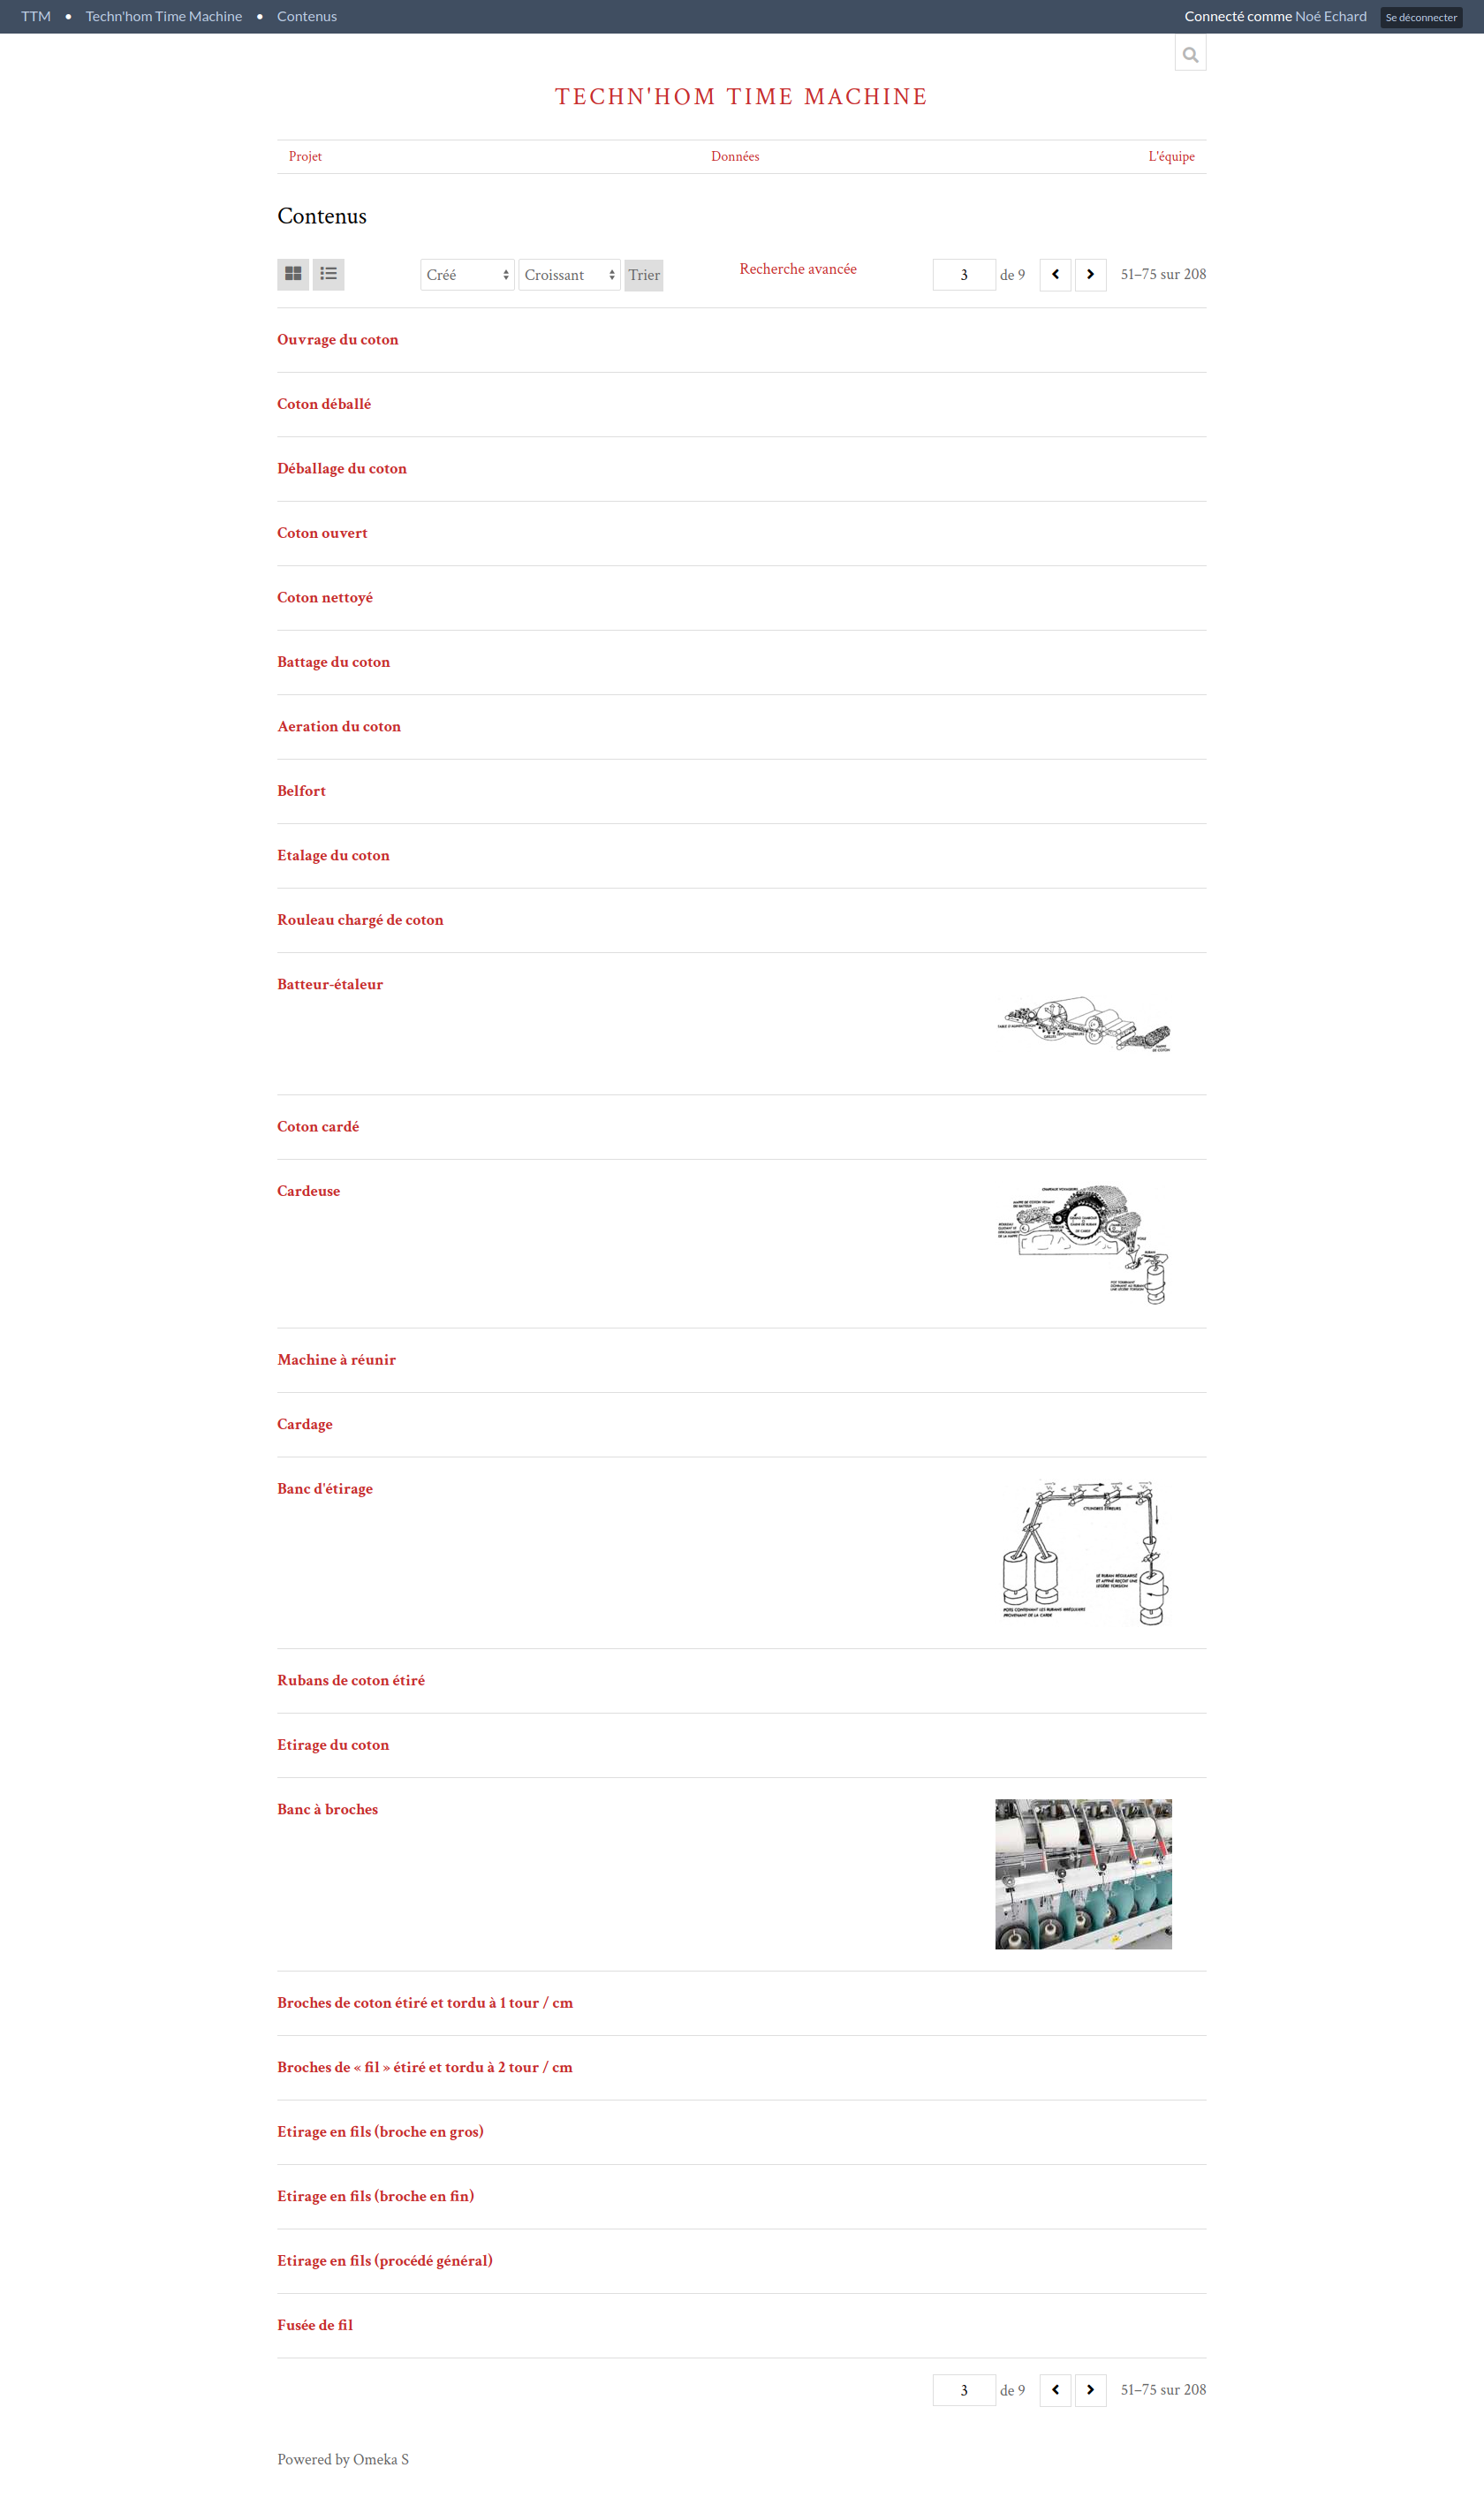
\includegraphics[width=0.8\textwidth]{assets/annexes/omeka_items.png}
    \caption{Capture d'écran de la page "Données" du site web du projet}
    \label{fig:pageDonnéesOmeka}
\end{figure}
\addcontentsline{toc}{section}{Application Omeka-s (vue site web) - Page de détail d'un item}
\begin{figure} [H]
    \centering
    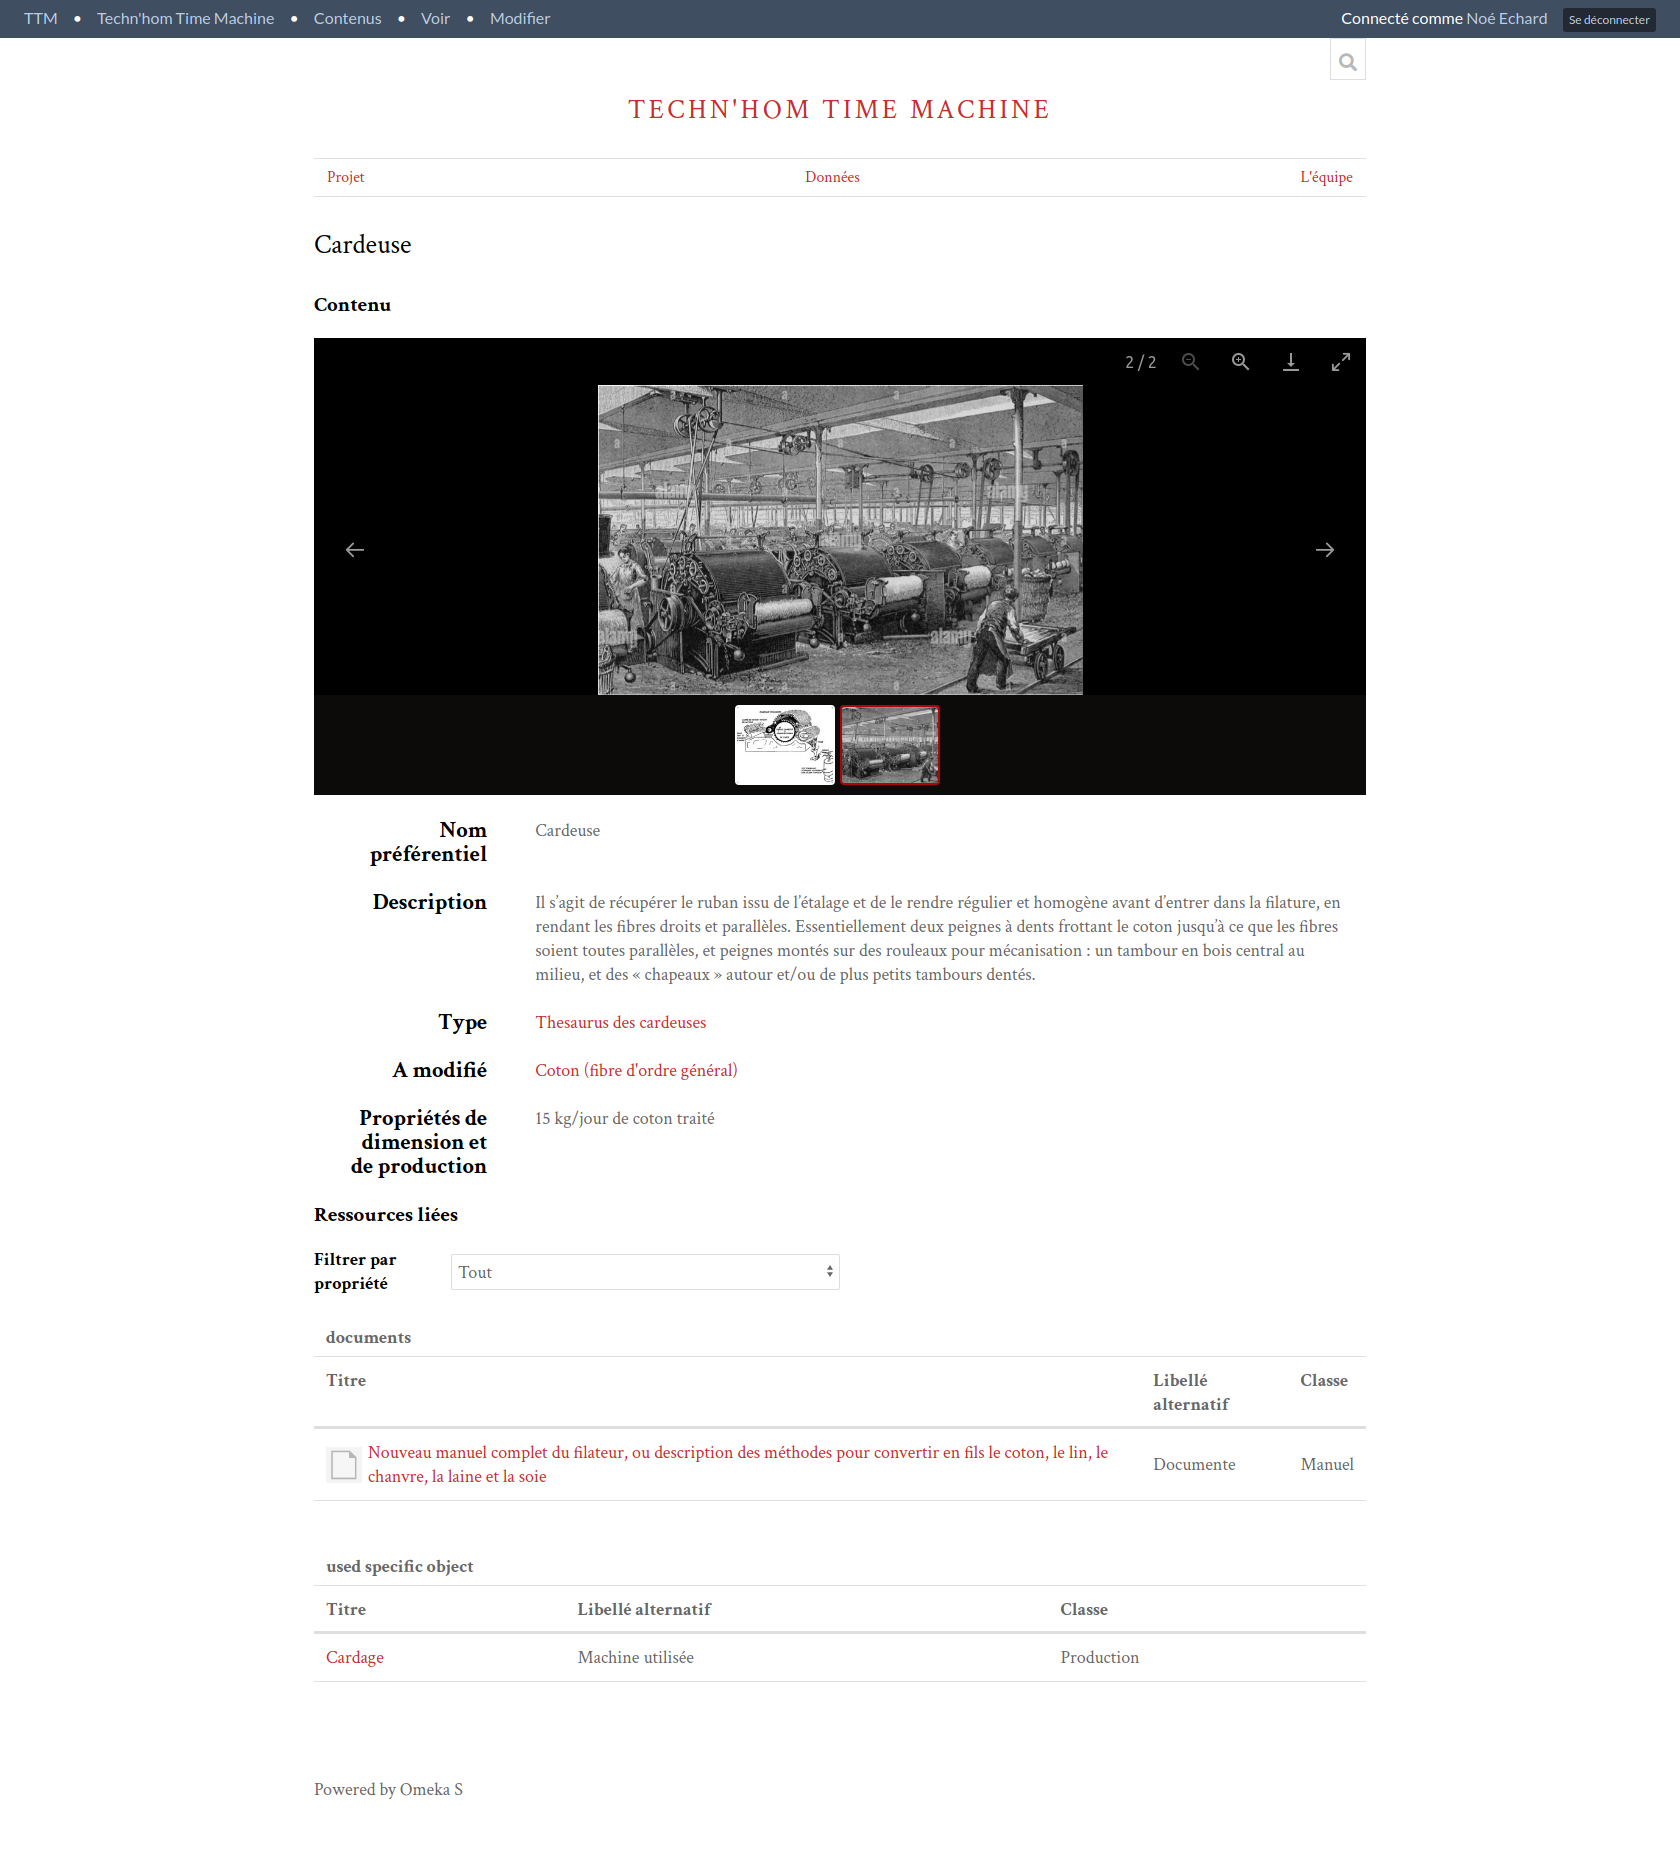
\includegraphics[width=0.8\textwidth]{assets/annexes/omeka_details.png}
    \caption{Capture d'écran de la page de détail d'un item du site web du projet}
    \label{fig:detailItemOmeka}
\end{figure}

\section*{4. Omeka-S}\label{annexe4}
\addcontentsline{toc}{section}{Omeka-S - Onglet "Contenus"}
\begin{figure} [H]
    \centering
    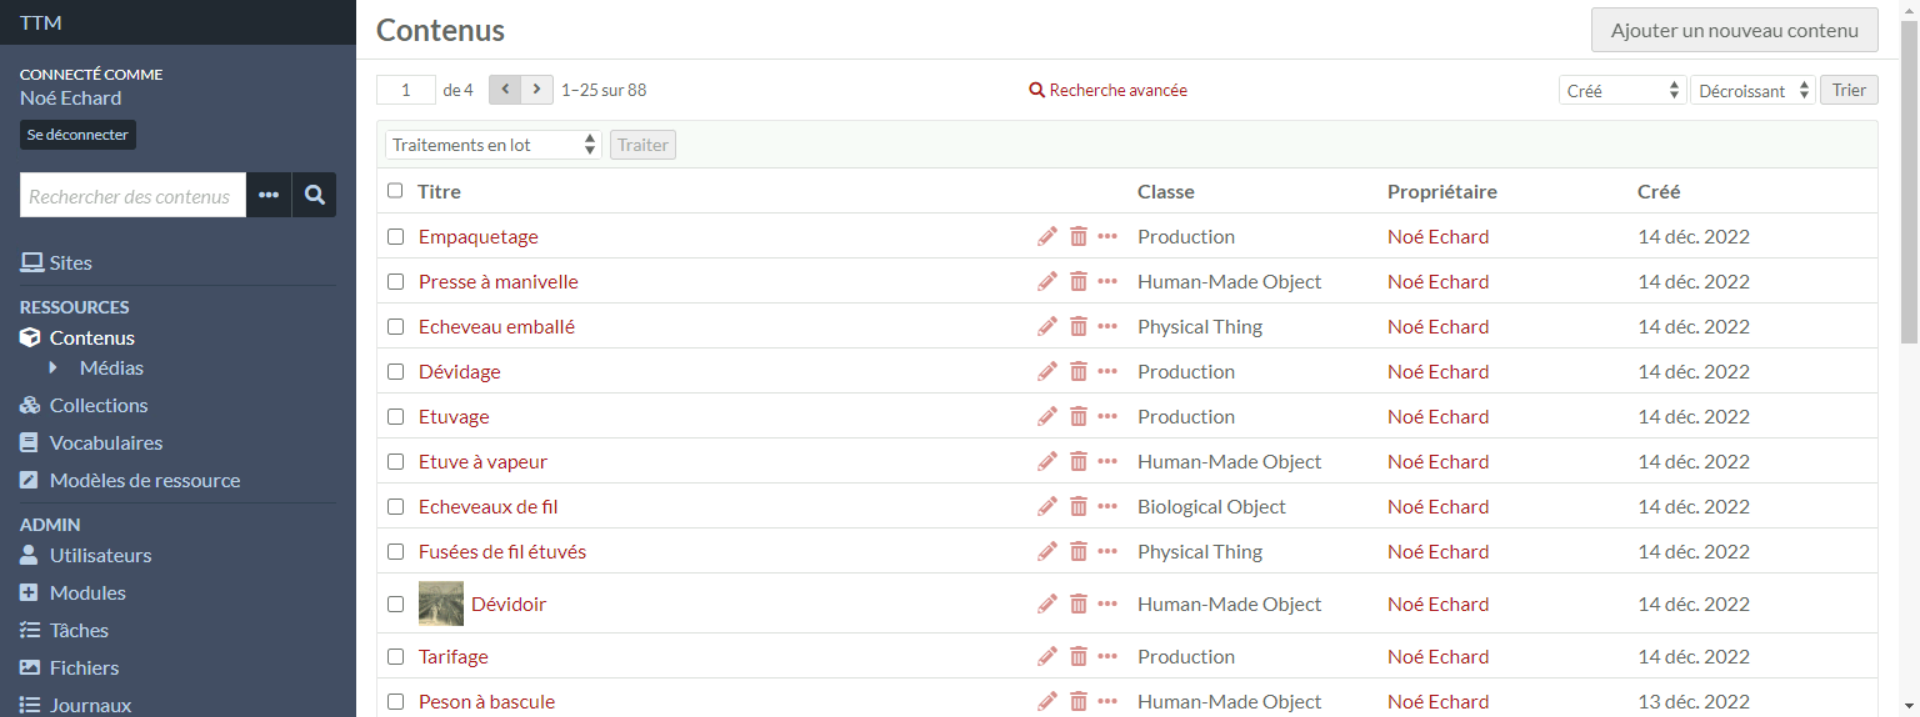
\includegraphics[width=1\textwidth]{assets/omeka/onglet_contenu_omeka.png}
    \caption{Capture d'écran de l'onglet contenus de Omeka-S}
    \label{fig:pageContenusOmeka}
\end{figure}

\addcontentsline{toc}{section}{Omeka-S - Onglet "Medias"}
\begin{figure} [H]
    \centering
    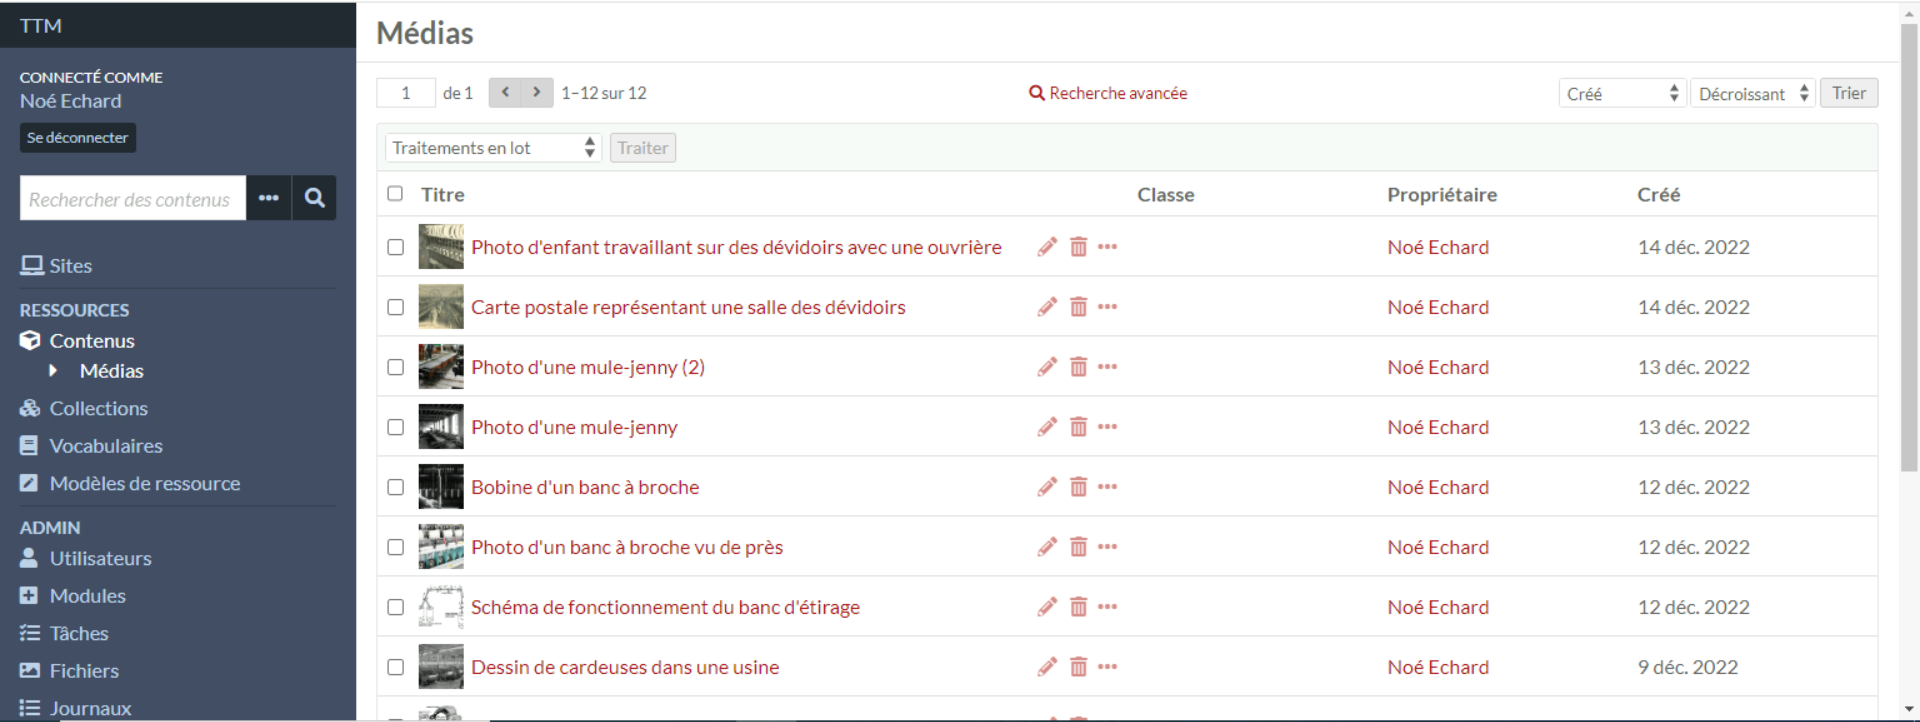
\includegraphics[width=1\textwidth]{assets/omeka/onglet_media_omeka.png}
    \caption{Capture d'écran de l'onglet medias de Omeka-S}
    \label{fig:pageMediasOmeka}
\end{figure}

\addcontentsline{toc}{section}{Omeka-S - Onglet "Modèles de ressources"}
\begin{figure} [H]
    \centering
    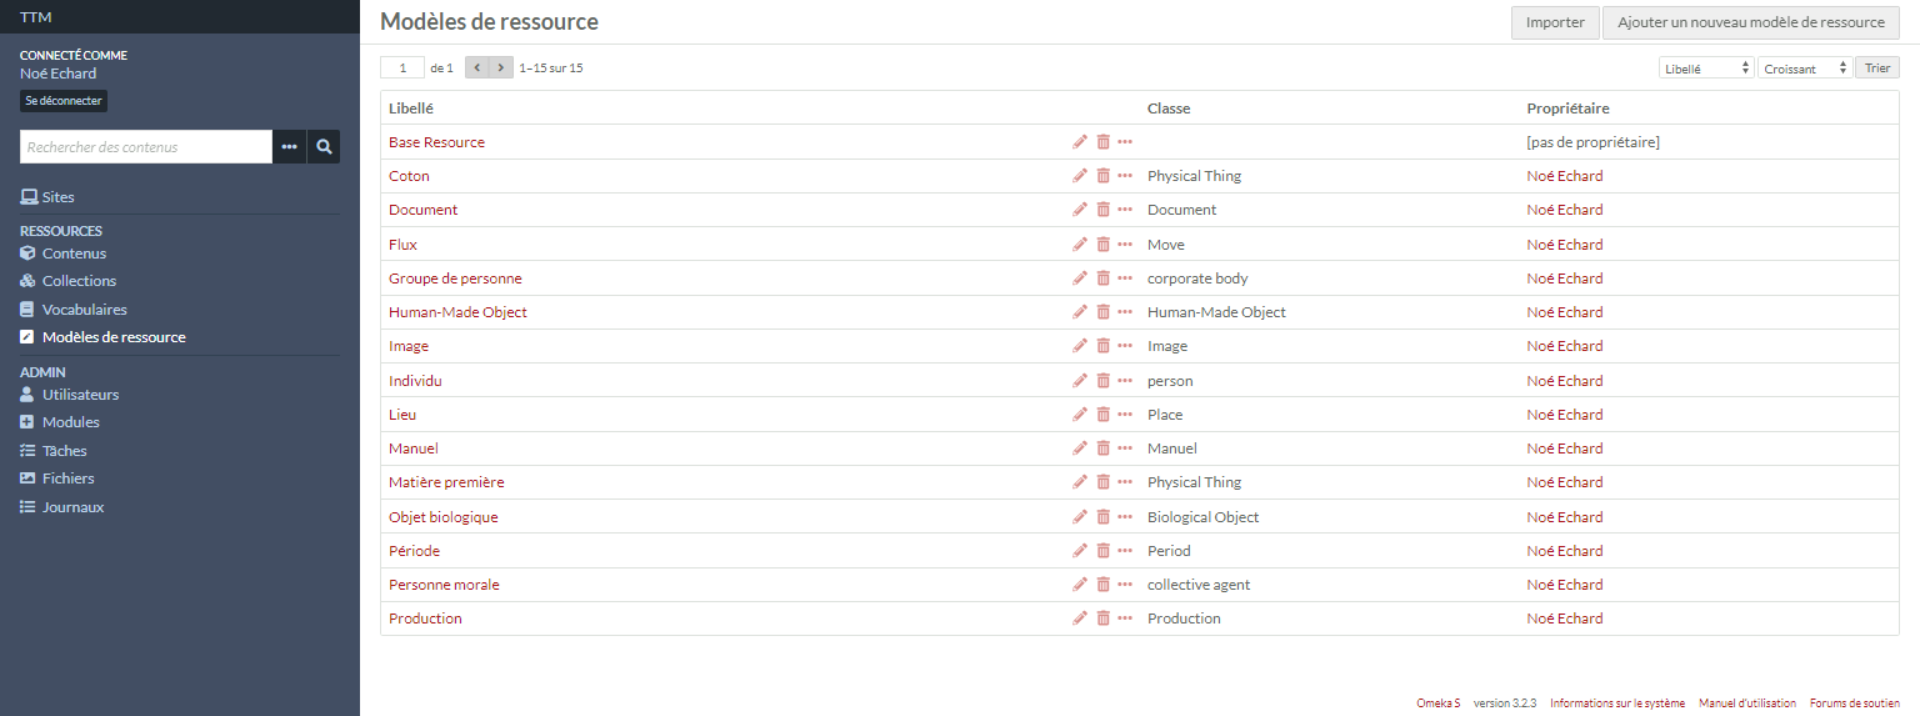
\includegraphics[width=1\textwidth]{assets/omeka/onglet_modele_ressource_omeka.png}
    \caption{Capture d'écran de l'onglet modèle de ressources de Omeka-S}
    \label{fig:pageModRessourceOmeka}
\end{figure}

\addcontentsline{toc}{section}{Omeka-S - Onglet "Users"}
\begin{figure} [H]
    \centering
    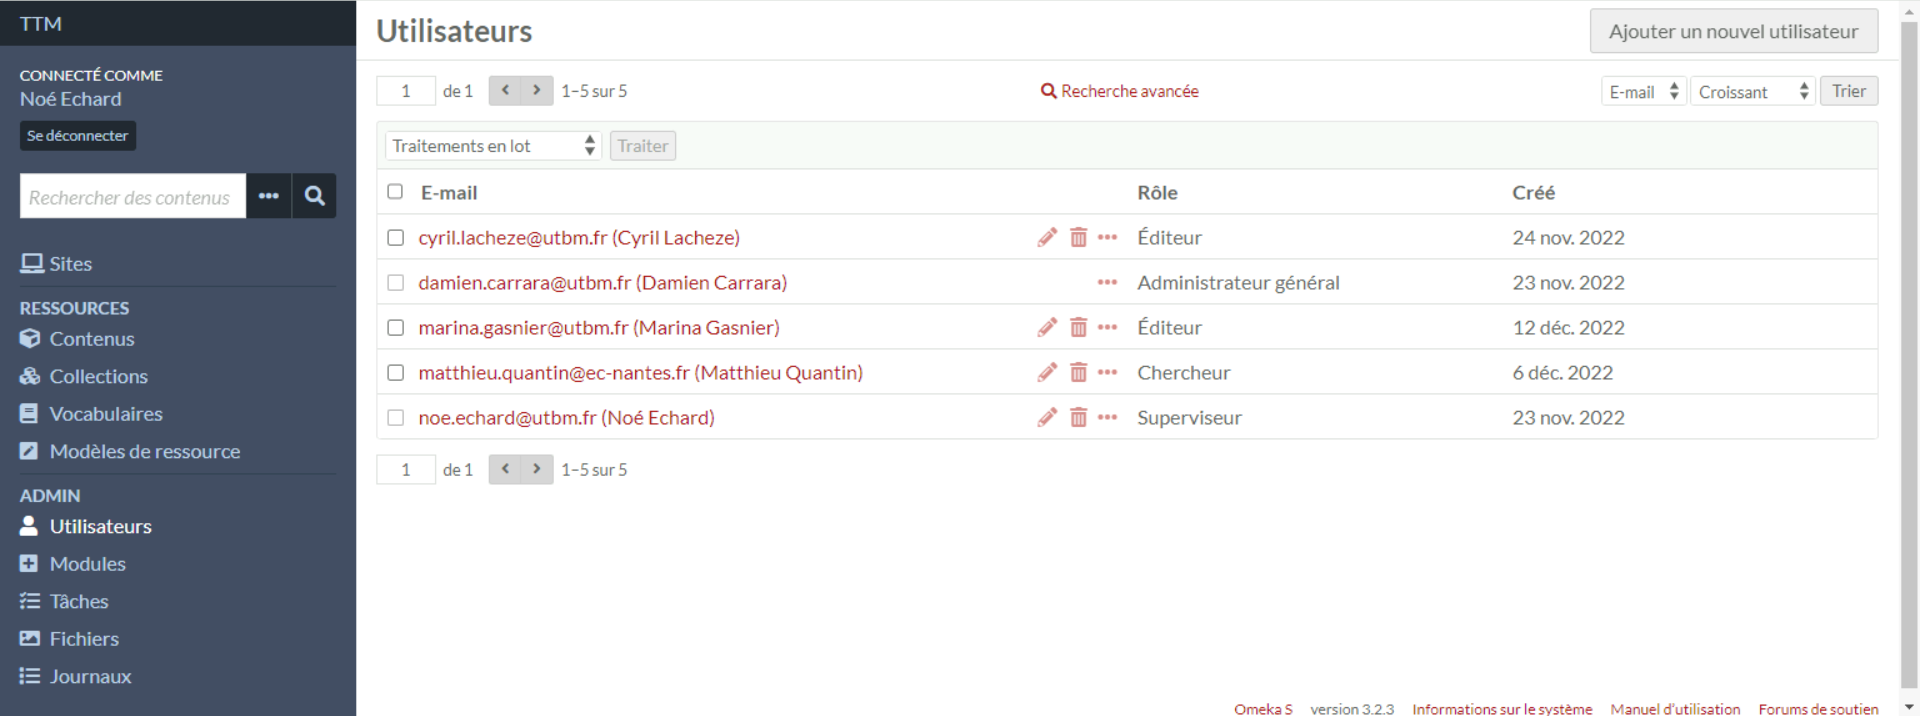
\includegraphics[width=1\textwidth]{assets/omeka/onglet_users_omeka.png}
    \caption{Capture d'écran de l'onglet users de Omeka-S}
    \label{fig:pageUsersOmeka}
\end{figure}

% AJOUTER DES SCREENS DU SITE WEB
% AJOUTER DES SCREENS DES FICHIERS DE L'ONTOLOGIE/SHACL
% AJOUTER DES SCREENS DU PROJET UNITY
        
	\makeutbmbackcover{}
\end{document}